% File name: trainingExperimentFinalAnalysis.R
% Author: Jacob Taylor
% Date: 20/09/2017
% Description: A script for analysing complete data from trainingExperiment in Weihai and Beijing during August 2016.
% This analysis incorporates performance data coded from video recordings of each experimental session.

\documentclass[english]{article}\usepackage[]{graphicx}\usepackage[]{color}
%% maxwidth is the original width if it is less than linewidth
%% otherwise use linewidth (to make sure the graphics do not exceed the margin)
\makeatletter
\def\maxwidth{ %
  \ifdim\Gin@nat@width>\linewidth
    \linewidth
  \else
    \Gin@nat@width
  \fi
}
\makeatother

\definecolor{fgcolor}{rgb}{0.345, 0.345, 0.345}
\newcommand{\hlnum}[1]{\textcolor[rgb]{0.686,0.059,0.569}{#1}}%
\newcommand{\hlstr}[1]{\textcolor[rgb]{0.192,0.494,0.8}{#1}}%
\newcommand{\hlcom}[1]{\textcolor[rgb]{0.678,0.584,0.686}{\textit{#1}}}%
\newcommand{\hlopt}[1]{\textcolor[rgb]{0,0,0}{#1}}%
\newcommand{\hlstd}[1]{\textcolor[rgb]{0.345,0.345,0.345}{#1}}%
\newcommand{\hlkwa}[1]{\textcolor[rgb]{0.161,0.373,0.58}{\textbf{#1}}}%
\newcommand{\hlkwb}[1]{\textcolor[rgb]{0.69,0.353,0.396}{#1}}%
\newcommand{\hlkwc}[1]{\textcolor[rgb]{0.333,0.667,0.333}{#1}}%
\newcommand{\hlkwd}[1]{\textcolor[rgb]{0.737,0.353,0.396}{\textbf{#1}}}%
\let\hlipl\hlkwb

\usepackage{framed}
\makeatletter
\newenvironment{kframe}{%
 \def\at@end@of@kframe{}%
 \ifinner\ifhmode%
  \def\at@end@of@kframe{\end{minipage}}%
  \begin{minipage}{\columnwidth}%
 \fi\fi%
 \def\FrameCommand##1{\hskip\@totalleftmargin \hskip-\fboxsep
 \colorbox{shadecolor}{##1}\hskip-\fboxsep
     % There is no \\@totalrightmargin, so:
     \hskip-\linewidth \hskip-\@totalleftmargin \hskip\columnwidth}%
 \MakeFramed {\advance\hsize-\width
   \@totalleftmargin\z@ \linewidth\hsize
   \@setminipage}}%
 {\par\unskip\endMakeFramed%
 \at@end@of@kframe}
\makeatother

\definecolor{shadecolor}{rgb}{.97, .97, .97}
\definecolor{messagecolor}{rgb}{0, 0, 0}
\definecolor{warningcolor}{rgb}{1, 0, 1}
\definecolor{errorcolor}{rgb}{1, 0, 0}
\newenvironment{knitrout}{}{} % an empty environment to be redefined in TeX

\usepackage{alltt}
\usepackage[utf8]{inputenc}
\usepackage[margin=1.8cm,a4paper]{geometry}
\usepackage[english]{babel} % hyphenation
\usepackage{csquotes}
\usepackage{amsmath,amssymb,amsthm} % for mathematical
\usepackage{graphicx} % to include graphics
\newcommand{\myparagraph}[1]{\paragraph{#1}\mbox{}\\}


%Bib Setup:

\usepackage[style=apa, sorting=nyt, backend=biber, maxcitenames=2, useprefix=true, doi=false, isbn=false, natbib=true, language=american]{biblatex}
\DeclareLanguageMapping{american}{american-apa}
\newcommand*{\bibtitle}{Works Cited}
\addbibresource{references.bib}

% Main data manipulation tasks: 1) data reduction (group and team measures)
%                               2) group differences
%                               3) manipulation checks

% Main objectives: 1) test study predictions:

%                     1.a relationship between perceived joint action success and team click
%                             1.a.i relationship between session performance variables and perceptions of joint action success / team click?
%                     1.b relationship between expectation violation and team click
%                             1.b.i relationship between session performance variables and expectation violation / team click?
%                     1.c interaction between perceptions of jointActionSuccess and teamClick
%
%                     2.a relationship between team click and social bonding
%                             (2.a.i relationship between performance and social bonding?)
%
%                     3.a relationship between jointActionSuccess and socialBonding?
%                         3.a.i relationship between performance and socialBonding
%                     3.b relationship between expectation violation and socialBonding
%
%                     4.a mediation analysis: teamClick mediates relationship between jointActionSuccess and socialBonding
%                         4.a.i jointActionSuccess mediates relationship between performance and teamClick?
%                     4.b mediation analysis: teamClick mediates relationship between Expectations and socialBonding
%
%                     2.1.a - 2.4.b ---> re run this looking at pre-post changes in group measures and team measures...
%                     Additional analyses:
%                               1. teamClick mediates relationship between jointAction and generalised socialBonding to team / family?
%                               2.

% setting global settings and loading useful libraries
\IfFileExists{upquote.sty}{\usepackage{upquote}}{}
\begin{document}

\begin{knitrout}
\definecolor{shadecolor}{rgb}{0.969, 0.969, 0.969}\color{fgcolor}\begin{kframe}


{\ttfamily\noindent\color{warningcolor}{\#\# Warning: package 'tableone' was built under R version 3.3.2}}

{\ttfamily\noindent\color{warningcolor}{\#\# Warning: package 'apa' was built under R version 3.3.2}}

{\ttfamily\noindent\color{warningcolor}{\#\# Warning: package 'ggplot2' was built under R version 3.3.2}}\end{kframe}
\end{knitrout}




\title{Field Experiment}
\date{}
\author{Jacob Taylor & Emma Cohen \\ Institute of Cognitive \and Evolutionary Anthropology, University of Oxford}



\section{Abstract}
This study further tested the relationship, hypothesised in this dissertation, between joint action, team click, and social bonding in a controlled experimental environment.  An experiment was designed to test the prediction, partly confirmed in an in situ survey study, that athletes who experienced higher quality joint action would also experience higher levels of team click and social bonding.  58 Professional Chinese rugby players (Men = 31) participated in a between-subjects design in which athletes' expectations for joint action training drill \citep[``Invasion drill''][]{Passos2011}) were manipulated in one of two conditions.  Athletes in the ``low difficulty'' condition were primed with information to suggest that the training drill would require minimal rugby-sepcific individual and joint-action competence (i.e., 2/10 difficulty rating).  By contrast, in the ``high difficulty'' condition, athletes were primed to expect the training drill to be relatively difficult (8/10 difficulty rating). Pre- and post-experiment surveys were conducted, measuring athletes' perceptions of main variables of interest (individual and group performance, team click, and social bonding (both to the training group and the team more generally)), as well as athlete personality type and states of athlete states of arousal, fatigue, and injury.  Video footage of each experimental session was also recorded to derive an objective measure of interpersonal coordination not reliant on self-report.

It was predicted that athletes in the high-uncertainty condition would experience higher levels of team click and social bonding for two reasons: 1) athletes with expectations of higher difficulty would pay greater attention to coordinating action with others, and 2) athletes expecting higher difficulty in the experiment would experience higher positive violation of expectations around group performance.  Athletes in the ``low difficulty'' condition would on average experience less strongly the phenomenon of ``team click'' and flow-on feelings of social bonding, because they were not primed to attend less closely to joint-action with co-actors, and they would not experience the same level of positive violations of expectations around group performance.   Video footage was analysed for evidence of dynamic coupling between co-actors as well as defenders \citep{Schmidt2011,Richardson2012,Passos2012}, and these data were compared to psychological measures in order to explore psychological correlates of effective  interpersonal movement coordination in joint action.


\section{Introduction}
When athletes coordinate their behaviours they do so by making predictions about the state of the world.  In the case of joint action, in which there are many moving parts, predictions rely on the behaviours of
of others for their accuracy. Annecdote and observation in team sport and other joint activities involving complex realtime coordination of behaviours around technically demanding tasks, suggests that the phenomenology associated with co-actors' predictions clicking into place is an extremely powerful social bonding agent.

The previous chapter presented empirical evidence of a relationship between perceptions of joint action success and social bonding, fully mediated by the phenomenon of ``team click.'' A relationship between violation of expectations surrounding team performance and feelings of team click was also observed, but a model of the relationship between team performance expectation vioaltion and social bonding did not reliably fit the data.  The results of this naturalistic \textit{in situ} study are noteworthy as they provide evidence for the prediction that perceptions of joint action influence psychological processes of affiliation and connection with teammates, possibly via the mediating phenomenon of ``team click.''  Controlled experimental research is needed in order to more directly access causal mechanisms that underpin the relationship between joint action and social bonding.  If perceived joint action success and positive violation of expectation around team performance are the two candidate predictors of team click and social bonding, how is it possible to experimentally manipulate conditions conducive to maximising these two factors in joint action? In addition, how is it possible to isolate joint action from other potential sources of information regarding the team and its performance such as explicit feedback from coaches and other players surrounding performance and joint action outcome? This experimental study was designed with these considerations in mind.

The Lit Review:
%begin by describing a phenomenon in a general way along with several studies that demonstrate it, then describing two or more competing theories of the phenomenon, and finally presenting a hypothesis to test one or more of the theories.
1. Re-cap literature (Synchrony, joint action, pink noise, team click)
2. Extend
3.Priming literature: prime difficulty and uncertainty:
- Challenge to skill ratio - Flow literature.
By manipulating the level of uncertainty of information regarding the expectation


%Immediately after the opening comes the literature review, which describes relevant previous research on the topic and can be anywhere from several paragraphs to several pages in length. However, the literature review is not simply a list of past studies. Instead, it constitutes a kind of argument for why the research question is worth addressing.

%By the end of the literature review, readers should be convinced that the research question makes sense and that the present study is a logical next step in the ongoing research process.   it is extremely important to start with an outline of the main points that you want to make, organized in the order that you want to make them. Or if you are proposing a new theory, then of course you should discuss findings that are consistent with that theory. However, if there are other findings that are inconsistent with it, again, you should discuss them too.



The Closing:
These considerations lead to the hypothesis that higher levels of uncertainty, and expectations of higher levels of technical challenge in joint action will lead to higher levels of social bonding, due to the likelihood that athletes will experience more positive violations of expectations around team performance in the high-uncertainty prime than in a low difficulty prime.
%The closing of the introduction—typically the final paragraph or two—usually includes two important elements. The first is a clear statement of the main research question or hypothesis. This statement tends to be more formal and precise than in the opening and is often expressed in terms of operational definitions of the key variables. The second is a brief overview of the method and some comment on its appropriateness.


%These considerations lead to the hypothesis that the more bystanders to an emergency, the less likely, or the more slowly, any one bystander will intervene to provide aid. To test this proposition it would be necessary to create a situation in which a realistic “emergency” could plausibly occur. Each subject should also be blocked from communicating with others to prevent his getting information about their behavior during the emergency. Finally, the experimental situation should allow for the assessment of the speed and frequency of the subjects’ reaction to the emergency. The experiment reported below attempted to fulfill these conditions (p. 378).


\section{Method}

\subsection{Participants}
58 professional Chinese rugby players from two provincial programs participated in the study (men = 31 M(age) = 21.3272727 (SD = 3.3280767, range = 16-29). Athletes were recruited from two provincial rugby programs,  31 participants were athletes from Shandong province (men = 15, M(age) = 22.1) and the remaining 27 athletes were from Beijing province (men = 16, M(age) = 20.4)).

This study was approved by the University of Oxford’s Central University Research Ethics Committee (SAME/CUREC1A/15-059).


\subsection{Materials}

\subsubsection{Cover Story}

Athletes were notified (first via WeChat and then in a team meeting) that my research purpose was to trial a number of different rugby training drills selected from a recent report by World Rugby concerning training methods for rugby sevens.  Athletes were told that the training drills had been previously rated by a selection of international level coaches and players from all over the world (including Asia and China).  Athletes were informed that I planned to assess the ratings provided by World Rugby by replicating these drills with more rugby athletes in China.  Athletes were told that survey measures and video footage would be collected, which would be later analysed to assess individual performance of athletes in each training drill.  It was also explained to athletes that there would be a second round of drills also requiring groups of eight athletes, but the makeup of these groups may reshuffle depending on athletes preferences.  This detail allowed for the includion of a post-experiment bonding measure, in which athletes were asked to what extent they wished to continue to work with the same 8-athlete team in a subsequent round of drills.


\begin{figure}[htbp]
  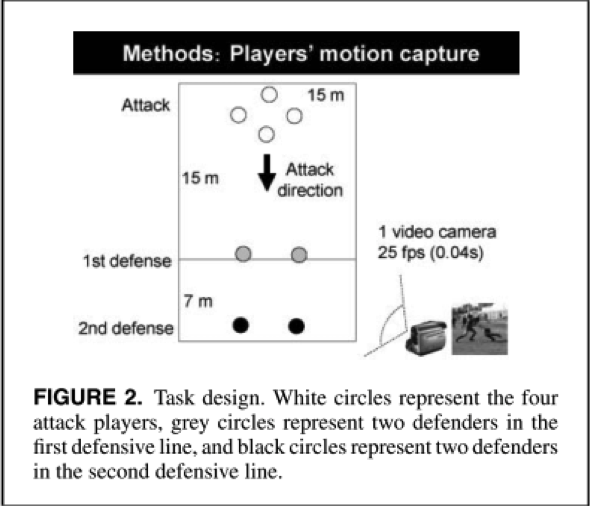
\includegraphics[width = \linewidth]{/Users/jacob1/Documents/2017/Research/DPhil/Dissertation/finalDocuments/jointActionSocialBonding/images/invasionDrill.png}
  \caption{The Invasion Drill from Passos (2011)}
  \label{fig:invasionDrill}
\end{figure}

\subsubsection{Experimental Paradigm: Invasion Drill}
This study required athletes to participate in a common rugby training drill, which was preceeded by one of two experimental primes—--a ``high difficulty'' condition, or a ``low difficulty'' condition.   Replicating \textcite{Passos2011}, a common training drill known as ``invasion drill'' \citep{Biscombe1998} was selected as it was representative of a typical subphase of rugby union.  In this drill a group of four rugby players formed an attacking group and two pairs of opponents formed a first and second defensive line.  There were two performance aims of this drill: (a) attackers were asked carry the ball into the try area, and (b) defenders were asked to stop the attacker’s progression toward the try line.  One trial consisted of one attempt by the attacking sub-group to penetrate two defending sub-groups, and carry the ball over the try line. The drill was conducted on a regulation multipurpose 110m x 70m grass or artificial turf training field within a 22m x 15m rectangle area marked by plastic cones (see ~\ref{fig:invasionDrill}). The ball used was size 5, as recommended by World Rugby for this age group of athletes.

%The training drill, known as ``invasion drill,'' requires eight athletes, one sub-grouof four attackers and two sub-groups of two defenders.  The primary aim of the drill is for the sub-group of 4 attacking players to successfully penetrate two consecutive lines of two defenders (also commonly known as a ``4 on 2 + 2'' drill). The aim of the two defending sub-groups is to stop the attacking team from achieving the primary goal, by interfering with their coordination by halting the ball-carrier, or the ball in flight between attacking players.




\subsubsection{Experimental Conditions: high and low difficulty}

Two different pre-experiment introductions were developed for the same training drill in order to manipulate athletes’ expectations around the technical difficulty of the impending joint-action task.  Athletes in the ``high difficulty'' condition learned that the overall average difficulty rating for the training drill provided by World Rugby coaches and athletes was 77.5/100, or approximately 8 out of 10.  Athletes were told that the drill would require an extension of their abilities as individuals and as a training group (see appendix for full script).  Athletes in the ``low difficulty'' condition, by contrast, learned that they would be participating in an ostensibly different drill with an overall average difficulty rating (provided by World Rugby coaches and athletes) of 22.5/100, or approximately 2 out of 10.  In reality, the training drill was exactly the same for each experimental session, and the relative difficulty of this drill was estimated in a pilot study to be approximately 5/10, see APPENDIX).  By either over- or under-rating the difficulty of the impending training drill, it was hoped that athletes' expectations around certainty of performance would be altered, such that athletes in the high difficulty condition would experience on average higher positive violation of expectations around team performance, whereas athletes in the low difficulty condition would experience less positive violations of expectations around team performance.


\subsubsection{Surveys}
Athletes completed survey questionnaires via WeChat using their personal mobile devices and internet connection. Surveys were administered at three time points: 1) one day before the experiment (Baseline), 2) immediately before the experiment after receiving the experimental prime (Pre-Experiment), and 3) once immediately following the completion of the experiment (Post-Experiment)(see TABLE).  At time 1 (baseline) athletes were asked about their impressions of recent individual performance and the performance of their procinvial team, including their feelings of team click and social bonding with their provincial team as a whole.  At time 2 (post-manipulation, pre-experiment), athletes were asked questions about their expectations concerning their individual performance and the performance of their specific training group in the impending training drill.  At time 3 (post-experiment), athletes completed questions concerning their impression of their own performance and the performance of their specific training group in the training drill. In addition, athletes were also asked about their feelings of team click and social bonding to the team as a whole (the same set of items that were asked one day earlier at time 1 (Baseline)).

\subsubsection{Survey Items}

The survey at time 1 (baseline) including items regarding recent individual and team performance, subjective and objective measures of technical competence in rugby, perceptions of team click, and social bonding to the team as a whole.  In addition, the time 1 survey also included items concerning basic personal information, current injury status, and personality type.

%survey items included questions regarding individual and team performance, including how athletes felt about their 1) overall individual performance, 2) specific components of individual performance (passing technique, support play in attack, 1on1 defense, effectiveness in contact, and decision making in game-play), 3) overall team performance and 4) specific components of team perfomance (coordination of the defensive line and attacking line, support play, and onfield communication) throughout the past month of training and competition.  All these items were recorded on a 100 point scale, 0 - ``Extremely poor'', 100 - ``Extremely good.''  Athletes were also asked about their individual technical competence relative to teammates and other Chinese and international athletes, as well perceived competence of their team relative to other Chinese provincial teams.
%Athletes were also asked if their perception of recent performance influences their 1) mood and 2) confidence regarding future performance (All these items were measured with a zero-centred 100 point scale, -50 - ``Extremely weak'', 0 - ``Average'', 50 - ``Extremely strong'').

%Athletes were also asked about their feelings concerning team click over the past month.  These items included: feelings about the unspoken understanding between athletes, the general atmosphere of the team (100 point scale, 0 - ``Extremely poor'', 100 - ``Extremely strong''), the extent to which they agree that their on-field abilities have been extended by other athletes (100 point scale, 0 - ``Completely disagree'', 100 - ``Completely agree''), and the reliability of other athletes to perform on-field roles and their own reliability in performing on-field roles for other athletes (100 point scale, 0 - ``Extremely unreliable'', 100 - ``Extremely reliable''), and a pictorial ``team click" measure (a visual item with five responses, ranging from less to more coordinated arrangements of dots (representing 12 athletes in a sevens tournament squad).
%In addition, athletes were asked about their feelings regarding their team's commitment to aspects of discipline over the past month (punctuality, observing bed times and curfews, attendance at meals, general team conduct) (100 point scale, 0 - ``Extremely poor'', 100 - ``Extremely strong'')).

%Athletes were asked about their feelings of social bonding to their team over the past month, including perceived emotional support and shared goal (100 point scale, 0 - ``Exrtremely weak'', 100 - ``Extremely strong''), identity fusion (pictorial scale and 7 item verbal scale, see APPENDIX), and group identification (six-item scale, see APPENDIX). In addition, athletes were also asked about identity fusion to country and family, measured using the pictorial fusion scale, and were then asked to rank their level of fusion to team, country, and family in order of most fused to least fused.  Athletes were also asked about their personality type using a common ten-item personality measure \citep[Ten Item Personality Index - TIPI][see APPENDIX]{Gosling2003}.

The survey administered at time 2, following the experimental manipulation and immediately prior to the experimnent, was designed to measure athletes' expectations regarding individual and group performance in light of the experimental prime. It also included items designed to measure athletes' perceptions of team click and social bonding to the training group (but not the team as a whole beyond the immediate training group).
In addition to these items, the time 2 survey also asked about current injury status, and state of arousal and fatigue (see APPENDIX for full details).

The final survey, administered at time 3 immediately post-experiment, consisted of items designed to assess athlete perceptions of individual and group performance in the experiment relative to prior expectations, as well as feelings of team click and social bonding to the training group. In addition to items already described above, athletes were asked if they would prefer to stay with their existing group or change to a new group for subsequent training experiments.  In addition to these group-specific items, the time 3 survey also included items regarding social bonding to the team as a whole (beyond an athlete's specific training group), in order to assess any change in these measures due to their experience of joint action in the experiment.  Finally, the time 3 survey also asked about current injury status and state of arousal and fatigue (see APPENDIX for full details).

\subsubsection{Video Analysis}
In order to produce quantitative measures of interpersonal coordination between co-actors, athletes’ motion was captured by a single digital video camera (Sony FDR-AX700 4K HDR Camcorder) mounted on a 1.2m high tripod. Digital video images of action were acquired by a computer, using a USB2.0 cable, and files were saved on an encrypted external hard disk in .AVI format. For image treatment, TACTO 8.0 software was used for digitizing at 25 frames per second.

\subsection{Design}
A between-subjects experimental design was used, in which expectations of technical difficulty was manipulated in one of two conditions, ``high difficulty'' and ``low difficulty'' condition.  Surveys measuring athletes' perceptions of joint action success, team click, and feelings of social bonding to the specific training group and the entire provincial team were recorded both before and after the experiment.

%The design of a study is its overall structure. What were the independent and dependent variables? Was the independent variable manipulated, and if so, was it manipulated between or within subjects? How were the variables operationally defined?

\subsection{Proceedure}
Permission to run the study was sought from the head coach of each of the four teams (Beijing men's, Beijing women's, Shandong men's, Shandong women's).  These coaches nominated athletes who were fit and able to complete the session without compromising their existing training schedules.  Athletes were randomly assigned to one of two conditions, and athletes in each condition were matched as much as possible according to average training age.

Once athletes were assigned to an experimental group, they were then added to a WeChat group populated by other training group members and the researcher. Atheltes were provided with the initial cover story for the experiment via ths WeChat group.  Athletes were told that the aim of the researcher was to trial a number of different rugby training drills selected from a recent report by World Rugby concerning training methods for rugby sevens.  These training drills had been previously rated by a selection of international level coaches and players from all over the world (including Asia and China), and the researcher planned to assess these ratings by testing by analysing how athletes react physiologically and psychologically to the demands of each drill.  Athletes were informed that data would be collected in the form of pre- and post-experiment surveys and video footage of the training drill (for full script, see APPENDIX).

Approximately 24 hours before the each experiment, athletes were instructed to complete the baseline survey by openning a link provided in the WeChat group.  This survey included written consent for the study. Approximately 1 hour before the experiment was due to take place, athletes were administered with an experimental prime via Wechat.  In the ``high difficulty'' condition, athletes were primed to believe that they were about to participate in a very difficult training drill (on the upper end of their individual and gorup technical abilities), whereas athletes in the ``low difficulty'' condition were primed to believe that they were about to participate in an easy training drill well within their tehcnical abilities (see APPENDIX for full script). All athletes were lead to believe that athletes in the other experiemntal groups were performing different drills to their assigned drill. (In reality, the training drill for each condition was identical, the only thing that varied was the pre-experiment prime).

Once athletes were assembled at the designated training field, the difficulty prime that had been sent via WeChat an hour earlier was verbally re-administered to the athletes. In addition, athletes were told in more detail about the requirements of the Invasion Drill (see APPENDIX for full details).  Athletes were told that assessment of performance in the experiment would be based on video analysis of an individual's performance in attack and defense, including an athlete's ability to coordinate attack and defense with others. Besides this outcome, athletes were provided with no other explicit information regarding performance goals, besides completing the experimental drill to the best of their ability within the rules of rugby union.

Athletes were then administered with the time 2 survey (pre-experiment, post-manipulation), which took approximately 3-5 minutes to complete.  After every athlete had finished the survey, athletes participated in a ~10 minute standard warm up routine, including slow jogging and dynamic stretching.  Athletes were instructed not to use the rugby ball during this period.  Once atheltes had completed the warm up, the researcher assembled the group within the training drill area, with one athlete standing on each of the 8 available plastic markers.  In this position, athletes were told once more about the structure and procedure for the training drill, in particular the way in which athletes were expected to rotate clockwise after every trial of the drill so that athletes did not habituate to certain positions or alliances in the drill (see fig Passos 2nd picture).

To begin the drill, the ball-carier at the front and centre of the attack sub-group was instructed to tap the ball with his / her foot, before initiating the attacking sub-phase by advancing forward towards the defence sub-units.  In the case that the ball was immediately fumbled during the inition of the trial, the training group was instructed to restart that trial and the trial in which the mistake was made was not counted.  Following a block of 4 practice trials, athletes were told by the researcher that the formal test was beginning. The group of athletes then completed 16 trials of the drill, which allowed each athlete to complete four trials of attack and four trials of defence, in different positions.  Following completion of all 16 test trials, athletes were assembled by the researcher and thanked for their participation, before being sent the sideline to complete the final post-experiment survey on their mobile devices.  Following the completion of this final survey, athletes were told that they would be informed within two days about the next experiment trial (in fact no more experiments were taking place).

In the case that athletes were unable to participate in their assigned condition for reasons of injury (2), a dummy athlete naive to the details of the study was used to fill in as part of the 8 person drill.  In the two experimental conditions involving the Beijing women's team, two athletes each session were unable to complete the experiment due to injury and sickness, and as such the drill was modified to a 3 on 2 + 1 Invasion drill requiring only 6 athletes, instead of the 4 on 2 + 2 drill, which requied 8.


\myparagraph{Video Analysis Procedure}
The digital camera and tripod were positioned on a platform 2m above the level of the playing field, approximately 10-15m from the bottom try-line corner of the Invasion Drill perimeter (see figure ~\ref{fig:invasionDrill}).  The experimenter began video recording before the athletes arrived, and ceased recording after all athletes had left the training field following the experiment.  Digital video images of action were acquired by a computer, using a USB2.0 cable, and files were saved on an encrypted external hard disk in .AVI format. For image treatment, TACTO 8.0 software was used for digitizing at 25 frames per second.

%The procedure is how the study was carried out. It often works well to describe the procedure in terms of what the participants did rather than what the researchers did. For example, the participants gave their informed consent, read a set of instructions, completed a block of four practice trials, completed a block of 20 test trials, completed two questionnaires, and were debriefed and excused.




\section{Results}

A total of 58 athletes participated in 8 experimental sessions. In one session (Shandong men's high difficulty condition) a dummy participant stood in for an athlete could not participate due to injury.  In the two sessions with Beijing women's team, due to failure of athletes to take part due to injury (3) or illness (2) the training drill was modfied to a ``3 on 2 + 1'' drill, requiring only 6 athletes to complete. In one of these experimental sessions, a female dummy participant was also required to fill in to make up a total of 6 athletes for the modified drill.  In both cases, dummy participants were competent ex-athletes naive to the predictions of the study and they did not participate in the survey responses before or after the session.  The survey and video data of the remaining 58 athletes were analysed.

\subsection{Survey Data}

\begin{knitrout}
\definecolor{shadecolor}{rgb}{0.969, 0.969, 0.969}\color{fgcolor}\begin{kframe}


{\ttfamily\noindent\color{warningcolor}{\#\# Warning: package 'dplyr' was built under R version 3.3.2}}

{\ttfamily\noindent\itshape\color{messagecolor}{\#\# \\\#\# Attaching package: 'dplyr'}}

{\ttfamily\noindent\itshape\color{messagecolor}{\#\# The following objects are masked from 'package:stats':\\\#\# \\\#\#\ \ \ \  filter, lag}}

{\ttfamily\noindent\itshape\color{messagecolor}{\#\# The following objects are masked from 'package:base':\\\#\# \\\#\#\ \ \ \  intersect, setdiff, setequal, union}}\end{kframe}
\end{knitrout}

% latex table generated in R 3.3.0 by xtable 1.8-2 package
% Mon Oct  9 11:36:23 2017
\begin{table}[ht]
\centering
\begin{tabular}{rl}
  \hline
 & Overall \\ 
  \hline
n &    58 \\ 
  Age (mean (sd)) & 21.33 (3.33) \\ 
  Sex = male (\%) &    31 (53.4)  \\ 
  Team (\%) &     \\ 
     Beijing Men &    16 (27.6)  \\ 
     Beijing Women &    11 (19.0)  \\ 
     Shandong Men &    15 (25.9)  \\ 
     Shandong Women &    16 (27.6)  \\ 
  Position = Starting Team (\%) &    18 (32.7)  \\ 
  TrainingAge (mean (sd)) &  4.22 (2.11) \\ 
  YearsInTeam (mean (sd)) &  5.64 (2.08) \\ 
  AthleteLevel (\%) &     \\ 
     1st Level &    11 (20.8)  \\ 
     2nd Level &     6 (11.3)  \\ 
     Master &    36 (67.9)  \\ 
  ContractStatus (\%) &     \\ 
     Full time contract &     8 (14.5)  \\ 
     Full time employee &    21 (38.2)  \\ 
     Student contract &     8 (14.5)  \\ 
     Training contract &    16 (29.1)  \\ 
     Trial &     2 ( 3.6)  \\ 
   \hline
\end{tabular}
\caption{Overview of experiment sample} 
\label{tab:athleteDescriptivesTraining}
\end{table}

% latex table generated in R 3.3.0 by xtable 1.8-2 package
% Wed Oct 11 15:23:43 2017
\begin{table}[ht]
\centering
\begin{tabular}{rll}
  \hline
 & low & high \\ 
  \hline
n &    29 &    29 \\ 
  Age (mean (sd)) & 22.14 (3.39) & 20.48 (3.11) \\ 
  Sex = male (\%) &    16 (55.2)  &    15 (51.7)  \\ 
  Team (\%) &     &     \\ 
     Beijing Men &     8 (27.6)  &     8 (27.6)  \\ 
     Beijing Women &     5 (17.2)  &     6 (20.7)  \\ 
     Shandong Men &     8 (27.6)  &     7 (24.1)  \\ 
     Shandong Women &     8 (27.6)  &     8 (27.6)  \\ 
  Position = Starting Team (\%) &     9 (32.1)  &     9 (33.3)  \\ 
  TrainingAge (mean (sd)) &  4.68 (2.25) &  3.74 (1.89) \\ 
  YearsInTeam (mean (sd)) &  5.89 (2.20) &  5.37 (1.94) \\ 
  AthleteLevel (\%) &     &     \\ 
     1st Level &     6 (22.2)  &     5 (19.2)  \\ 
     2nd Level &     1 ( 3.7)  &     5 (19.2)  \\ 
     Master &    20 (74.1)  &    16 (61.5)  \\ 
  ContractStatus (\%) &     &     \\ 
     Full time contract &     5 (17.9)  &     3 (11.1)  \\ 
     Full time employee &    11 (39.3)  &    10 (37.0)  \\ 
     Student contract &     3 (10.7)  &     5 (18.5)  \\ 
     Training contract &     8 (28.6)  &     8 (29.6)  \\ 
     Trial &     1 ( 3.6)  &     1 ( 3.7)  \\ 
   \hline
\end{tabular}
\caption{Overview of experiment sample by condition} 
\label{tab:athleteDescriptivesConditionTraining}
\end{table}



The attributes of the overall sample of athletes are displayed in Table ~\ref{tab:athleteDescriptivesTraining}. The average training age of athletes was 4.2181818 years (2.1142454), with athletes having spent on average over 6 years in the team. 36\% of the sample were full-time employees of their provincial team, with the rest either being employed on a full-time (but fixed term) contract
(800\%)), a ``student contract'' ((1600\%))), a short term training contract
((800\%))), or on a short-term trial basis ((200\%))).  Only 18 of 58 (31\%) of athletes declared that there were in the starting team of their respective provincial teams.  Attributes of athletes in the high and low difficulty conditions were evenly matched (see Table ~\ref{tab:athleteDescriptivesConditionTraining}), with only a marginally significant difference in average age between conditions (high difficulty condition = 20.4814815(3.1054588), low difficulty condition = 22.1428571(3.3853091).




The central tendencies of subjective measures of individual technical competence compared to teammates, other Chinese professional rugby players, and International professionals, were all above the mid-point of the zero-centred scale (min = -50, max = 50, see Table ~\ref{tab:compPerfSubjTraining}).  The central tendencies for items concerning the impact of individual performance on mood and confidence were also well above the mid-point of the scale (100 point scale, min = 0, max = 100). Likewise, average athlete perceptions of individual (Tables ~\ref{tab:indPerfTimeLowTraining} and ~\ref{tab:indPerfTimeHighTraining}), group (Tables ~\ref{tab:groupPerfTimeLowTraining} and ~\ref{tab:groupPerfTimeHighTraining}), and team (measured at Baseline only, see Table ~\ref{tab:teamPerfTimeBaselineTraining}) performance were above the mid-point of the scale for both conditions at all time points.
Variables measuring athletes' perceptions of group and team click, and feelings of bonding to the training group and the team as a whole also showed high negative skew above the mid-point of each respective scale (see Tables ~\ref{tab:groupClickTimeHighTraining}\nobreakdash--\ref{tab:teamBondingTimeHighTraining}).


%Among these measures, perceived technical competence relative to international rugby players differed significantly by cont

%% latex table generated in R 3.3.0 by xtable 1.8-2 package
% Wed Oct 11 15:28:37 2017
\begin{table}[ht]
\centering
\begin{tabular}{rll}
  \hline
 & high & low \\ 
  \hline
n &    87 &    87 \\ 
  CompetenceVsTeammates (mean (sd)) & 25.41 (15.49) & 22.52 (16.46) \\ 
  CompetenceVsChinesePros (mean (sd)) & 16.89 (19.39) & 17.30 (17.69) \\ 
  CompetenceVsInternationalPros (mean (sd)) & 24.85 (24.52) & 14.11 (26.88) \\ 
  PerfomanceImpactOnConfidence (mean (sd)) & 68.00 (23.06) & 69.26 (24.80) \\ 
  PerformanceImpactOnMood (mean (sd)) & 67.70 (23.78) & 66.89 (16.21) \\ 
   \hline
\end{tabular}
\caption{Athlete subjective perceptions of 
 individual technical competence by condition} 
\label{tab:indPerfTimeHighTraining}
\end{table}

%%IndPerforamnce:
%% latex table generated in R 3.5.0 by xtable 1.8-2 package
% Mon Aug 27 19:27:20 2018
\begin{table}[ht]
\centering
\begin{tabular}{rlll}
  \hline
 & Baseline & Pre & Post \\ 
  \hline
n &    29 &    29 &    29 \\ 
  PerformanceVsExpectations (mean (sd)) &   NaN (NA) &   NaN (NA) & 44.41 (26.83) \\ 
  ConfidenceInAbility (mean (sd)) &   NaN (NA) & 77.76 (15.37) & 68.93 (24.87) \\ 
  Defence (mean (sd)) & 60.96 (19.16) & 63.62 (19.56) & 58.69 (23.58) \\ 
  Passing (mean (sd)) & 61.74 (22.23) & 70.28 (16.21) & 60.21 (22.78) \\ 
  SupportPlay (mean (sd)) & 69.19 (14.23) & 70.31 (15.79) & 67.62 (23.05) \\ 
  DecisionMaking (mean (sd)) & 59.89 (16.76) & 62.93 (16.89) & 68.21 (14.68) \\ 
  OverallPerformance (mean (sd)) & 66.11 (19.47) & 69.90 (17.35) &   NaN (NA) \\ 
   \hline
\end{tabular}
\caption{Athlete perceptions of 
 individual performance (low difficulty condition)} 
\label{tab:indPerfTimeHighTraining}
\end{table}

%% latex table generated in R 3.3.0 by xtable 1.8-2 package
% Mon Oct 16 10:48:01 2017
\begin{table}[ht]
\centering
\begin{tabular}{rlll}
  \hline
 & Baseline & Pre & Post \\ 
  \hline
n &    29 &    29 &    29 \\ 
  PerformanceVsExpectations (mean (sd)) &   NaN (NA) &   NaN (NA) & 64.79 (16.83) \\ 
  ConfidenceInAbility (mean (sd)) &   NaN (NA) & 76.90 (22.65) & 73.32 (14.03) \\ 
  Defence (mean (sd)) & 67.44 (16.83) & 66.76 (19.68) & 66.11 (16.67) \\ 
  Passing (mean (sd)) & 63.63 (26.69) & 65.83 (20.93) & 59.75 (24.52) \\ 
  SupportPlay (mean (sd)) & 67.30 (24.88) & 67.90 (23.13) & 66.61 (21.35) \\ 
  DecisionMaking (mean (sd)) & 60.78 (23.72) & 65.93 (20.43) & 67.11 (21.70) \\ 
  OverallPerformance (mean (sd)) & 69.07 (18.62) & 65.66 (27.57) &   NaN (NA) \\ 
   \hline
\end{tabular}
\caption{Athlete perceptions of 
 individual performance (high difficulty condition)} 
\label{tab:indPerfTimeHighTraining}
\end{table}

%% groupPerformance:
%% latex table generated in R 3.3.0 by xtable 1.8-2 package
% Mon Oct  9 11:36:24 2017
\begin{table}[ht]
\centering
\begin{tabular}{rlllll}
  \hline
 & Baseline & Pre & Post & p & test \\ 
  \hline
n &  29 &    29 &    29 &  &  \\ 
  ConfidenceInGroupAbility (mean (sd)) & NaN (NA) & 78.62 (12.75) &   NaN (NA) &  NA &  \\ 
  GroupAttack (mean (sd)) & NaN (NA) & 75.66 (13.36) & 67.34 (15.61) &  0.034 &  \\ 
  GroupDefence (mean (sd)) & NaN (NA) & 77.62 (14.44) & 63.14 (19.90) &  0.002 &  \\ 
  GroupCommunication (mean (sd)) & NaN (NA) & 75.72 (14.84) & 70.66 (15.46) &  0.208 &  \\ 
  GroupSupportPlay (mean (sd)) & NaN (NA) & 75.97 (12.80) & 69.66 (13.72) &  0.076 &  \\ 
   \hline
\end{tabular}
\caption{Athlete perceptions of 
 group performance (low difficulty condition)} 
\end{table}

%% latex table generated in R 3.3.0 by xtable 1.8-2 package
% Mon Oct 16 10:48:01 2017
\begin{table}[ht]
\centering
\begin{tabular}{rlll}
  \hline
 & Baseline & Pre & Post \\ 
  \hline
n &  29 &    29 &    29 \\ 
  ConfidenceInGroupAbility (mean (sd)) & NaN (NA) & 76.03 (17.16) &   NaN (NA) \\ 
  GroupAttack (mean (sd)) & NaN (NA) & 74.55 (20.93) & 64.07 (24.38) \\ 
  GroupDefence (mean (sd)) & NaN (NA) & 73.38 (22.09) & 57.04 (25.55) \\ 
  GroupCommunication (mean (sd)) & NaN (NA) & 77.76 (16.09) & 66.25 (20.78) \\ 
  GroupSupportPlay (mean (sd)) & NaN (NA) & 75.55 (15.65) & 64.46 (25.32) \\ 
   \hline
\end{tabular}
\caption{Athlete perceptions of 
 group performance (high difficulty condition)} 
\end{table}

%% teamPerformance:
%% latex table generated in R 3.3.0 by xtable 1.8-2 package
% Wed Oct 11 10:01:30 2017
\begin{table}[ht]
\centering
\begin{tabular}{rllll}
  \hline
 & high & low & p & test \\ 
  \hline
n &    87 &    87 &  &  \\ 
  TeamPerformance (mean (sd)) & 69.96 (19.74) & 68.00 (23.11) &  0.739 &  \\ 
  TeamCompetenceInChina (mean (sd)) & 37.81 (16.08) & 41.19 (13.43) &  0.407 &  \\ 
  TeamAttack (mean (sd)) & 65.74 (24.68) & 66.85 (15.07) &  0.843 &  \\ 
  TeamDefence (mean (sd)) & 67.30 (16.99) & 63.26 (17.79) &  0.398 &  \\ 
  TeamCommunication (mean (sd)) & 70.67 (19.48) & 65.67 (22.27) &  0.384 &  \\ 
  TeamSupportPlay (mean (sd)) & 68.11 (18.61) & 64.15 (19.15) &  0.444 &  \\ 
   \hline
\end{tabular}
\caption{Athlete perceptions of team performance 
 at Baseline, by condition} 
\label{tab:teamPerfBaselineTraining}
\end{table}

%% groupClick:
%% latex table generated in R 3.3.0 by xtable 1.8-2 package
% Mon Oct  9 11:36:24 2017
\begin{table}[ht]
\centering
\begin{tabular}{rlllll}
  \hline
 & Baseline & Pre & Post & p & test \\ 
  \hline
n &  29 &    29 &    29 &  &  \\ 
  ClickPictorial (mean (sd)) & NaN (NA) &  4.00 (0.89) &  3.75 (0.93) &  0.303 &  \\ 
  UnspokenUnderstanding (mean (sd)) & NaN (NA) & 72.90 (15.77) & 64.64 (20.99) &  0.098 &  \\ 
  GeneralAtmosphere (mean (sd)) & NaN (NA) & 78.03 (17.48) & 74.50 (20.54) &  0.487 &  \\ 
  AbilitiesExtended (mean (sd)) & NaN (NA) & 72.28 (16.22) & 61.86 (28.68) &  0.096 &  \\ 
  ReliabilityForOthers (mean (sd)) & NaN (NA) &   NaN (NA) & 63.46 (14.56) &  NA &  \\ 
  ReliabilityOfOthers (mean (sd)) & NaN (NA) &   NaN (NA) & 72.29 (17.79) &  NA &  \\ 
   \hline
\end{tabular}
\caption{Athlete perceptions of 
 group click (high difficulty condition)} 
\end{table}

%% latex table generated in R 3.3.0 by xtable 1.8-2 package
% Mon Oct  9 11:36:24 2017
\begin{table}[ht]
\centering
\begin{tabular}{rlllll}
  \hline
 & Baseline & Pre & Post & p & test \\ 
  \hline
n &  29 &    29 &    29 &  &  \\ 
  ClickPictorial (mean (sd)) & NaN (NA) &  3.76 (1.18) &  3.45 (1.24) &  0.334 &  \\ 
  UnspokenUnderstanding (mean (sd)) & NaN (NA) & 72.45 (19.40) & 68.34 (14.69) &  0.368 &  \\ 
  GeneralAtmosphere (mean (sd)) & NaN (NA) & 81.79 (11.60) & 76.79 (13.73) &  0.140 &  \\ 
  AbilitiesExtended (mean (sd)) & NaN (NA) & 77.66 (14.33) & 65.86 (18.09) &  0.008 &  \\ 
  ReliabilityForOthers (mean (sd)) & NaN (NA) &   NaN (NA) & 61.03 (21.33) &  NA &  \\ 
  ReliabilityOfOthers (mean (sd)) & NaN (NA) &   NaN (NA) & 68.55 (23.47) &  NA &  \\ 
   \hline
\end{tabular}
\caption{Athlete perceptions of 
 group click (low difficulty condition)} 
\end{table}

%% groupBonding:
%% latex table generated in R 3.3.0 by xtable 1.8-2 package
% Mon Oct  9 11:36:24 2017
\begin{table}[ht]
\centering
\begin{tabular}{rlllll}
  \hline
 & Baseline & Pre & Post & p & test \\ 
  \hline
n &  29 &    29 &    29 &  &  \\ 
  EmotionalSupport (mean (sd)) & NaN (NA) & 78.55 (18.90) & 73.86 (19.61) &  0.361 &  \\ 
  SharedGoal (mean (sd)) & NaN (NA) & 80.79 (24.98) & 79.04 (20.80) &  0.774 &  \\ 
  FusionPictorial (mean (sd)) & NaN (NA) &  4.14 (0.64) &  4.00 (1.09) &  0.560 &  \\ 
  StayOrChange (mean (sd)) & NaN (NA) &   NaN (NA) & 68.25 (24.75) &  NA &  \\ 
   \hline
\end{tabular}
\caption{Athlete perceptions of 
 group bonding (high difficulty condition)} 
\end{table}

%% latex table generated in R 3.5.0 by xtable 1.8-2 package
% Mon Aug 27 19:27:21 2018
\begin{table}[ht]
\centering
\begin{tabular}{rlll}
  \hline
 & Baseline & Pre & Post \\ 
  \hline
n &  29 &    29 &    29 \\ 
  EmotionalSupport (mean (sd)) & NaN (NA) & 78.69 (24.33) & 76.52 (14.92) \\ 
  SharedGoal (mean (sd)) & NaN (NA) & 90.21 (9.33) & 83.62 (15.34) \\ 
  FusionPictorial (mean (sd)) & NaN (NA) &  4.31 (0.71) &  3.79 (1.52) \\ 
  StayOrChange (mean (sd)) & NaN (NA) &   NaN (NA) & 71.79 (24.23) \\ 
   \hline
\end{tabular}
\caption{Athlete perceptions of 
 group bonding (low difficulty condition)} 
\end{table}

%% teamBonding:
%% latex table generated in R 3.3.0 by xtable 1.8-2 package
% Mon Oct  9 11:36:25 2017
\begin{table}[ht]
\centering
\begin{tabular}{rlllll}
  \hline
 & Baseline & Pre & Post & p & test \\ 
  \hline
n &    29 &  29 &    29 &  &  \\ 
  EmotionalSupport (mean (sd)) & 77.11 (17.76) & NaN (NA) & 76.90 (11.97) &  0.958 &  \\ 
  SharedGoal (mean (sd)) & 84.96 (16.93) & NaN (NA) & 84.28 (14.13) &  0.869 &  \\ 
  FusionVerbalTeam (mean (sd)) &  4.15 (0.65) & NaN (NA) &  4.06 (0.61) &  0.595 &  \\ 
  GroupIdentification (mean (sd)) &  4.49 (0.57) & NaN (NA) &  4.40 (0.64) &  0.568 &  \\ 
  FusionPictorialTeam (mean (sd)) &  4.67 (0.48) & NaN (NA) &  4.45 (0.63) &  0.153 &  \\ 
  FusionPictorialFamily (mean (sd)) &  4.52 (1.09) & NaN (NA) &  4.69 (0.71) &  0.486 &  \\ 
  FusionPictorialCountry (mean (sd)) &  4.00 (1.33) & NaN (NA) &  3.93 (1.36) &  0.849 &  \\ 
  TeamRank (mean (sd)) &  1.33 (0.68) & NaN (NA) &  1.28 (0.70) &  0.757 &  \\ 
  FamilyRank (mean (sd)) &  1.56 (0.85) & NaN (NA) &  1.69 (0.81) &  0.547 &  \\ 
  CountryRank (mean (sd)) &  0.56 (1.01) & NaN (NA) &  0.59 (1.05) &  0.912 &  \\ 
   \hline
\end{tabular}
\caption{Athlete perceptions of 
 team bonding (low difficulty condition)} 
\end{table}

%% latex table generated in R 3.5.0 by xtable 1.8-2 package
% Mon Aug 27 19:27:21 2018
\begin{table}[ht]
\centering
\begin{tabular}{rlll}
  \hline
 & Baseline & Pre & Post \\ 
  \hline
n &    29 &  29 &    29 \\ 
  EmotionalSupport (mean (sd)) & 71.89 (24.66) & NaN (NA) & 71.71 (17.46) \\ 
  SharedGoal (mean (sd)) & 81.59 (17.66) & NaN (NA) & 82.64 (17.18) \\ 
  FusionVerbalTeam (mean (sd)) &  4.00 (0.81) & NaN (NA) &  3.88 (0.76) \\ 
  GroupIdentification (mean (sd)) &  4.20 (0.78) & NaN (NA) &  4.16 (0.71) \\ 
  FusionPictorialTeam (mean (sd)) &  4.33 (0.73) & NaN (NA) &  4.25 (0.75) \\ 
  FusionPictorialFamily (mean (sd)) &  4.56 (0.80) & NaN (NA) &  4.71 (0.71) \\ 
  FusionPictorialCountry (mean (sd)) &  3.56 (1.31) & NaN (NA) &  3.61 (1.57) \\ 
  TeamRank (mean (sd)) &  1.30 (0.78) & NaN (NA) &  1.25 (0.75) \\ 
  FamilyRank (mean (sd)) &  1.81 (0.74) & NaN (NA) &  1.75 (0.65) \\ 
  CountryRank (mean (sd)) &  0.56 (1.05) & NaN (NA) &  0.57 (1.00) \\ 
   \hline
\end{tabular}
\caption{Athlete perceptions of 
 team bonding (high difficulty condition)} 
\end{table}

%%teamDiscipline
%% latex table generated in R 3.3.0 by xtable 1.8-2 package
% Wed Oct 11 10:01:31 2017
\begin{table}[ht]
\centering
\begin{tabular}{rlllll}
  \hline
 & Baseline & Pre & Post & p & test \\ 
  \hline
n &    29 &  29 &    29 &  &  \\ 
  Punctuality (mean (sd)) & 87.33 (19.22) & NaN (NA) & 86.76 (19.33) &  0.912 &  \\ 
  MealAttendance (mean (sd)) & 92.78 (11.56) & NaN (NA) & 93.62 (9.48) &  0.766 &  \\ 
  GeneralConduct (mean (sd)) & 90.81 (11.68) & NaN (NA) & 92.86 (9.15) &  0.467 &  \\ 
  Curfew (mean (sd)) & 89.33 (19.39) & NaN (NA) & 89.34 (14.61) &  0.998 &  \\ 
   \hline
\end{tabular}
\caption{Athlete perceptions of 
 team discipine (low difficulty condition)} 
\end{table}

%%ArousalExertion:
%% latex table generated in R 3.5.0 by xtable 1.8-2 package
% Mon Aug 27 19:27:22 2018
\begin{table}[ht]
\centering
\begin{tabular}{rlll}
  \hline
 & Baseline & Pre & Post \\ 
  \hline
n &    29 &    29 &    29 \\ 
  Aroused (mean (sd)) &   NaN (NA) &  6.38 (2.82) &  8.00 (2.48) \\ 
  Excited (mean (sd)) &   NaN (NA) &  5.55 (2.68) &  7.31 (2.38) \\ 
  Relaxed (mean (sd)) &   NaN (NA) &  6.10 (3.04) &  8.14 (2.40) \\ 
  Fatigue (mean (sd)) &   NaN (NA) & 55.34 (22.14) & 40.93 (28.30) \\ 
  PhysicalExertion (mean (sd)) &   NaN (NA) &   NaN (NA) & 12.17 (2.99) \\ 
  MentalExertion (mean (sd)) &   NaN (NA) &   NaN (NA) &  3.38 (2.27) \\ 
  InjuryStatus (mean (sd)) & 85.37 (25.98) & 76.97 (24.47) & 75.76 (25.78) \\ 
   \hline
\end{tabular}
\caption{Athlete arousal and exertion 
 (low difficulty condition)} 
\end{table}

%%Personality:
%% latex table generated in R 3.3.0 by xtable 1.8-2 package
% Wed Oct 11 10:01:32 2017
\begin{table}[ht]
\centering
\begin{tabular}{rllll}
  \hline
 & high & low & p & test \\ 
  \hline
n &   87 &   87 &  &  \\ 
  Agreeableness (mean (sd)) & 4.94 (1.16) & 4.74 (0.93) &  0.481 &  \\ 
  Conscientiousness (mean (sd)) & 5.46 (1.18) & 5.20 (1.29) &  0.445 &  \\ 
  EmotionalStability (mean (sd)) & 4.26 (1.40) & 4.54 (1.42) &  0.472 &  \\ 
  Extraverted (mean (sd)) & 5.28 (1.44) & 4.74 (1.68) &  0.213 &  \\ 
  Openness (mean (sd)) & 4.62 (1.15) & 4.74 (0.97) &  0.679 &  \\ 
   \hline
\end{tabular}
\caption{Athlete personality type by condition} 
\end{table}




\subsubsection{Athlete perceptions of performance}

\myparagraph{Individual performance}
\begin{knitrout}
\definecolor{shadecolor}{rgb}{0.969, 0.969, 0.969}\color{fgcolor}\begin{kframe}


{\ttfamily\noindent\color{warningcolor}{\#\# Warning: package 'scales' was built under R version 3.3.2}}

{\ttfamily\noindent\color{warningcolor}{\#\# Warning in min(x, na.rm = TRUE): no non-missing arguments to min; returning Inf}}

{\ttfamily\noindent\color{warningcolor}{\#\# Warning in min(x, na.rm = TRUE): no non-missing arguments to min; returning Inf}}

{\ttfamily\noindent\color{warningcolor}{\#\# Warning in max(x, na.rm = TRUE): no non-missing arguments to max; returning -Inf}}

{\ttfamily\noindent\color{warningcolor}{\#\# Warning in max(x, na.rm = TRUE): no non-missing arguments to max; returning -Inf}}

{\ttfamily\noindent\color{warningcolor}{\#\# Warning in min(x, na.rm = TRUE): no non-missing arguments to min; returning Inf}}

{\ttfamily\noindent\color{warningcolor}{\#\# Warning in max(x, na.rm = TRUE): no non-missing arguments to max; returning -Inf}}

{\ttfamily\noindent\color{warningcolor}{\#\# Warning in min(x, na.rm = TRUE): no non-missing arguments to min; returning Inf}}

{\ttfamily\noindent\color{warningcolor}{\#\# Warning in max(x, na.rm = TRUE): no non-missing arguments to max; returning -Inf}}

{\ttfamily\noindent\color{warningcolor}{\#\# Warning in StdDiff(variable = var, group = strataVar): Variable has only NA's in at least one stratum. na.rm turned off.}}

{\ttfamily\noindent\color{warningcolor}{\#\# Warning in StdDiff(variable = var, group = strataVar): Variable has only NA's in at least one stratum. na.rm turned off.}}

{\ttfamily\noindent\color{warningcolor}{\#\# Warning in StdDiff(variable = var, group = strataVar): Variable has only NA's in at least one stratum. na.rm turned off.}}

{\ttfamily\noindent\color{warningcolor}{\#\# Warning in min(x, na.rm = TRUE): no non-missing arguments to min; returning Inf}}

{\ttfamily\noindent\color{warningcolor}{\#\# Warning in min(x, na.rm = TRUE): no non-missing arguments to min; returning Inf}}

{\ttfamily\noindent\color{warningcolor}{\#\# Warning in max(x, na.rm = TRUE): no non-missing arguments to max; returning -Inf}}

{\ttfamily\noindent\color{warningcolor}{\#\# Warning in max(x, na.rm = TRUE): no non-missing arguments to max; returning -Inf}}

{\ttfamily\noindent\color{warningcolor}{\#\# Warning in min(x, na.rm = TRUE): no non-missing arguments to min; returning Inf}}

{\ttfamily\noindent\color{warningcolor}{\#\# Warning in max(x, na.rm = TRUE): no non-missing arguments to max; returning -Inf}}

{\ttfamily\noindent\color{warningcolor}{\#\# Warning in min(x, na.rm = TRUE): no non-missing arguments to min; returning Inf}}

{\ttfamily\noindent\color{warningcolor}{\#\# Warning in max(x, na.rm = TRUE): no non-missing arguments to max; returning -Inf}}

{\ttfamily\noindent\color{warningcolor}{\#\# Warning in StdDiff(variable = var, group = strataVar): Variable has only NA's in at least one stratum. na.rm turned off.}}

{\ttfamily\noindent\color{warningcolor}{\#\# Warning in StdDiff(variable = var, group = strataVar): Variable has only NA's in at least one stratum. na.rm turned off.}}

{\ttfamily\noindent\color{warningcolor}{\#\# Warning in StdDiff(variable = var, group = strataVar): Variable has only NA's in at least one stratum. na.rm turned off.}}\end{kframe}
\end{knitrout}

% latex table generated in R 3.5.0 by xtable 1.8-2 package
% Mon Aug 27 19:27:20 2018
\begin{table}[ht]
\centering
\begin{tabular}{rlll}
  \hline
 & Baseline & Pre & Post \\ 
  \hline
n &    29 &    29 &    29 \\ 
  PerformanceVsExpectations (mean (sd)) &   NaN (NA) &   NaN (NA) & 44.41 (26.83) \\ 
  ConfidenceInAbility (mean (sd)) &   NaN (NA) & 77.76 (15.37) & 68.93 (24.87) \\ 
  Defence (mean (sd)) & 60.96 (19.16) & 63.62 (19.56) & 58.69 (23.58) \\ 
  Passing (mean (sd)) & 61.74 (22.23) & 70.28 (16.21) & 60.21 (22.78) \\ 
  SupportPlay (mean (sd)) & 69.19 (14.23) & 70.31 (15.79) & 67.62 (23.05) \\ 
  DecisionMaking (mean (sd)) & 59.89 (16.76) & 62.93 (16.89) & 68.21 (14.68) \\ 
  OverallPerformance (mean (sd)) & 66.11 (19.47) & 69.90 (17.35) &   NaN (NA) \\ 
   \hline
\end{tabular}
\caption{Athlete perceptions of 
 individual performance (low difficulty condition)} 
\label{tab:indPerfTimeHighTraining}
\end{table}

% latex table generated in R 3.3.0 by xtable 1.8-2 package
% Mon Oct 16 10:48:01 2017
\begin{table}[ht]
\centering
\begin{tabular}{rlll}
  \hline
 & Baseline & Pre & Post \\ 
  \hline
n &    29 &    29 &    29 \\ 
  PerformanceVsExpectations (mean (sd)) &   NaN (NA) &   NaN (NA) & 64.79 (16.83) \\ 
  ConfidenceInAbility (mean (sd)) &   NaN (NA) & 76.90 (22.65) & 73.32 (14.03) \\ 
  Defence (mean (sd)) & 67.44 (16.83) & 66.76 (19.68) & 66.11 (16.67) \\ 
  Passing (mean (sd)) & 63.63 (26.69) & 65.83 (20.93) & 59.75 (24.52) \\ 
  SupportPlay (mean (sd)) & 67.30 (24.88) & 67.90 (23.13) & 66.61 (21.35) \\ 
  DecisionMaking (mean (sd)) & 60.78 (23.72) & 65.93 (20.43) & 67.11 (21.70) \\ 
  OverallPerformance (mean (sd)) & 69.07 (18.62) & 65.66 (27.57) &   NaN (NA) \\ 
   \hline
\end{tabular}
\caption{Athlete perceptions of 
 individual performance (high difficulty condition)} 
\label{tab:indPerfTimeHighTraining}
\end{table}





\begin{knitrout}
\definecolor{shadecolor}{rgb}{0.969, 0.969, 0.969}\color{fgcolor}\begin{kframe}


{\ttfamily\noindent\color{warningcolor}{\#\# Warning in ModuleReturnVarsExist(vars, data): The data frame does not have: GroupPerformanceVsExpectations\ \ Dropped}}

{\ttfamily\noindent\color{warningcolor}{\#\# Warning in min(x, na.rm = TRUE): no non-missing arguments to min; returning Inf}}

{\ttfamily\noindent\color{warningcolor}{\#\# Warning in min(x, na.rm = TRUE): no non-missing arguments to min; returning Inf}}

{\ttfamily\noindent\color{warningcolor}{\#\# Warning in min(x, na.rm = TRUE): no non-missing arguments to min; returning Inf}}

{\ttfamily\noindent\color{warningcolor}{\#\# Warning in min(x, na.rm = TRUE): no non-missing arguments to min; returning Inf}}

{\ttfamily\noindent\color{warningcolor}{\#\# Warning in min(x, na.rm = TRUE): no non-missing arguments to min; returning Inf}}

{\ttfamily\noindent\color{warningcolor}{\#\# Warning in max(x, na.rm = TRUE): no non-missing arguments to max; returning -Inf}}

{\ttfamily\noindent\color{warningcolor}{\#\# Warning in max(x, na.rm = TRUE): no non-missing arguments to max; returning -Inf}}

{\ttfamily\noindent\color{warningcolor}{\#\# Warning in max(x, na.rm = TRUE): no non-missing arguments to max; returning -Inf}}

{\ttfamily\noindent\color{warningcolor}{\#\# Warning in max(x, na.rm = TRUE): no non-missing arguments to max; returning -Inf}}

{\ttfamily\noindent\color{warningcolor}{\#\# Warning in max(x, na.rm = TRUE): no non-missing arguments to max; returning -Inf}}

{\ttfamily\noindent\color{warningcolor}{\#\# Warning in min(x, na.rm = TRUE): no non-missing arguments to min; returning Inf}}

{\ttfamily\noindent\color{warningcolor}{\#\# Warning in max(x, na.rm = TRUE): no non-missing arguments to max; returning -Inf}}

{\ttfamily\noindent\color{warningcolor}{\#\# Warning in StdDiff(variable = var, group = strataVar): Variable has only NA's in at least one stratum. na.rm turned off.}}

{\ttfamily\noindent\color{warningcolor}{\#\# Warning in StdDiff(variable = var, group = strataVar): Variable has only NA's in at least one stratum. na.rm turned off.}}

{\ttfamily\noindent\color{warningcolor}{\#\# Warning in StdDiff(variable = var, group = strataVar): Variable has only NA's in at least one stratum. na.rm turned off.}}

{\ttfamily\noindent\color{warningcolor}{\#\# Warning in StdDiff(variable = var, group = strataVar): Variable has only NA's in at least one stratum. na.rm turned off.}}

{\ttfamily\noindent\color{warningcolor}{\#\# Warning in StdDiff(variable = var, group = strataVar): Variable has only NA's in at least one stratum. na.rm turned off.}}

{\ttfamily\noindent\color{warningcolor}{\#\# Warning in ModuleReturnVarsExist(vars, data): The data frame does not have: GroupPerformanceVsExpectations\ \ Dropped}}

{\ttfamily\noindent\color{warningcolor}{\#\# Warning in min(x, na.rm = TRUE): no non-missing arguments to min; returning Inf}}

{\ttfamily\noindent\color{warningcolor}{\#\# Warning in min(x, na.rm = TRUE): no non-missing arguments to min; returning Inf}}

{\ttfamily\noindent\color{warningcolor}{\#\# Warning in min(x, na.rm = TRUE): no non-missing arguments to min; returning Inf}}

{\ttfamily\noindent\color{warningcolor}{\#\# Warning in min(x, na.rm = TRUE): no non-missing arguments to min; returning Inf}}

{\ttfamily\noindent\color{warningcolor}{\#\# Warning in min(x, na.rm = TRUE): no non-missing arguments to min; returning Inf}}

{\ttfamily\noindent\color{warningcolor}{\#\# Warning in max(x, na.rm = TRUE): no non-missing arguments to max; returning -Inf}}

{\ttfamily\noindent\color{warningcolor}{\#\# Warning in max(x, na.rm = TRUE): no non-missing arguments to max; returning -Inf}}

{\ttfamily\noindent\color{warningcolor}{\#\# Warning in max(x, na.rm = TRUE): no non-missing arguments to max; returning -Inf}}

{\ttfamily\noindent\color{warningcolor}{\#\# Warning in max(x, na.rm = TRUE): no non-missing arguments to max; returning -Inf}}

{\ttfamily\noindent\color{warningcolor}{\#\# Warning in max(x, na.rm = TRUE): no non-missing arguments to max; returning -Inf}}

{\ttfamily\noindent\color{warningcolor}{\#\# Warning in min(x, na.rm = TRUE): no non-missing arguments to min; returning Inf}}

{\ttfamily\noindent\color{warningcolor}{\#\# Warning in max(x, na.rm = TRUE): no non-missing arguments to max; returning -Inf}}

{\ttfamily\noindent\color{warningcolor}{\#\# Warning in StdDiff(variable = var, group = strataVar): Variable has only NA's in at least one stratum. na.rm turned off.}}

{\ttfamily\noindent\color{warningcolor}{\#\# Warning in StdDiff(variable = var, group = strataVar): Variable has only NA's in at least one stratum. na.rm turned off.}}

{\ttfamily\noindent\color{warningcolor}{\#\# Warning in StdDiff(variable = var, group = strataVar): Variable has only NA's in at least one stratum. na.rm turned off.}}

{\ttfamily\noindent\color{warningcolor}{\#\# Warning in StdDiff(variable = var, group = strataVar): Variable has only NA's in at least one stratum. na.rm turned off.}}

{\ttfamily\noindent\color{warningcolor}{\#\# Warning in StdDiff(variable = var, group = strataVar): Variable has only NA's in at least one stratum. na.rm turned off.}}\end{kframe}
\end{knitrout}

% latex table generated in R 3.3.0 by xtable 1.8-2 package
% Mon Oct  9 11:36:24 2017
\begin{table}[ht]
\centering
\begin{tabular}{rlllll}
  \hline
 & Baseline & Pre & Post & p & test \\ 
  \hline
n &  29 &    29 &    29 &  &  \\ 
  ConfidenceInGroupAbility (mean (sd)) & NaN (NA) & 78.62 (12.75) &   NaN (NA) &  NA &  \\ 
  GroupAttack (mean (sd)) & NaN (NA) & 75.66 (13.36) & 67.34 (15.61) &  0.034 &  \\ 
  GroupDefence (mean (sd)) & NaN (NA) & 77.62 (14.44) & 63.14 (19.90) &  0.002 &  \\ 
  GroupCommunication (mean (sd)) & NaN (NA) & 75.72 (14.84) & 70.66 (15.46) &  0.208 &  \\ 
  GroupSupportPlay (mean (sd)) & NaN (NA) & 75.97 (12.80) & 69.66 (13.72) &  0.076 &  \\ 
   \hline
\end{tabular}
\caption{Athlete perceptions of 
 group performance (low difficulty condition)} 
\end{table}

% latex table generated in R 3.3.0 by xtable 1.8-2 package
% Mon Oct 16 10:48:01 2017
\begin{table}[ht]
\centering
\begin{tabular}{rlll}
  \hline
 & Baseline & Pre & Post \\ 
  \hline
n &  29 &    29 &    29 \\ 
  ConfidenceInGroupAbility (mean (sd)) & NaN (NA) & 76.03 (17.16) &   NaN (NA) \\ 
  GroupAttack (mean (sd)) & NaN (NA) & 74.55 (20.93) & 64.07 (24.38) \\ 
  GroupDefence (mean (sd)) & NaN (NA) & 73.38 (22.09) & 57.04 (25.55) \\ 
  GroupCommunication (mean (sd)) & NaN (NA) & 77.76 (16.09) & 66.25 (20.78) \\ 
  GroupSupportPlay (mean (sd)) & NaN (NA) & 75.55 (15.65) & 64.46 (25.32) \\ 
   \hline
\end{tabular}
\caption{Athlete perceptions of 
 group performance (high difficulty condition)} 
\end{table}








% latex table generated in R 3.3.0 by xtable 1.8-2 package
% Wed Oct 11 10:01:30 2017
\begin{table}[ht]
\centering
\begin{tabular}{rllll}
  \hline
 & high & low & p & test \\ 
  \hline
n &    87 &    87 &  &  \\ 
  TeamPerformance (mean (sd)) & 69.96 (19.74) & 68.00 (23.11) &  0.739 &  \\ 
  TeamCompetenceInChina (mean (sd)) & 37.81 (16.08) & 41.19 (13.43) &  0.407 &  \\ 
  TeamAttack (mean (sd)) & 65.74 (24.68) & 66.85 (15.07) &  0.843 &  \\ 
  TeamDefence (mean (sd)) & 67.30 (16.99) & 63.26 (17.79) &  0.398 &  \\ 
  TeamCommunication (mean (sd)) & 70.67 (19.48) & 65.67 (22.27) &  0.384 &  \\ 
  TeamSupportPlay (mean (sd)) & 68.11 (18.61) & 64.15 (19.15) &  0.444 &  \\ 
   \hline
\end{tabular}
\caption{Athlete perceptions of team performance 
 at Baseline, by condition} 
\label{tab:teamPerfBaselineTraining}
\end{table}





GROUP CLICK:
\begin{knitrout}
\definecolor{shadecolor}{rgb}{0.969, 0.969, 0.969}\color{fgcolor}\begin{kframe}


{\ttfamily\noindent\color{warningcolor}{\#\# Warning in min(x, na.rm = TRUE): no non-missing arguments to min; returning Inf}}

{\ttfamily\noindent\color{warningcolor}{\#\# Warning in min(x, na.rm = TRUE): no non-missing arguments to min; returning Inf}}

{\ttfamily\noindent\color{warningcolor}{\#\# Warning in min(x, na.rm = TRUE): no non-missing arguments to min; returning Inf}}

{\ttfamily\noindent\color{warningcolor}{\#\# Warning in min(x, na.rm = TRUE): no non-missing arguments to min; returning Inf}}

{\ttfamily\noindent\color{warningcolor}{\#\# Warning in min(x, na.rm = TRUE): no non-missing arguments to min; returning Inf}}

{\ttfamily\noindent\color{warningcolor}{\#\# Warning in min(x, na.rm = TRUE): no non-missing arguments to min; returning Inf}}

{\ttfamily\noindent\color{warningcolor}{\#\# Warning in max(x, na.rm = TRUE): no non-missing arguments to max; returning -Inf}}

{\ttfamily\noindent\color{warningcolor}{\#\# Warning in max(x, na.rm = TRUE): no non-missing arguments to max; returning -Inf}}

{\ttfamily\noindent\color{warningcolor}{\#\# Warning in max(x, na.rm = TRUE): no non-missing arguments to max; returning -Inf}}

{\ttfamily\noindent\color{warningcolor}{\#\# Warning in max(x, na.rm = TRUE): no non-missing arguments to max; returning -Inf}}

{\ttfamily\noindent\color{warningcolor}{\#\# Warning in max(x, na.rm = TRUE): no non-missing arguments to max; returning -Inf}}

{\ttfamily\noindent\color{warningcolor}{\#\# Warning in max(x, na.rm = TRUE): no non-missing arguments to max; returning -Inf}}

{\ttfamily\noindent\color{warningcolor}{\#\# Warning in min(x, na.rm = TRUE): no non-missing arguments to min; returning Inf}}

{\ttfamily\noindent\color{warningcolor}{\#\# Warning in min(x, na.rm = TRUE): no non-missing arguments to min; returning Inf}}

{\ttfamily\noindent\color{warningcolor}{\#\# Warning in max(x, na.rm = TRUE): no non-missing arguments to max; returning -Inf}}

{\ttfamily\noindent\color{warningcolor}{\#\# Warning in max(x, na.rm = TRUE): no non-missing arguments to max; returning -Inf}}

{\ttfamily\noindent\color{warningcolor}{\#\# Warning in StdDiff(variable = var, group = strataVar): Variable has only NA's in at least one stratum. na.rm turned off.}}

{\ttfamily\noindent\color{warningcolor}{\#\# Warning in StdDiff(variable = var, group = strataVar): Variable has only NA's in at least one stratum. na.rm turned off.}}

{\ttfamily\noindent\color{warningcolor}{\#\# Warning in StdDiff(variable = var, group = strataVar): Variable has only NA's in at least one stratum. na.rm turned off.}}

{\ttfamily\noindent\color{warningcolor}{\#\# Warning in StdDiff(variable = var, group = strataVar): Variable has only NA's in at least one stratum. na.rm turned off.}}

{\ttfamily\noindent\color{warningcolor}{\#\# Warning in StdDiff(variable = var, group = strataVar): Variable has only NA's in at least one stratum. na.rm turned off.}}

{\ttfamily\noindent\color{warningcolor}{\#\# Warning in StdDiff(variable = var, group = strataVar): Variable has only NA's in at least one stratum. na.rm turned off.}}

{\ttfamily\noindent\color{warningcolor}{\#\# Warning in min(x, na.rm = TRUE): no non-missing arguments to min; returning Inf}}

{\ttfamily\noindent\color{warningcolor}{\#\# Warning in min(x, na.rm = TRUE): no non-missing arguments to min; returning Inf}}

{\ttfamily\noindent\color{warningcolor}{\#\# Warning in min(x, na.rm = TRUE): no non-missing arguments to min; returning Inf}}

{\ttfamily\noindent\color{warningcolor}{\#\# Warning in min(x, na.rm = TRUE): no non-missing arguments to min; returning Inf}}

{\ttfamily\noindent\color{warningcolor}{\#\# Warning in min(x, na.rm = TRUE): no non-missing arguments to min; returning Inf}}

{\ttfamily\noindent\color{warningcolor}{\#\# Warning in min(x, na.rm = TRUE): no non-missing arguments to min; returning Inf}}

{\ttfamily\noindent\color{warningcolor}{\#\# Warning in max(x, na.rm = TRUE): no non-missing arguments to max; returning -Inf}}

{\ttfamily\noindent\color{warningcolor}{\#\# Warning in max(x, na.rm = TRUE): no non-missing arguments to max; returning -Inf}}

{\ttfamily\noindent\color{warningcolor}{\#\# Warning in max(x, na.rm = TRUE): no non-missing arguments to max; returning -Inf}}

{\ttfamily\noindent\color{warningcolor}{\#\# Warning in max(x, na.rm = TRUE): no non-missing arguments to max; returning -Inf}}

{\ttfamily\noindent\color{warningcolor}{\#\# Warning in max(x, na.rm = TRUE): no non-missing arguments to max; returning -Inf}}

{\ttfamily\noindent\color{warningcolor}{\#\# Warning in max(x, na.rm = TRUE): no non-missing arguments to max; returning -Inf}}

{\ttfamily\noindent\color{warningcolor}{\#\# Warning in min(x, na.rm = TRUE): no non-missing arguments to min; returning Inf}}

{\ttfamily\noindent\color{warningcolor}{\#\# Warning in min(x, na.rm = TRUE): no non-missing arguments to min; returning Inf}}

{\ttfamily\noindent\color{warningcolor}{\#\# Warning in max(x, na.rm = TRUE): no non-missing arguments to max; returning -Inf}}

{\ttfamily\noindent\color{warningcolor}{\#\# Warning in max(x, na.rm = TRUE): no non-missing arguments to max; returning -Inf}}

{\ttfamily\noindent\color{warningcolor}{\#\# Warning in StdDiff(variable = var, group = strataVar): Variable has only NA's in at least one stratum. na.rm turned off.}}

{\ttfamily\noindent\color{warningcolor}{\#\# Warning in StdDiff(variable = var, group = strataVar): Variable has only NA's in at least one stratum. na.rm turned off.}}

{\ttfamily\noindent\color{warningcolor}{\#\# Warning in StdDiff(variable = var, group = strataVar): Variable has only NA's in at least one stratum. na.rm turned off.}}

{\ttfamily\noindent\color{warningcolor}{\#\# Warning in StdDiff(variable = var, group = strataVar): Variable has only NA's in at least one stratum. na.rm turned off.}}

{\ttfamily\noindent\color{warningcolor}{\#\# Warning in StdDiff(variable = var, group = strataVar): Variable has only NA's in at least one stratum. na.rm turned off.}}

{\ttfamily\noindent\color{warningcolor}{\#\# Warning in StdDiff(variable = var, group = strataVar): Variable has only NA's in at least one stratum. na.rm turned off.}}\end{kframe}
\end{knitrout}

% latex table generated in R 3.3.0 by xtable 1.8-2 package
% Mon Oct  9 11:36:24 2017
\begin{table}[ht]
\centering
\begin{tabular}{rlllll}
  \hline
 & Baseline & Pre & Post & p & test \\ 
  \hline
n &  29 &    29 &    29 &  &  \\ 
  ClickPictorial (mean (sd)) & NaN (NA) &  4.00 (0.89) &  3.75 (0.93) &  0.303 &  \\ 
  UnspokenUnderstanding (mean (sd)) & NaN (NA) & 72.90 (15.77) & 64.64 (20.99) &  0.098 &  \\ 
  GeneralAtmosphere (mean (sd)) & NaN (NA) & 78.03 (17.48) & 74.50 (20.54) &  0.487 &  \\ 
  AbilitiesExtended (mean (sd)) & NaN (NA) & 72.28 (16.22) & 61.86 (28.68) &  0.096 &  \\ 
  ReliabilityForOthers (mean (sd)) & NaN (NA) &   NaN (NA) & 63.46 (14.56) &  NA &  \\ 
  ReliabilityOfOthers (mean (sd)) & NaN (NA) &   NaN (NA) & 72.29 (17.79) &  NA &  \\ 
   \hline
\end{tabular}
\caption{Athlete perceptions of 
 group click (high difficulty condition)} 
\end{table}

% latex table generated in R 3.3.0 by xtable 1.8-2 package
% Mon Oct  9 11:36:24 2017
\begin{table}[ht]
\centering
\begin{tabular}{rlllll}
  \hline
 & Baseline & Pre & Post & p & test \\ 
  \hline
n &  29 &    29 &    29 &  &  \\ 
  ClickPictorial (mean (sd)) & NaN (NA) &  3.76 (1.18) &  3.45 (1.24) &  0.334 &  \\ 
  UnspokenUnderstanding (mean (sd)) & NaN (NA) & 72.45 (19.40) & 68.34 (14.69) &  0.368 &  \\ 
  GeneralAtmosphere (mean (sd)) & NaN (NA) & 81.79 (11.60) & 76.79 (13.73) &  0.140 &  \\ 
  AbilitiesExtended (mean (sd)) & NaN (NA) & 77.66 (14.33) & 65.86 (18.09) &  0.008 &  \\ 
  ReliabilityForOthers (mean (sd)) & NaN (NA) &   NaN (NA) & 61.03 (21.33) &  NA &  \\ 
  ReliabilityOfOthers (mean (sd)) & NaN (NA) &   NaN (NA) & 68.55 (23.47) &  NA &  \\ 
   \hline
\end{tabular}
\caption{Athlete perceptions of 
 group click (low difficulty condition)} 
\end{table}



GROUP BONDING:
\begin{knitrout}
\definecolor{shadecolor}{rgb}{0.969, 0.969, 0.969}\color{fgcolor}\begin{kframe}


{\ttfamily\noindent\color{warningcolor}{\#\# Warning in min(x, na.rm = TRUE): no non-missing arguments to min; returning Inf}}

{\ttfamily\noindent\color{warningcolor}{\#\# Warning in min(x, na.rm = TRUE): no non-missing arguments to min; returning Inf}}

{\ttfamily\noindent\color{warningcolor}{\#\# Warning in min(x, na.rm = TRUE): no non-missing arguments to min; returning Inf}}

{\ttfamily\noindent\color{warningcolor}{\#\# Warning in min(x, na.rm = TRUE): no non-missing arguments to min; returning Inf}}

{\ttfamily\noindent\color{warningcolor}{\#\# Warning in max(x, na.rm = TRUE): no non-missing arguments to max; returning -Inf}}

{\ttfamily\noindent\color{warningcolor}{\#\# Warning in max(x, na.rm = TRUE): no non-missing arguments to max; returning -Inf}}

{\ttfamily\noindent\color{warningcolor}{\#\# Warning in max(x, na.rm = TRUE): no non-missing arguments to max; returning -Inf}}

{\ttfamily\noindent\color{warningcolor}{\#\# Warning in max(x, na.rm = TRUE): no non-missing arguments to max; returning -Inf}}

{\ttfamily\noindent\color{warningcolor}{\#\# Warning in min(x, na.rm = TRUE): no non-missing arguments to min; returning Inf}}

{\ttfamily\noindent\color{warningcolor}{\#\# Warning in max(x, na.rm = TRUE): no non-missing arguments to max; returning -Inf}}

{\ttfamily\noindent\color{warningcolor}{\#\# Warning in StdDiff(variable = var, group = strataVar): Variable has only NA's in at least one stratum. na.rm turned off.}}

{\ttfamily\noindent\color{warningcolor}{\#\# Warning in StdDiff(variable = var, group = strataVar): Variable has only NA's in at least one stratum. na.rm turned off.}}

{\ttfamily\noindent\color{warningcolor}{\#\# Warning in StdDiff(variable = var, group = strataVar): Variable has only NA's in at least one stratum. na.rm turned off.}}

{\ttfamily\noindent\color{warningcolor}{\#\# Warning in StdDiff(variable = var, group = strataVar): Variable has only NA's in at least one stratum. na.rm turned off.}}

{\ttfamily\noindent\color{warningcolor}{\#\# Warning in min(x, na.rm = TRUE): no non-missing arguments to min; returning Inf}}

{\ttfamily\noindent\color{warningcolor}{\#\# Warning in min(x, na.rm = TRUE): no non-missing arguments to min; returning Inf}}

{\ttfamily\noindent\color{warningcolor}{\#\# Warning in min(x, na.rm = TRUE): no non-missing arguments to min; returning Inf}}

{\ttfamily\noindent\color{warningcolor}{\#\# Warning in min(x, na.rm = TRUE): no non-missing arguments to min; returning Inf}}

{\ttfamily\noindent\color{warningcolor}{\#\# Warning in max(x, na.rm = TRUE): no non-missing arguments to max; returning -Inf}}

{\ttfamily\noindent\color{warningcolor}{\#\# Warning in max(x, na.rm = TRUE): no non-missing arguments to max; returning -Inf}}

{\ttfamily\noindent\color{warningcolor}{\#\# Warning in max(x, na.rm = TRUE): no non-missing arguments to max; returning -Inf}}

{\ttfamily\noindent\color{warningcolor}{\#\# Warning in max(x, na.rm = TRUE): no non-missing arguments to max; returning -Inf}}

{\ttfamily\noindent\color{warningcolor}{\#\# Warning in min(x, na.rm = TRUE): no non-missing arguments to min; returning Inf}}

{\ttfamily\noindent\color{warningcolor}{\#\# Warning in max(x, na.rm = TRUE): no non-missing arguments to max; returning -Inf}}

{\ttfamily\noindent\color{warningcolor}{\#\# Warning in StdDiff(variable = var, group = strataVar): Variable has only NA's in at least one stratum. na.rm turned off.}}

{\ttfamily\noindent\color{warningcolor}{\#\# Warning in StdDiff(variable = var, group = strataVar): Variable has only NA's in at least one stratum. na.rm turned off.}}

{\ttfamily\noindent\color{warningcolor}{\#\# Warning in StdDiff(variable = var, group = strataVar): Variable has only NA's in at least one stratum. na.rm turned off.}}

{\ttfamily\noindent\color{warningcolor}{\#\# Warning in StdDiff(variable = var, group = strataVar): Variable has only NA's in at least one stratum. na.rm turned off.}}\end{kframe}
\end{knitrout}

% latex table generated in R 3.3.0 by xtable 1.8-2 package
% Mon Oct  9 11:36:24 2017
\begin{table}[ht]
\centering
\begin{tabular}{rlllll}
  \hline
 & Baseline & Pre & Post & p & test \\ 
  \hline
n &  29 &    29 &    29 &  &  \\ 
  EmotionalSupport (mean (sd)) & NaN (NA) & 78.55 (18.90) & 73.86 (19.61) &  0.361 &  \\ 
  SharedGoal (mean (sd)) & NaN (NA) & 80.79 (24.98) & 79.04 (20.80) &  0.774 &  \\ 
  FusionPictorial (mean (sd)) & NaN (NA) &  4.14 (0.64) &  4.00 (1.09) &  0.560 &  \\ 
  StayOrChange (mean (sd)) & NaN (NA) &   NaN (NA) & 68.25 (24.75) &  NA &  \\ 
   \hline
\end{tabular}
\caption{Athlete perceptions of 
 group bonding (high difficulty condition)} 
\end{table}

% latex table generated in R 3.5.0 by xtable 1.8-2 package
% Mon Aug 27 19:27:21 2018
\begin{table}[ht]
\centering
\begin{tabular}{rlll}
  \hline
 & Baseline & Pre & Post \\ 
  \hline
n &  29 &    29 &    29 \\ 
  EmotionalSupport (mean (sd)) & NaN (NA) & 78.69 (24.33) & 76.52 (14.92) \\ 
  SharedGoal (mean (sd)) & NaN (NA) & 90.21 (9.33) & 83.62 (15.34) \\ 
  FusionPictorial (mean (sd)) & NaN (NA) &  4.31 (0.71) &  3.79 (1.52) \\ 
  StayOrChange (mean (sd)) & NaN (NA) &   NaN (NA) & 71.79 (24.23) \\ 
   \hline
\end{tabular}
\caption{Athlete perceptions of 
 group bonding (low difficulty condition)} 
\end{table}





\begin{knitrout}
\definecolor{shadecolor}{rgb}{0.969, 0.969, 0.969}\color{fgcolor}\begin{kframe}


{\ttfamily\noindent\color{warningcolor}{\#\# Warning in min(x, na.rm = TRUE): no non-missing arguments to min; returning Inf}}

{\ttfamily\noindent\color{warningcolor}{\#\# Warning in min(x, na.rm = TRUE): no non-missing arguments to min; returning Inf}}

{\ttfamily\noindent\color{warningcolor}{\#\# Warning in min(x, na.rm = TRUE): no non-missing arguments to min; returning Inf}}

{\ttfamily\noindent\color{warningcolor}{\#\# Warning in min(x, na.rm = TRUE): no non-missing arguments to min; returning Inf}}

{\ttfamily\noindent\color{warningcolor}{\#\# Warning in min(x, na.rm = TRUE): no non-missing arguments to min; returning Inf}}

{\ttfamily\noindent\color{warningcolor}{\#\# Warning in min(x, na.rm = TRUE): no non-missing arguments to min; returning Inf}}

{\ttfamily\noindent\color{warningcolor}{\#\# Warning in min(x, na.rm = TRUE): no non-missing arguments to min; returning Inf}}

{\ttfamily\noindent\color{warningcolor}{\#\# Warning in min(x, na.rm = TRUE): no non-missing arguments to min; returning Inf}}

{\ttfamily\noindent\color{warningcolor}{\#\# Warning in min(x, na.rm = TRUE): no non-missing arguments to min; returning Inf}}

{\ttfamily\noindent\color{warningcolor}{\#\# Warning in min(x, na.rm = TRUE): no non-missing arguments to min; returning Inf}}

{\ttfamily\noindent\color{warningcolor}{\#\# Warning in max(x, na.rm = TRUE): no non-missing arguments to max; returning -Inf}}

{\ttfamily\noindent\color{warningcolor}{\#\# Warning in max(x, na.rm = TRUE): no non-missing arguments to max; returning -Inf}}

{\ttfamily\noindent\color{warningcolor}{\#\# Warning in max(x, na.rm = TRUE): no non-missing arguments to max; returning -Inf}}

{\ttfamily\noindent\color{warningcolor}{\#\# Warning in max(x, na.rm = TRUE): no non-missing arguments to max; returning -Inf}}

{\ttfamily\noindent\color{warningcolor}{\#\# Warning in max(x, na.rm = TRUE): no non-missing arguments to max; returning -Inf}}

{\ttfamily\noindent\color{warningcolor}{\#\# Warning in max(x, na.rm = TRUE): no non-missing arguments to max; returning -Inf}}

{\ttfamily\noindent\color{warningcolor}{\#\# Warning in max(x, na.rm = TRUE): no non-missing arguments to max; returning -Inf}}

{\ttfamily\noindent\color{warningcolor}{\#\# Warning in max(x, na.rm = TRUE): no non-missing arguments to max; returning -Inf}}

{\ttfamily\noindent\color{warningcolor}{\#\# Warning in max(x, na.rm = TRUE): no non-missing arguments to max; returning -Inf}}

{\ttfamily\noindent\color{warningcolor}{\#\# Warning in max(x, na.rm = TRUE): no non-missing arguments to max; returning -Inf}}

{\ttfamily\noindent\color{warningcolor}{\#\# Warning in StdDiff(variable = var, group = strataVar): Variable has only NA's in at least one stratum. na.rm turned off.}}

{\ttfamily\noindent\color{warningcolor}{\#\# Warning in StdDiff(variable = var, group = strataVar): Variable has only NA's in at least one stratum. na.rm turned off.}}

{\ttfamily\noindent\color{warningcolor}{\#\# Warning in StdDiff(variable = var, group = strataVar): Variable has only NA's in at least one stratum. na.rm turned off.}}

{\ttfamily\noindent\color{warningcolor}{\#\# Warning in StdDiff(variable = var, group = strataVar): Variable has only NA's in at least one stratum. na.rm turned off.}}

{\ttfamily\noindent\color{warningcolor}{\#\# Warning in StdDiff(variable = var, group = strataVar): Variable has only NA's in at least one stratum. na.rm turned off.}}

{\ttfamily\noindent\color{warningcolor}{\#\# Warning in StdDiff(variable = var, group = strataVar): Variable has only NA's in at least one stratum. na.rm turned off.}}

{\ttfamily\noindent\color{warningcolor}{\#\# Warning in StdDiff(variable = var, group = strataVar): Variable has only NA's in at least one stratum. na.rm turned off.}}

{\ttfamily\noindent\color{warningcolor}{\#\# Warning in StdDiff(variable = var, group = strataVar): Variable has only NA's in at least one stratum. na.rm turned off.}}

{\ttfamily\noindent\color{warningcolor}{\#\# Warning in StdDiff(variable = var, group = strataVar): Variable has only NA's in at least one stratum. na.rm turned off.}}

{\ttfamily\noindent\color{warningcolor}{\#\# Warning in StdDiff(variable = var, group = strataVar): Variable has only NA's in at least one stratum. na.rm turned off.}}

{\ttfamily\noindent\color{warningcolor}{\#\# Warning in min(x, na.rm = TRUE): no non-missing arguments to min; returning Inf}}

{\ttfamily\noindent\color{warningcolor}{\#\# Warning in min(x, na.rm = TRUE): no non-missing arguments to min; returning Inf}}

{\ttfamily\noindent\color{warningcolor}{\#\# Warning in min(x, na.rm = TRUE): no non-missing arguments to min; returning Inf}}

{\ttfamily\noindent\color{warningcolor}{\#\# Warning in min(x, na.rm = TRUE): no non-missing arguments to min; returning Inf}}

{\ttfamily\noindent\color{warningcolor}{\#\# Warning in min(x, na.rm = TRUE): no non-missing arguments to min; returning Inf}}

{\ttfamily\noindent\color{warningcolor}{\#\# Warning in min(x, na.rm = TRUE): no non-missing arguments to min; returning Inf}}

{\ttfamily\noindent\color{warningcolor}{\#\# Warning in min(x, na.rm = TRUE): no non-missing arguments to min; returning Inf}}

{\ttfamily\noindent\color{warningcolor}{\#\# Warning in min(x, na.rm = TRUE): no non-missing arguments to min; returning Inf}}

{\ttfamily\noindent\color{warningcolor}{\#\# Warning in min(x, na.rm = TRUE): no non-missing arguments to min; returning Inf}}

{\ttfamily\noindent\color{warningcolor}{\#\# Warning in min(x, na.rm = TRUE): no non-missing arguments to min; returning Inf}}

{\ttfamily\noindent\color{warningcolor}{\#\# Warning in max(x, na.rm = TRUE): no non-missing arguments to max; returning -Inf}}

{\ttfamily\noindent\color{warningcolor}{\#\# Warning in max(x, na.rm = TRUE): no non-missing arguments to max; returning -Inf}}

{\ttfamily\noindent\color{warningcolor}{\#\# Warning in max(x, na.rm = TRUE): no non-missing arguments to max; returning -Inf}}

{\ttfamily\noindent\color{warningcolor}{\#\# Warning in max(x, na.rm = TRUE): no non-missing arguments to max; returning -Inf}}

{\ttfamily\noindent\color{warningcolor}{\#\# Warning in max(x, na.rm = TRUE): no non-missing arguments to max; returning -Inf}}

{\ttfamily\noindent\color{warningcolor}{\#\# Warning in max(x, na.rm = TRUE): no non-missing arguments to max; returning -Inf}}

{\ttfamily\noindent\color{warningcolor}{\#\# Warning in max(x, na.rm = TRUE): no non-missing arguments to max; returning -Inf}}

{\ttfamily\noindent\color{warningcolor}{\#\# Warning in max(x, na.rm = TRUE): no non-missing arguments to max; returning -Inf}}

{\ttfamily\noindent\color{warningcolor}{\#\# Warning in max(x, na.rm = TRUE): no non-missing arguments to max; returning -Inf}}

{\ttfamily\noindent\color{warningcolor}{\#\# Warning in max(x, na.rm = TRUE): no non-missing arguments to max; returning -Inf}}

{\ttfamily\noindent\color{warningcolor}{\#\# Warning in StdDiff(variable = var, group = strataVar): Variable has only NA's in at least one stratum. na.rm turned off.}}

{\ttfamily\noindent\color{warningcolor}{\#\# Warning in StdDiff(variable = var, group = strataVar): Variable has only NA's in at least one stratum. na.rm turned off.}}

{\ttfamily\noindent\color{warningcolor}{\#\# Warning in StdDiff(variable = var, group = strataVar): Variable has only NA's in at least one stratum. na.rm turned off.}}

{\ttfamily\noindent\color{warningcolor}{\#\# Warning in StdDiff(variable = var, group = strataVar): Variable has only NA's in at least one stratum. na.rm turned off.}}

{\ttfamily\noindent\color{warningcolor}{\#\# Warning in StdDiff(variable = var, group = strataVar): Variable has only NA's in at least one stratum. na.rm turned off.}}

{\ttfamily\noindent\color{warningcolor}{\#\# Warning in StdDiff(variable = var, group = strataVar): Variable has only NA's in at least one stratum. na.rm turned off.}}

{\ttfamily\noindent\color{warningcolor}{\#\# Warning in StdDiff(variable = var, group = strataVar): Variable has only NA's in at least one stratum. na.rm turned off.}}

{\ttfamily\noindent\color{warningcolor}{\#\# Warning in StdDiff(variable = var, group = strataVar): Variable has only NA's in at least one stratum. na.rm turned off.}}

{\ttfamily\noindent\color{warningcolor}{\#\# Warning in StdDiff(variable = var, group = strataVar): Variable has only NA's in at least one stratum. na.rm turned off.}}

{\ttfamily\noindent\color{warningcolor}{\#\# Warning in StdDiff(variable = var, group = strataVar): Variable has only NA's in at least one stratum. na.rm turned off.}}\end{kframe}
\end{knitrout}

% latex table generated in R 3.3.0 by xtable 1.8-2 package
% Mon Oct  9 11:36:25 2017
\begin{table}[ht]
\centering
\begin{tabular}{rlllll}
  \hline
 & Baseline & Pre & Post & p & test \\ 
  \hline
n &    29 &  29 &    29 &  &  \\ 
  EmotionalSupport (mean (sd)) & 77.11 (17.76) & NaN (NA) & 76.90 (11.97) &  0.958 &  \\ 
  SharedGoal (mean (sd)) & 84.96 (16.93) & NaN (NA) & 84.28 (14.13) &  0.869 &  \\ 
  FusionVerbalTeam (mean (sd)) &  4.15 (0.65) & NaN (NA) &  4.06 (0.61) &  0.595 &  \\ 
  GroupIdentification (mean (sd)) &  4.49 (0.57) & NaN (NA) &  4.40 (0.64) &  0.568 &  \\ 
  FusionPictorialTeam (mean (sd)) &  4.67 (0.48) & NaN (NA) &  4.45 (0.63) &  0.153 &  \\ 
  FusionPictorialFamily (mean (sd)) &  4.52 (1.09) & NaN (NA) &  4.69 (0.71) &  0.486 &  \\ 
  FusionPictorialCountry (mean (sd)) &  4.00 (1.33) & NaN (NA) &  3.93 (1.36) &  0.849 &  \\ 
  TeamRank (mean (sd)) &  1.33 (0.68) & NaN (NA) &  1.28 (0.70) &  0.757 &  \\ 
  FamilyRank (mean (sd)) &  1.56 (0.85) & NaN (NA) &  1.69 (0.81) &  0.547 &  \\ 
  CountryRank (mean (sd)) &  0.56 (1.01) & NaN (NA) &  0.59 (1.05) &  0.912 &  \\ 
   \hline
\end{tabular}
\caption{Athlete perceptions of 
 team bonding (low difficulty condition)} 
\end{table}

% latex table generated in R 3.5.0 by xtable 1.8-2 package
% Mon Aug 27 19:27:21 2018
\begin{table}[ht]
\centering
\begin{tabular}{rlll}
  \hline
 & Baseline & Pre & Post \\ 
  \hline
n &    29 &  29 &    29 \\ 
  EmotionalSupport (mean (sd)) & 71.89 (24.66) & NaN (NA) & 71.71 (17.46) \\ 
  SharedGoal (mean (sd)) & 81.59 (17.66) & NaN (NA) & 82.64 (17.18) \\ 
  FusionVerbalTeam (mean (sd)) &  4.00 (0.81) & NaN (NA) &  3.88 (0.76) \\ 
  GroupIdentification (mean (sd)) &  4.20 (0.78) & NaN (NA) &  4.16 (0.71) \\ 
  FusionPictorialTeam (mean (sd)) &  4.33 (0.73) & NaN (NA) &  4.25 (0.75) \\ 
  FusionPictorialFamily (mean (sd)) &  4.56 (0.80) & NaN (NA) &  4.71 (0.71) \\ 
  FusionPictorialCountry (mean (sd)) &  3.56 (1.31) & NaN (NA) &  3.61 (1.57) \\ 
  TeamRank (mean (sd)) &  1.30 (0.78) & NaN (NA) &  1.25 (0.75) \\ 
  FamilyRank (mean (sd)) &  1.81 (0.74) & NaN (NA) &  1.75 (0.65) \\ 
  CountryRank (mean (sd)) &  0.56 (1.05) & NaN (NA) &  0.57 (1.00) \\ 
   \hline
\end{tabular}
\caption{Athlete perceptions of 
 team bonding (high difficulty condition)} 
\end{table}



\begin{knitrout}
\definecolor{shadecolor}{rgb}{0.969, 0.969, 0.969}\color{fgcolor}\begin{kframe}


{\ttfamily\noindent\bfseries\color{errorcolor}{\#\# Error: <text>:17:16: unexpected ','\\\#\# 16: \\\#\# 17: teamPunctuality,\\\#\#\ \ \ \ \ \ \ \ \ \ \ \ \ \ \ \ \ \ \ \ \textasciicircum{}}}\end{kframe}
\end{knitrout}

% latex table generated in R 3.3.0 by xtable 1.8-2 package
% Wed Oct 11 10:01:31 2017
\begin{table}[ht]
\centering
\begin{tabular}{rlllll}
  \hline
 & Baseline & Pre & Post & p & test \\ 
  \hline
n &    29 &  29 &    29 &  &  \\ 
  Punctuality (mean (sd)) & 87.33 (19.22) & NaN (NA) & 86.76 (19.33) &  0.912 &  \\ 
  MealAttendance (mean (sd)) & 92.78 (11.56) & NaN (NA) & 93.62 (9.48) &  0.766 &  \\ 
  GeneralConduct (mean (sd)) & 90.81 (11.68) & NaN (NA) & 92.86 (9.15) &  0.467 &  \\ 
  Curfew (mean (sd)) & 89.33 (19.39) & NaN (NA) & 89.34 (14.61) &  0.998 &  \\ 
   \hline
\end{tabular}
\caption{Athlete perceptions of 
 team discipine (low difficulty condition)} 
\end{table}








% latex table generated in R 3.5.0 by xtable 1.8-2 package
% Mon Aug 27 19:27:22 2018
\begin{table}[ht]
\centering
\begin{tabular}{rlll}
  \hline
 & Baseline & Pre & Post \\ 
  \hline
n &    29 &    29 &    29 \\ 
  Aroused (mean (sd)) &   NaN (NA) &  6.38 (2.82) &  8.00 (2.48) \\ 
  Excited (mean (sd)) &   NaN (NA) &  5.55 (2.68) &  7.31 (2.38) \\ 
  Relaxed (mean (sd)) &   NaN (NA) &  6.10 (3.04) &  8.14 (2.40) \\ 
  Fatigue (mean (sd)) &   NaN (NA) & 55.34 (22.14) & 40.93 (28.30) \\ 
  PhysicalExertion (mean (sd)) &   NaN (NA) &   NaN (NA) & 12.17 (2.99) \\ 
  MentalExertion (mean (sd)) &   NaN (NA) &   NaN (NA) &  3.38 (2.27) \\ 
  InjuryStatus (mean (sd)) & 85.37 (25.98) & 76.97 (24.47) & 75.76 (25.78) \\ 
   \hline
\end{tabular}
\caption{Athlete arousal and exertion 
 (low difficulty condition)} 
\end{table}






% latex table generated in R 3.3.0 by xtable 1.8-2 package
% Wed Oct 11 10:01:32 2017
\begin{table}[ht]
\centering
\begin{tabular}{rllll}
  \hline
 & high & low & p & test \\ 
  \hline
n &   87 &   87 &  &  \\ 
  Agreeableness (mean (sd)) & 4.94 (1.16) & 4.74 (0.93) &  0.481 &  \\ 
  Conscientiousness (mean (sd)) & 5.46 (1.18) & 5.20 (1.29) &  0.445 &  \\ 
  EmotionalStability (mean (sd)) & 4.26 (1.40) & 4.54 (1.42) &  0.472 &  \\ 
  Extraverted (mean (sd)) & 5.28 (1.44) & 4.74 (1.68) &  0.213 &  \\ 
  Openness (mean (sd)) & 4.62 (1.15) & 4.74 (0.97) &  0.679 &  \\ 
   \hline
\end{tabular}
\caption{Athlete personality type by condition} 
\end{table}
 % problem with the n = 87, should be ~ 29 per condition

%                          TEAM CLICK
%                          [23] "generalAtmosphere"
%                           "groupAbilitiesExtended"
%                             [1] "abilityExtended"
%                                  "unspokenUnderstanding"
%                                   [81] "teamClickPictorial_1"
%                                     "teamClickFactor"














\subsection{Data Reduction}
Exploratory factor analysis was used to reduce multicolinearity between variables while retaining as much variance as possible in the observed data \citep{Yong2013}.
%(EFA, appendix ~\ref{appendix:EFA})
Data reduction was performed on the main variables of interest, including components of individual and training group performance, team click, social bonding, and technical competence (objective and subjective). In addition, team click and social bonding measures directed at the team as a whole (and not just the specific training group) were reduced to factors, in order to assess pre- to post-experiment variation in generalised bonding to the team.
Procedure for data reduction followed the method outlined in the previous empirical chapter (tournamentSurveyChapter).
\subsubsection{Variables relevant to the specific training group}

\myparagraph{Perceptions of Training Group Joint Action Success}

\begin{knitrout}
\definecolor{shadecolor}{rgb}{0.969, 0.969, 0.969}\color{fgcolor}

{\centering 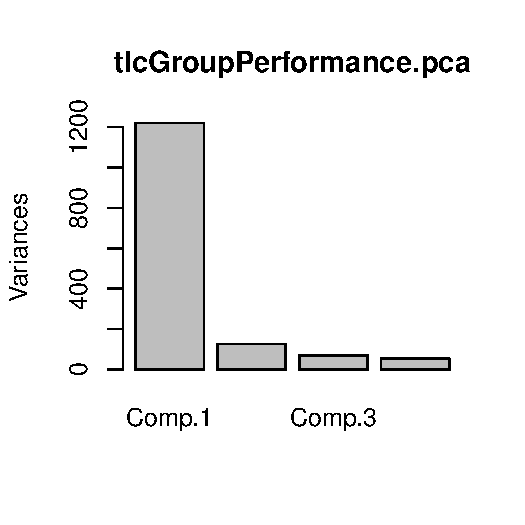
\includegraphics[width=\maxwidth]{figure/dataReductionGroupPerformance-1} 

}


\begin{kframe}

{\ttfamily\noindent\itshape\color{messagecolor}{\#\# \\\#\# Attaching package: 'psych'}}

{\ttfamily\noindent\itshape\color{messagecolor}{\#\# The following objects are masked from 'package:scales':\\\#\# \\\#\#\ \ \ \  alpha, rescale}}

{\ttfamily\noindent\itshape\color{messagecolor}{\#\# The following objects are masked from 'package:ggplot2':\\\#\# \\\#\#\ \ \ \  \%+\%, alpha}}\end{kframe}
\end{knitrout}



\begin{knitrout}
\definecolor{shadecolor}{rgb}{0.969, 0.969, 0.969}\color{fgcolor}\begin{kframe}


{\ttfamily\noindent\itshape\color{messagecolor}{\#\# Loading required package: Hmisc}}

{\ttfamily\noindent\color{warningcolor}{\#\# Warning: package 'Hmisc' was built under R version 3.3.2}}

{\ttfamily\noindent\itshape\color{messagecolor}{\#\# Loading required package: lattice}}

{\ttfamily\noindent\itshape\color{messagecolor}{\#\# Loading required package: survival}}

{\ttfamily\noindent\itshape\color{messagecolor}{\#\# Loading required package: Formula}}

{\ttfamily\noindent\itshape\color{messagecolor}{\#\# \\\#\# Attaching package: 'Hmisc'}}

{\ttfamily\noindent\itshape\color{messagecolor}{\#\# The following object is masked from 'package:psych':\\\#\# \\\#\#\ \ \ \  describe}}

{\ttfamily\noindent\itshape\color{messagecolor}{\#\# The following objects are masked from 'package:dplyr':\\\#\# \\\#\#\ \ \ \  combine, src, summarize}}

{\ttfamily\noindent\itshape\color{messagecolor}{\#\# The following objects are masked from 'package:xtable':\\\#\# \\\#\#\ \ \ \  label, label<-}}

{\ttfamily\noindent\itshape\color{messagecolor}{\#\# The following objects are masked from 'package:base':\\\#\# \\\#\#\ \ \ \  format.pval, round.POSIXt, trunc.POSIXt, units}}\end{kframe}
\end{knitrout}

Items concerning components of group performance in the invasion drill (defence, attack, support play, and on field communication) were subjected to EFA.  
Correlations between group component performance items was very high (all r's > 0.67), which suggested that one factor was appropriate (see Table ~\ref{tab:jointActionSuccessCorrTable}). 
The KMO index and Bartlett's test both suggested high sampling adequacy, (KMO =  0.83, \chi^2(6, N = 116) = 379.2793158, p = 0. One factor, labelled ``Joint Action Success'' was imposed on the data, which explained 77\% of the overall variance (SS Loading = 3.08). 
Guttmans \lambda = 0.92 and Cronbachs \alpha = 0.93 indicated that the data reduction was appropriate and reliable.


\myparagraph{Perceptions of Individual Component Performance}
\begin{knitrout}
\definecolor{shadecolor}{rgb}{0.969, 0.969, 0.969}\color{fgcolor}

{\centering 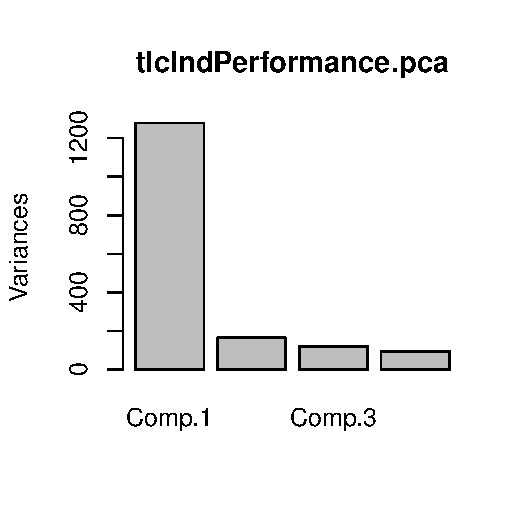
\includegraphics[width=\maxwidth]{figure/dataReductionIndPerformance-1} 

}



\end{knitrout}

Items concerning components of individual components of performance in the invasion drill (1-on-1 defence, passing technique, support play in attack, decision making in attack, and effectiveness in contact) were subjected to EFA.  The variable ``effectiveness in contact'' was removed from analysis as the invasion drill was predominantly a non-contact training drill, and so this item was not relevant to athletes' performance.  Correlations between individual component performance items was very high (all r's > 0.61), which suggested that one factor was appropriate (see Table ~\ref{tab:indComponentPerfCorrTable}). 
The KMO index and Bartlett's test both suggested high sampling adequacy, (KMO =  0.83, \chi^2(6, N = 116) = 280.6991709, p = 0. One factor, labelled ``Individual Performance Components'' was imposed on the data, which explained 69.1 \% of the overall variance (SS Loading = 2.77).  Guttmans \lambda = 0.87  and  Cronbachs \alpha = 0.9  indicated that the data reduction was appropriate and reliable.

\begin{knitrout}
\definecolor{shadecolor}{rgb}{0.969, 0.969, 0.969}\color{fgcolor}\begin{kframe}
\begin{alltt}
\hlcom{# be sure to import the variable subset data frame, not the correlation matrix}
\hlkwd{corstarsl}\hlstd{(tlcIndPerformance)}
\hlkwd{print}\hlstd{(}\hlkwd{xtable}\hlstd{(}\hlkwd{corstarsl}\hlstd{(tlcIndPerformance),} \hlkwc{type}\hlstd{=}\hlstr{"latex"}\hlstd{,}
                    \hlkwc{caption} \hlstd{=} \hlstr{"Correlations between components of individual performance"}\hlstd{,}
                    \hlkwc{label} \hlstd{=} \hlstr{"tab:indComponentPerfCorrTable"}\hlstd{),}
                    \hlkwc{file} \hlstd{=} \hlstr{"indComponengtPerfCorrTable.tex"}\hlstd{)}
\hlcom{# label = tab:indComponentPerformanceCorrTable}
\end{alltt}
\end{kframe}
\end{knitrout}


%Appendix
%% This is a follow-up EFA with individual and group performance in one matrix.
%<<dataReductionPerformanceAll, eval=TRUE, echo=FALSE>>=
%min(competenceMatrix)

%# 2. jointActionSuccess and individualComponentPerformance:
%#PerformanceComponentsTogether:
%tlcPerformance <- subset(tlc, select = c(groupDefensiveLine, groupAttackingLine,        groupSupportPlay, groupOnfieldCommunication, indDefense, passingTechnique, supportPlay, decisionMaking, effectivenessInContact))

%tlcPerformance.fa <- factanal(~ groupDefensiveLine + groupAttackingLine + groupSupportPlay + groupOnfieldCommunication +
                              %indDefense + passingTechnique + supportPlay + %decisionMaking + effectivenessInContact, 2,
                                 %data = tlc, rotation = "promax", na.action = na.exclude, %scores = "regression")
%tlcPerformance.fa

%tlcPerformanceMatrix <- cor(tlcPerformance, use = "complete")
%KMO(tlcPerformanceMatrix)
%library(psych)
%cortest.bartlett(tlcPerformanceMatrix, n = 116) # what is the sample size here?
%psych::alpha(tlcPerformanceMatrix)
%@



\myparagraph{Feelings of team click within training group}

\begin{knitrout}
\definecolor{shadecolor}{rgb}{0.969, 0.969, 0.969}\color{fgcolor}

{\centering 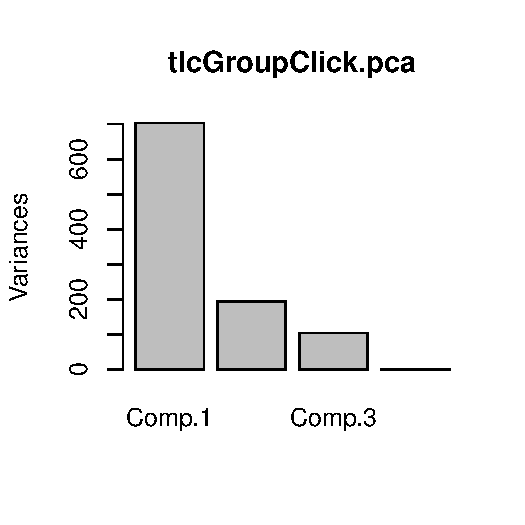
\includegraphics[width=\maxwidth]{figure/dataReductionGroupClick-1} 

}



\end{knitrout}


\begin{knitrout}
\definecolor{shadecolor}{rgb}{0.969, 0.969, 0.969}\color{fgcolor}

{\centering 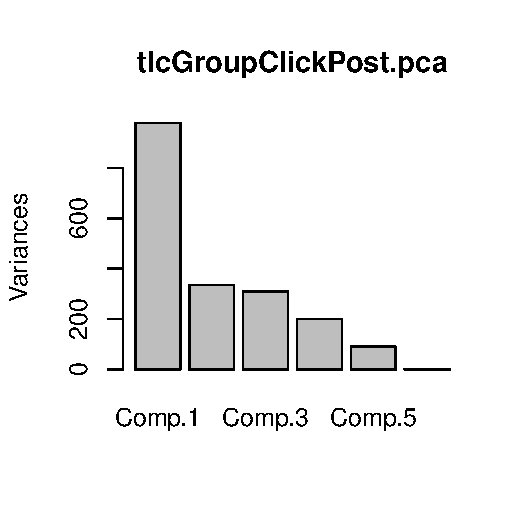
\includegraphics[width=\maxwidth]{figure/dataReductionGroupClickPost-1} 

}



\end{knitrout}


Items relating to training group team click (unspoken understanding, general atmosphere, click pictorial, and ability extended by the group) were subjected to EFA.    Correlations between the remaining were very high (all r's > 0.29), which suggested that one factor was appropriate (see Table ee Table ~\ref{tab:groupClickCorrTable}). The KMO index and Bartlett's test both suggested high sampling adequacy, (KMO =  0.72, \chi^2(6, N = 116) = 127.8567081, p = 0).  
One factor, labelled ``Group Click'' was imposed on the data, which explained 47.7\% of the overall variance (SS Loading = 1.91). Guttmans \lambda = 0.73 and Cronbachs \alpha = 0.77 indicated that the data reduction was appropriate and reliable.


In addition to the four variables common to both pre- and post-experiment surveys, athletes were also asked in the post-experiment survey about their own reliability and the reliability of other athletes to perform their role on the field specifically. These two variables, ``Reliability For Others'' and ``Reliability Of Others'' were included in an EFA involving only the post-experiment measures.

The variable ``reliability for others'' was removed from the matrix because it did not significantly correlate with other variables (all r's <= .16).




\begin{knitrout}
\definecolor{shadecolor}{rgb}{0.969, 0.969, 0.969}\color{fgcolor}\begin{kframe}
\begin{alltt}
\hlcom{# be sure to import the variable subset data frame, not the correlation matrix}
\hlkwd{corstarsl}\hlstd{(tlcGroupClickPost)}
\hlkwd{print}\hlstd{(}\hlkwd{xtable}\hlstd{(}\hlkwd{corstarsl}\hlstd{(tlcGroupClick),} \hlkwc{type}\hlstd{=} \hlstr{"latex"}\hlstd{,}
                    \hlkwc{caption} \hlstd{=} \hlstr{"Correlations between variables of group click"}\hlstd{,}
                    \hlkwc{label} \hlstd{=} \hlstr{"tab:groupClickCorrTable"}\hlstd{),}
                    \hlkwc{file} \hlstd{=} \hlstr{"groupClickCorrTable.tex"}\hlstd{)}
\hlcom{# label = tab:groupClickCorrTable}
\end{alltt}
\end{kframe}
\end{knitrout}





\myparagraph{Feelings of Social Bonding to the training group}
\begin{knitrout}
\definecolor{shadecolor}{rgb}{0.969, 0.969, 0.969}\color{fgcolor}

{\centering 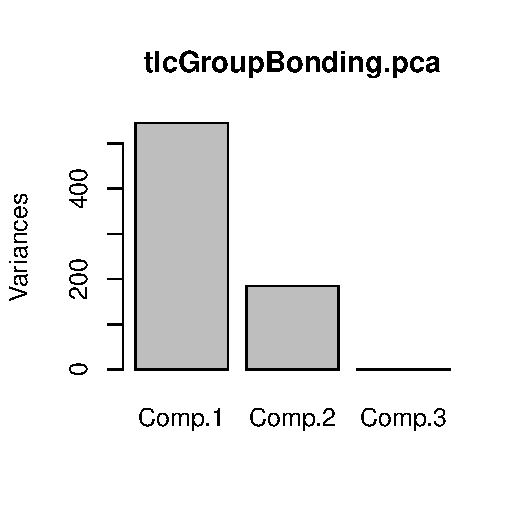
\includegraphics[width=\maxwidth]{figure/dataReductionGroupBonding-1} 

}



\end{knitrout}



\begin{knitrout}
\definecolor{shadecolor}{rgb}{0.969, 0.969, 0.969}\color{fgcolor}\begin{kframe}
\begin{alltt}
\hlcom{# be sure to import the variable subset data frame, not the correlation matrix}
\hlkwd{corstarsl}\hlstd{(tlcGroupBonding)}
\hlkwd{print}\hlstd{(}\hlkwd{xtable}\hlstd{(}\hlkwd{corstarsl}\hlstd{(tlcGroupBonding),} \hlkwc{type}\hlstd{=}\hlstr{"latex"}\hlstd{,}
                    \hlkwc{caption} \hlstd{=} \hlstr{"Correlations between group bonding variables"}\hlstd{,}
                    \hlkwc{label} \hlstd{=} \hlstr{"tab:groupBondingCorrTable"}\hlstd{),}
                    \hlkwc{file} \hlstd{=} \hlstr{"groupBondingCorrTable.tex"}\hlstd{)}
\hlcom{# label = tab:groupBondingCorrTable}
\end{alltt}
\end{kframe}
\end{knitrout}

Items concerning bonding to the training group (emotional support, shared goal, fusion pictorial) were subjected to EFA.  Correlations between items were high (all r's > 0.37), which suggested that one factor would be appropriate (see Table ee Table ~\ref{tab:groupBondingCorrTable}). The KMO index and Bartlett's test both suggested high sampling adequacy, (KMO =  0.65, \chi^2(3, N = 116) = 54.2305691, p = 0).
One factor, labelled ``Group Social Bonding'' was imposed on the data, which explained 42\% of the overall variance (SS Loading = 1.26). Guttmans \lambda = 0.59 and Cronbachs \alpha = 0.68 indicated that the data reduction was appropriate and reliable.



%team click
% "teamClickPictorial_1"  # TEAM CLICK post not measured
% [94] "reliabilityForOthers_1" # TEAM RELIABILITY - i don't ask about the team as a whole post-experiment...
% [95] "reliabilityOfOthers_1"
\subsubsection{Social Bonding to the team}



\begin{knitrout}
\definecolor{shadecolor}{rgb}{0.969, 0.969, 0.969}\color{fgcolor}\begin{kframe}
\begin{alltt}
\hlcom{# be sure to import the variable subset data frame, not the correlation matrix}
\hlkwd{corstarsl}\hlstd{(tlcTeamBonding)}
\hlkwd{print}\hlstd{(}\hlkwd{xtable}\hlstd{(}\hlkwd{corstarsl}\hlstd{(tlcTeamBonding),} \hlkwc{type}\hlstd{=}\hlstr{"latex"}\hlstd{,}
                    \hlkwc{caption} \hlstd{=} \hlstr{"Correlations between team bonding variables"}\hlstd{,}
                    \hlkwc{label} \hlstd{=} \hlstr{"tab:teamBondingCorrTable"}\hlstd{),}
                    \hlkwc{file} \hlstd{=} \hlstr{"teamBondingCorrTable.tex"}\hlstd{)}
\hlcom{# label = tab:teamBondingCorrTable}
\end{alltt}
\end{kframe}
\end{knitrout}



Items concerning bonding to the team (emotional support, shared goal, fusion pictorial, fusion verbal, and group identification) were subjected to EFA.  Correlations between items were all reasonably high (all r's > 0.18), which suggested that one factor would be appropriate (see Table ee Table ~\ref{tab:teamBondingCorrTable}). 
The KMO index and Bartlett's test both suggested high sampling adequacy, (KMO =  0.7, \chi^2(10, N = 116) = 172.5861663, p = 0).
One factor, labelled ``Team Social Bonding'' was imposed on the data, which explained 39.2 \% of the overall variance (SS Loading = 1.96). Guttmans \lambda = 0.77 and Cronbachs \alpha = 0.76 indicated that the data reduction was appropriate and reliable.



\myparagraph{Arousal}




\begin{knitrout}
\definecolor{shadecolor}{rgb}{0.969, 0.969, 0.969}\color{fgcolor}\begin{kframe}
\begin{alltt}
\hlcom{# be sure to import the variable subset data frame, not the correlation matrix}
\hlkwd{corstarsl}\hlstd{(tlcArousal)}
\hlkwd{print}\hlstd{(}\hlkwd{xtable}\hlstd{(}\hlkwd{corstarsl}\hlstd{(tlcArousal),} \hlkwc{type}\hlstd{=}\hlstr{"latex"}\hlstd{,}
                    \hlkwc{caption} \hlstd{=} \hlstr{"Correlations between variables measuring arousal"}\hlstd{,}
                    \hlkwc{label} \hlstd{=} \hlstr{"tab:arousalCorrTable"}\hlstd{),}
                    \hlkwc{file} \hlstd{=} \hlstr{"arousalCorrTable.tex"}\hlstd{)}
\hlcom{# label = tab:arousalCorrTable}
\end{alltt}
\end{kframe}
\end{knitrout}

Items associated with team discipline (punctuality, observing bed times and curfews, attendance at meals, general team conduct), measured at baseline and after the experiment, were subjected to EFA.  
Correlations between items were all reasonably high (all r's > 0.42), which suggested that one factor would be appropriate (see Table ee Table ~\ref{tab:arousalCorrTable}). The KMO index and Bartlett's test both suggested high sampling adequacy, (KMO =  0.64, \chi^2(3, N = 116) = 116.1210816, p = 0).
One factor, labelled ``Team Discipline'' was imposed on the data, which explained 58.7\% of the overall variance (SS Loading = 1.76).  Guttmans \lambda = 0.74  and  Cronbachs \alpha = 0.78  indicated that the data reduction was appropriate and reliable.



\subsubsection{Athlete Technical Competence (objective and subjective measures)}



\begin{knitrout}
\definecolor{shadecolor}{rgb}{0.969, 0.969, 0.969}\color{fgcolor}\begin{kframe}
\begin{alltt}
\hlcom{# be sure to import the variable subset data frame, not the correlation matrix}
\hlkwd{corstarsl}\hlstd{(tlcTechnicalCompetence)}
\hlkwd{print}\hlstd{(}\hlkwd{xtable}\hlstd{(}\hlkwd{corstarsl}\hlstd{(tlcTechnicalCompetence),} \hlkwc{type}\hlstd{=}\hlstr{"latex"}\hlstd{,}
                    \hlkwc{caption} \hlstd{=} \hlstr{"Correlations between measures of technical competence"}\hlstd{,}
                    \hlkwc{label} \hlstd{=} \hlstr{"tab:technicalCompetenceCorrTable"}\hlstd{),}
                    \hlkwc{file} \hlstd{=} \hlstr{"technicalCompetenceCorrTable.tex"}\hlstd{)}
\hlcom{# label = tab:technicalCompetenceCorrTable}
\end{alltt}
\end{kframe}
\end{knitrout}



All eight items relevant to technical competence were analysed in a correlation matrix to assess relatedness (see Table ~\ref{tab:technicalCompetenceCorrTable}). All measures of objective competence were highly correlated all r's >= NA),  and among measures of subjective competence (all items except for the team competence measure correlated at $> NA)$) suggested that the data could be explained by two underlying factors. Team Ability Chinese Provinces was dropped from analysis due to low correlation with other competence variables, possibly because the item did not ask about an individual athlete’s competence (it referred instead to an athlete’s opinion of the competence of the team of which they were a member).

An EFA of technical competence variables revealed that items of interest loaded on two factors. Measures of objective competence (Years Team, Training Age, Team Status, Athlete Status) loaded on the first factor, which was labelled ``Objective Competence'' because the measures were all objective markers of an athlete's competence.
Objective Competence explained 41\% of the total variance (2.87). The remaining measures of subjective competence (Ability Teammates, Ability Chinese Pros, Ability International Pros) loaded on the remaining factor.  The second factor was labelled ``Subjective Competence'', due to the fact that all measures were the product of athlete self-report.  Subjective competence explained 41\% of the variance (1.62).
$Guttmans \lambda = 0.86$ and $Cronbachs \alpha = 0.79$ indicated that the data reduction was appropriate and reliable.








\subsubsection{Team Discipline}





\begin{knitrout}
\definecolor{shadecolor}{rgb}{0.969, 0.969, 0.969}\color{fgcolor}\begin{kframe}
\begin{alltt}
\hlcom{# be sure to import the variable subset data frame, not the correlation matrix}
\hlkwd{corstarsl}\hlstd{(tlcTeamDiscipline)}
\hlkwd{print}\hlstd{(}\hlkwd{xtable}\hlstd{(}\hlkwd{corstarsl}\hlstd{(tlcTeamDiscipline),} \hlkwc{type}\hlstd{=}\hlstr{"latex"}\hlstd{,}
                    \hlkwc{caption} \hlstd{=} \hlstr{"Correlations between variables measuring team discipline"}\hlstd{,}
                    \hlkwc{label} \hlstd{=} \hlstr{"tab:teamDisciplineCorrTable"}\hlstd{),}
                    \hlkwc{file} \hlstd{=} \hlstr{"teamDisciplineCorrTable.tex"}\hlstd{)}
\hlcom{# label = tab:teamDisciplineCorrTable}
\end{alltt}
\end{kframe}
\end{knitrout}

Items concerning team discipline (attendance at meals, team curfew, general team conduct, punctuality to team engagements), measured at baseline and after the experiment, were subjected to EFA.  Correlations between items were all reasonably high (all r's > 0.63), which suggested that one factor would be appropriate (see Table ee Table ~\ref{tab:teamDisciplineCorrTable}). 
The KMO index and Bartlett's test both suggested high sampling adequacy, (KMO =  0.78, \chi^2(6, N = 116) = 362.748819, p = 0).  
One factor, labelled ``Team Discipline'' was imposed on the data, which explained 73.9 \% of the overall variance (SS Loading = 2.96).  Guttmans \lambda = 0.91  and  Cronbachs \alpha = 0.92  indicated that the data reduction was appropriate and reliable.


% \myparagraph{Fatigue} - fatigue is measured pre and post experiment, but mental and prpe are measured only post-experiment, so no need for EFA






\subsection{Manipulation Checks}
The effectiveness of the experimental manipulation was assesed based on a comparison of athletes responses to three survey items immediately following the high or low difficulty prime and immediately before the training drill.  Athletes were asked about their confidence in their individual and training group's ability to handle the technical challenges of the training drill.  Due to the fact that athletes had been primed to expect either a difficult or simple training drill, it was expected that athletes in the high difficulty condition would be less confident about their own and their group's ability to meet the technical challenges of the training session. In addition to self-reported confidence, it was also predicted that athlete self-reports of arousal, measured measured at the same time as the previous questions regarding confidence, would also vary according to condition.  It was predicted that that athletes in the high difficulty condition would be more aroused than athtletes in the low difficulty condition.  Meaningful variation in these variables could be used to check that the experimental manipulation was successful.








%%% group confidence in technical challenges:
\begin{knitrout}
\definecolor{shadecolor}{rgb}{0.969, 0.969, 0.969}\color{fgcolor}\begin{kframe}
\begin{alltt}
\hlkwd{boxplot}\hlstd{(groupConfidentTechnicalChallenges_2} \hlopt{~} \hlstd{condition,}
                                        \hlkwc{varwidth} \hlstd{=} \hlnum{TRUE}\hlstd{,}
                                        \hlkwc{width} \hlstd{=} \hlkwd{c}\hlstd{(}\hlnum{.5}\hlstd{,}\hlnum{.5}\hlstd{),}
                                        \hlkwc{notch} \hlstd{= F,}
                                        \hlkwc{main} \hlstd{=} \hlstr{"Confidence in group to \textbackslash{}n meet technical challenges"}\hlstd{,}
                                        \hlkwc{xlab} \hlstd{=} \hlstr{"Condition"}\hlstd{,}
                                        \hlkwc{ylab} \hlstd{=} \hlstr{"Confidence"}\hlstd{,}
                                        \hlkwc{data} \hlstd{= twc)}
\end{alltt}
\end{kframe}\begin{figure}

{\centering 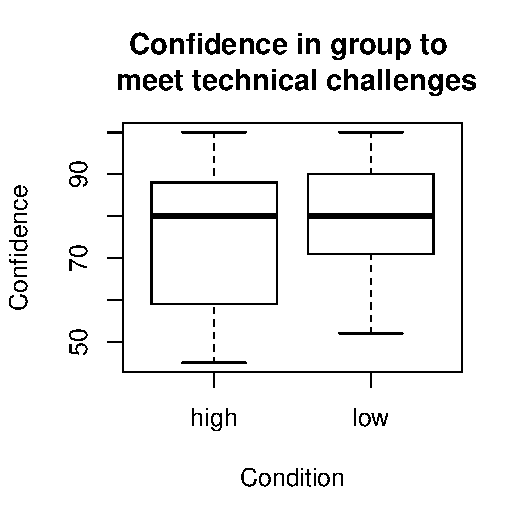
\includegraphics[width=\maxwidth]{figure/groupConfChallengesBoxplot-1} 

}

\end{figure}


\end{knitrout}

\begin{knitrout}
\definecolor{shadecolor}{rgb}{0.969, 0.969, 0.969}\color{fgcolor}\begin{kframe}
\begin{alltt}
\hlkwd{hist}\hlstd{(high}\hlopt{$}\hlstd{groupConfidentTechnicalChallenges_2,}
                                        \hlkwc{main} \hlstd{=}  \hlstr{"Histogram of confidence in group to \textbackslash{}n meet technical challenges (high difficulty)"}\hlstd{,}
                                        \hlkwc{xlab} \hlstd{=} \hlstr{"Confidence"}\hlstd{,}
                                        \hlkwc{xlim} \hlstd{=} \hlkwd{c}\hlstd{(}\hlnum{0}\hlstd{,} \hlnum{100}\hlstd{))}
\end{alltt}
\end{kframe}\begin{figure}

{\centering 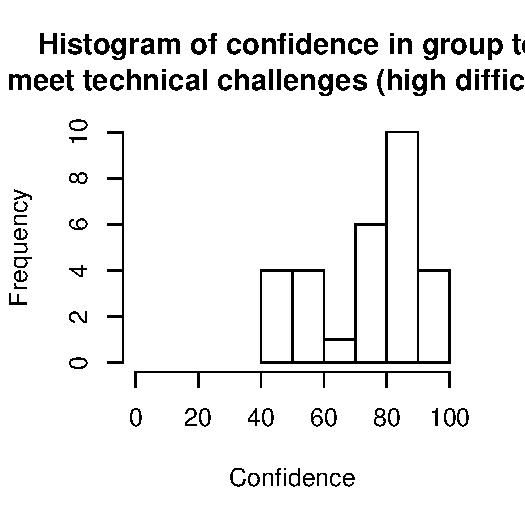
\includegraphics[width=\maxwidth]{figure/histHighGroupConfidence-1} 

}

\end{figure}


\end{knitrout}

\begin{knitrout}
\definecolor{shadecolor}{rgb}{0.969, 0.969, 0.969}\color{fgcolor}\begin{kframe}
\begin{alltt}
\hlkwd{hist}\hlstd{(low}\hlopt{$}\hlstd{groupConfidentTechnicalChallenges_2,}
                                        \hlkwc{main} \hlstd{=}  \hlstr{"Histogram of confidence in group to \textbackslash{}n meet technical challenges (low difficulty)"}\hlstd{,}
                                        \hlkwc{xlab} \hlstd{=} \hlstr{"Confidence"}\hlstd{,}
                                        \hlkwc{xlim} \hlstd{=} \hlkwd{c}\hlstd{(}\hlnum{0}\hlstd{,} \hlnum{100}\hlstd{))}
\end{alltt}
\end{kframe}\begin{figure}

{\centering 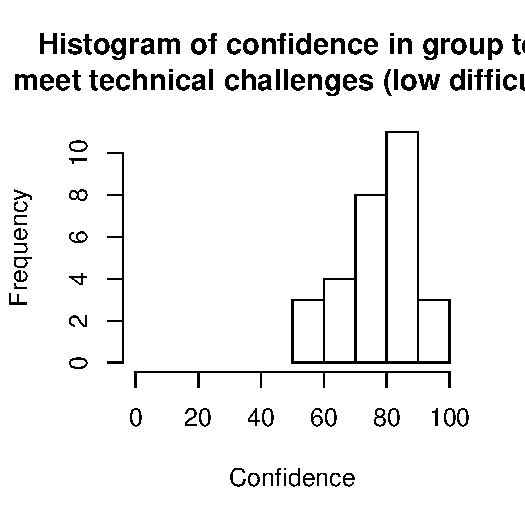
\includegraphics[width=\maxwidth]{figure/histLowGroupConfidence-1} 

}

\end{figure}


\end{knitrout}

\begin{knitrout}
\definecolor{shadecolor}{rgb}{0.969, 0.969, 0.969}\color{fgcolor}\begin{kframe}


{\ttfamily\noindent\color{warningcolor}{\#\# Warning: package 'car' was built under R version 3.3.2}}

{\ttfamily\noindent\itshape\color{messagecolor}{\#\# \\\#\# Attaching package: 'car'}}

{\ttfamily\noindent\itshape\color{messagecolor}{\#\# The following object is masked from 'package:psych':\\\#\# \\\#\#\ \ \ \  logit}}

{\ttfamily\noindent\itshape\color{messagecolor}{\#\# The following object is masked from 'package:dplyr':\\\#\# \\\#\#\ \ \ \  recode}}\end{kframe}
\end{knitrout}



\begin{knitrout}
\definecolor{shadecolor}{rgb}{0.969, 0.969, 0.969}\color{fgcolor}\begin{kframe}
\begin{alltt}
\hlstd{indConfConditionBoxPlot} \hlkwb{<-} \hlkwd{boxplot}\hlstd{(indConfidenceChallenges_2} \hlopt{~} \hlstd{condition,}
                                        \hlkwc{varwidth} \hlstd{=} \hlnum{TRUE}\hlstd{,}
                                        \hlkwc{width} \hlstd{=} \hlkwd{c}\hlstd{(}\hlnum{.5}\hlstd{,}\hlnum{.5}\hlstd{),}
                                        \hlkwc{notch} \hlstd{= F,}
                                        \hlkwc{main} \hlstd{=} \hlstr{"Confidence in individual ability \textbackslash{}n to meet technical challenges"}\hlstd{,}
                                        \hlkwc{xlab} \hlstd{=} \hlstr{"Condition"}\hlstd{,}
                                        \hlkwc{ylab} \hlstd{=} \hlstr{"Confidence"}\hlstd{,}
                                        \hlkwc{data} \hlstd{= twc)}
\end{alltt}
\end{kframe}\begin{figure}

{\centering 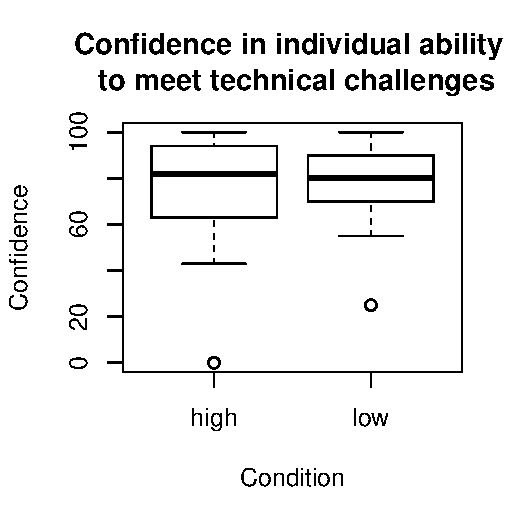
\includegraphics[width=\maxwidth]{figure/indConfChallengesBoxplot-1} 

}

\end{figure}


\end{knitrout}

\begin{knitrout}
\definecolor{shadecolor}{rgb}{0.969, 0.969, 0.969}\color{fgcolor}\begin{kframe}
\begin{alltt}
\hlstd{histHighIndConfidence} \hlkwb{<-} \hlkwd{hist}\hlstd{(high}\hlopt{$}\hlstd{indConfidenceChallenges_2,}
                                        \hlkwc{main} \hlstd{=}  \hlstr{"Histogram of confidence in individual \textbackslash{}n ability to meet technical challenges \textbackslash{}n (high difficulty)"}\hlstd{,}
                                        \hlkwc{xlab} \hlstd{=} \hlstr{"Confidence"}\hlstd{,}
                                        \hlkwc{xlim} \hlstd{=} \hlkwd{c}\hlstd{(}\hlnum{0}\hlstd{,} \hlnum{100}\hlstd{),}
                                        \hlkwc{ylim} \hlstd{=} \hlkwd{c}\hlstd{(}\hlnum{0}\hlstd{,} \hlnum{20}\hlstd{))}
\end{alltt}
\end{kframe}\begin{figure}

{\centering 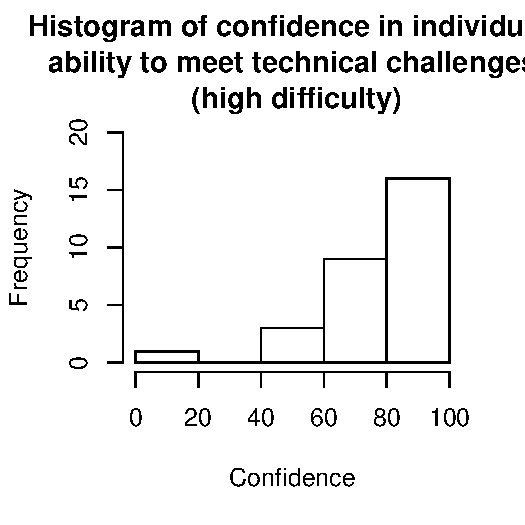
\includegraphics[width=\maxwidth]{figure/histHighIndConfidence-1} 

}

\end{figure}


\end{knitrout}

\begin{knitrout}
\definecolor{shadecolor}{rgb}{0.969, 0.969, 0.969}\color{fgcolor}\begin{kframe}
\begin{alltt}
\hlstd{histLowIndConfidence} \hlkwb{<-} \hlkwd{hist}\hlstd{(low}\hlopt{$}\hlstd{indConfidenceChallenges_2,} \hlkwc{main} \hlstd{=}
                                        \hlstr{"Histogram of condifence in in individual \textbackslash{}n ability to meet technical challenges \textbackslash{}n (low difficulty)"}\hlstd{,}
                                        \hlkwc{xlab} \hlstd{=} \hlstr{"Confidence"}\hlstd{,}
                                        \hlkwc{xlim} \hlstd{=} \hlkwd{c}\hlstd{(}\hlnum{0}\hlstd{,} \hlnum{100}\hlstd{),}
                                        \hlkwc{ylim} \hlstd{=} \hlkwd{c}\hlstd{(}\hlnum{0}\hlstd{,} \hlnum{20}\hlstd{))}
\end{alltt}
\end{kframe}\begin{figure}

{\centering 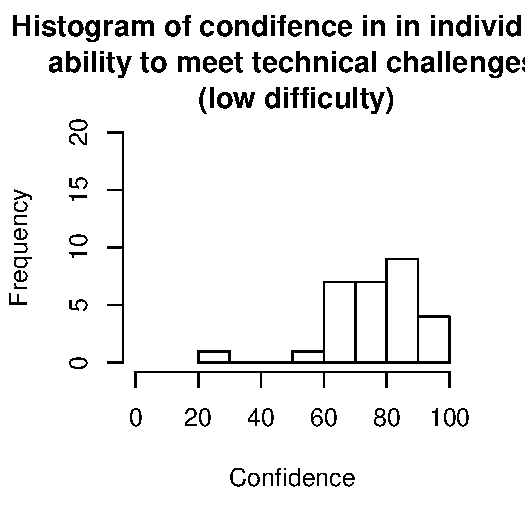
\includegraphics[width=\maxwidth]{figure/histLowIndConfidence-1} 

}

\end{figure}

\begin{kframe}\begin{alltt}
\hlcom{# t.test(high$indConfidenceChallenges_2, low$indConfidenceChallenges_2)}
\end{alltt}
\end{kframe}
\end{knitrout}


\begin{knitrout}
\definecolor{shadecolor}{rgb}{0.969, 0.969, 0.969}\color{fgcolor}\begin{kframe}


{\ttfamily\noindent\bfseries\color{errorcolor}{\#\# Error in contrib.url(repos, "{}source"{}): trying to use CRAN without setting a mirror}}

{\ttfamily\noindent\bfseries\color{errorcolor}{\#\# Error in cohens\_d.htest(indPerfBartlett, format = "{}latex"{}): ttest must be a call to either `t\_test` or `t.test`}}

{\ttfamily\noindent\bfseries\color{errorcolor}{\#\# Error in apa(indPerfBartlett): Unkown type passed to 'x'}}\end{kframe}
\end{knitrout}

%(t_test(groupConfidenceCondition.ttest)) 
 %(t_test(indConfidenceCondition.ttest)) 
Results of manipulation checks indicate that there were no overall condition-wise differences in athlete confidence in group or individual ability to meet the technical challenges of the drill (see Table ~\ref{tab:manipulationCheckTable} and Figures ~\ref{fig:groupConfChallengesBoxplot} and ~\ref{fig:indConfChallengesBoxplot}).
Although the central tendency of these variables was not significantly different, the box plots (Figures ~\ref{fig:groupConfChallengesBoxplot}) and histograms of both group and individual confidence variables by condition show that the variance in responses in the high difficulty condition appears to be larger than the low difficulty condition (see Figures ~\ref{fig:histHighGroupConfidence}\nobreakdash~\ref{fig:histLowIndConfidence}).
A Bartlett's test of homogeneity of variance revealed that there was no meaningful difference in variance of confidence in group ability (2.39556133520555, 1, 0.12168006558935, groupConfidentTechnicalChallenges_2 by condition, Bartlett test of homogeneity of variances). The same test applied to athlete confidence in individual ability according to condition did, however, reveal a significant difference, 2.17299490056626, c(28, 28), 0.0443622290888093, c(1.02022166316948, 4.62831461862671), 2.17299490056626, 1, two.sided, F test to compare two variances, high$indConfidenceChallenges_2 and low$indConfidenceChallenges_2.



\begin{knitrout}
\definecolor{shadecolor}{rgb}{0.969, 0.969, 0.969}\color{fgcolor}\begin{kframe}
\begin{alltt}
\hlstd{arousalFactorPreBoxPlot} \hlkwb{<-} \hlkwd{boxplot}\hlstd{(arousalFactorPre} \hlopt{~} \hlstd{condition,}
                                        \hlkwc{varwidth} \hlstd{=} \hlnum{TRUE}\hlstd{,}
                                        \hlkwc{width} \hlstd{=} \hlkwd{c}\hlstd{(}\hlnum{.5}\hlstd{,}\hlnum{.5}\hlstd{),}
                                        \hlkwc{notch} \hlstd{= F,}
                                        \hlkwc{main} \hlstd{=} \hlstr{"Athlete arousal prior to experiment"}\hlstd{,}
                                        \hlkwc{xlab} \hlstd{=} \hlstr{"Condition"}\hlstd{,}
                                        \hlkwc{ylab} \hlstd{=} \hlstr{"Arousal"}\hlstd{,}
                                        \hlkwc{data} \hlstd{= twc)}
\end{alltt}
\end{kframe}\begin{figure}

{\centering 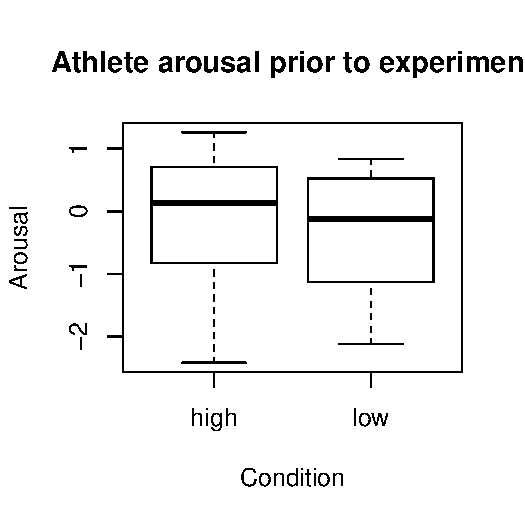
\includegraphics[width=\maxwidth]{figure/arousalFactorPreBoxPlot-1} 

}

\end{figure}


\end{knitrout}


\begin{knitrout}
\definecolor{shadecolor}{rgb}{0.969, 0.969, 0.969}\color{fgcolor}\begin{kframe}
\begin{alltt}
\hlstd{histArousalFactorPreHigh} \hlkwb{<-} \hlkwd{hist}\hlstd{(high}\hlopt{$}\hlstd{arousalFactorPre,}
                                        \hlkwc{main} \hlstd{=}  \hlstr{"Histogram of athlete arousal \textbackslash{}n prior to experiment (high difficulty)"}\hlstd{,}
                                        \hlkwc{xlab} \hlstd{=} \hlstr{"Arousal"}\hlstd{,}
                                        \hlkwc{xlim} \hlstd{=} \hlkwd{c}\hlstd{(}\hlopt{-}\hlnum{3}\hlstd{,} \hlnum{2}\hlstd{),}
                                        \hlkwc{ylim} \hlstd{=} \hlkwd{c}\hlstd{(}\hlnum{0}\hlstd{,}\hlnum{10}\hlstd{))}
\end{alltt}
\end{kframe}\begin{figure}

{\centering 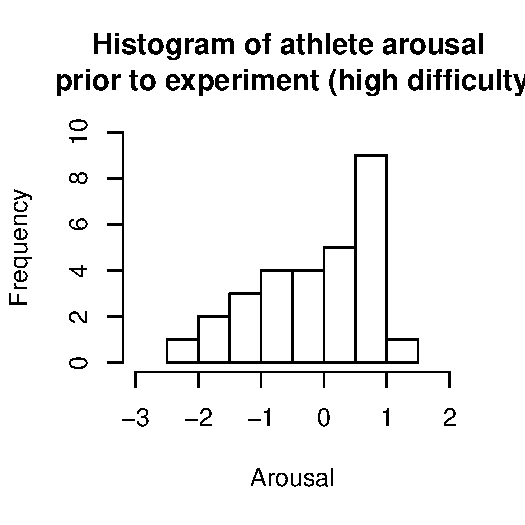
\includegraphics[width=\maxwidth]{figure/histArousalFactorPreHigh-1} 

}

\end{figure}


\end{knitrout}

\begin{knitrout}
\definecolor{shadecolor}{rgb}{0.969, 0.969, 0.969}\color{fgcolor}\begin{kframe}
\begin{alltt}
\hlkwd{hist}\hlstd{(low}\hlopt{$}\hlstd{arousalFactorPre,} \hlkwc{main} \hlstd{=}  \hlstr{"Histogram of athlete arousal \textbackslash{}n prior to experiment
                              (low difficulty)"}\hlstd{,}
                              \hlkwc{xlab} \hlstd{=} \hlstr{"Arousal"}\hlstd{,}
                              \hlkwc{xlim} \hlstd{=} \hlkwd{c}\hlstd{(}\hlopt{-}\hlnum{3}\hlstd{,} \hlnum{2}\hlstd{),}
                              \hlkwc{ylim} \hlstd{=} \hlkwd{c}\hlstd{(}\hlnum{0}\hlstd{,}\hlnum{10}\hlstd{))}
\end{alltt}
\end{kframe}\begin{figure}

{\centering 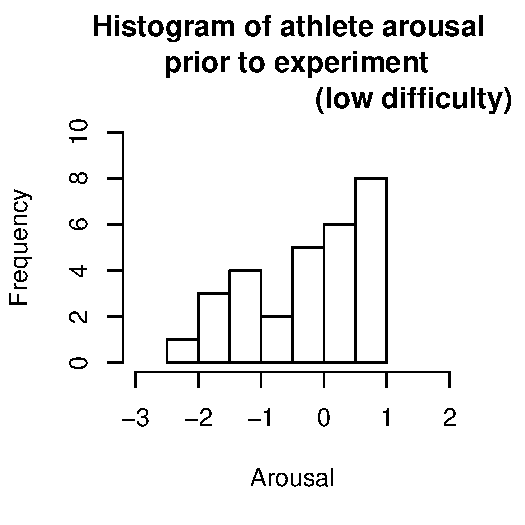
\includegraphics[width=\maxwidth]{figure/histArousalFactorPreLow-1} 

}

\end{figure}


\end{knitrout}



%t_apa(arousalCondition.ttest)
An analysis of arousal by condition also failed to reveal meaningful variation by condition, (see Table ~\ref{tab:manipulationCheckTable} and Figure ~\ref{fig:arousalFactorPreBoxPlot}). Judging by the boxplot and histogram of each condition (see Figures ~\ref{fig:histArousalFactorPreHigh} and ~\ref{fig:histArousalFactorPreLow} variance of arousal in the high difficulty condition did appear to be higher than the low difficulty condition, however a Bartlett's test for homogeneity of variance revealed that the difference was not significant, 0.46014520291942, 1, 0.497556120225506, arousalFactorPre by condition, Bartlett test of homogeneity of variances.

These results suggested that the experimental prime was not successful in modulating athlete self-reported confidence in individuala and group ability to meet the technical challenges associated with the training drill. There was also no evidence that self-reported arousal differed significantly according to condition.  It was still possible, however, that the experimental primes influenced dimensions of athlete behaviour dimensions inaccessible through self-report.


\subsection{Results by condition}
Predictions of this study were first tested according to condition. It was predicted that the high difficulty prime would generate closer attention to the details of joint action between participants, and more positive violation of expectations around group performance.



% latex table generated in R 3.3.0 by xtable 1.8-2 package
% Mon Oct  9 11:36:28 2017
\begin{table}[ht]
\centering
\begin{tabular}{rllll}
  \hline
 & high & low & p & test \\ 
  \hline
n &    29 &    29 &  &  \\ 
  JointActionSuccess (mean (sd)) & -0.40 (1.22) & -0.16 (0.74) &  0.373 &  \\ 
  IndividualComponentPerformance (mean (sd)) & -0.02 (1.06) & -0.10 (0.90) &  0.765 &  \\ 
  GroupPerformanceVsExpectations (mean (sd)) & 66.50 (20.64) & 66.83 (18.32) &  0.950 &  \\ 
  IndividualPerformanceVsExpectations (mean (sd)) & 64.79 (16.83) & 58.31 (17.71) &  0.163 &  \\ 
   \hline
\end{tabular}
\caption{Athlete perceptions of performance 
 post-experiment} 
\label{tab:performanceConditionPost}
\end{table}







%% jointACtionSuccess & indPerformance:
\begin{knitrout}
\definecolor{shadecolor}{rgb}{0.969, 0.969, 0.969}\color{fgcolor}\begin{kframe}
\begin{alltt}
\hlstd{groupJointActionSuccessBoxPlot} \hlkwb{<-} \hlkwd{boxplot}\hlstd{(jointActionSuccessPost} \hlopt{~} \hlstd{condition,}
                                        \hlkwc{varwidth} \hlstd{=} \hlnum{TRUE}\hlstd{,}
                                        \hlkwc{width} \hlstd{=} \hlkwd{c}\hlstd{(}\hlnum{.5}\hlstd{,}\hlnum{.5}\hlstd{),}
                                        \hlkwc{notch} \hlstd{= F,}
                                        \hlkwc{main} \hlstd{=} \hlstr{"Athlete post-experiment perceptions of \textbackslash{}n joint action success by condition \textbackslash{}n"}\hlstd{,}
                                        \hlkwc{xlab} \hlstd{=} \hlstr{"Condition"}\hlstd{,}
                                        \hlkwc{ylab} \hlstd{=} \hlstr{"Joint Action Success"}\hlstd{,}
                                        \hlkwc{data} \hlstd{= twc)}
\end{alltt}
\end{kframe}\begin{figure}

{\centering 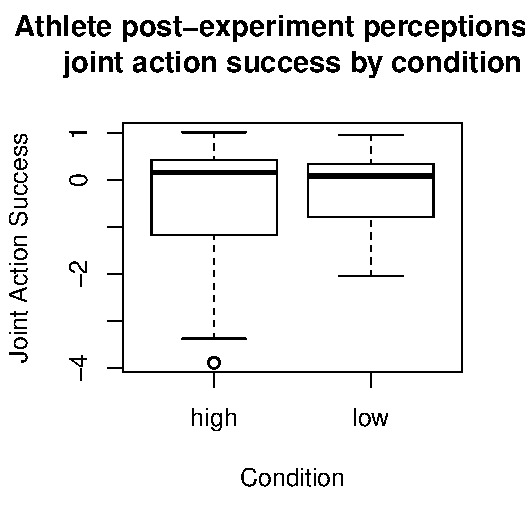
\includegraphics[width=\maxwidth]{figure/groupJointActionSuccessPostBoxPlot-1} 

}

\end{figure}


\end{knitrout}

\begin{knitrout}
\definecolor{shadecolor}{rgb}{0.969, 0.969, 0.969}\color{fgcolor}\begin{kframe}
\begin{alltt}
\hlstd{indComponentPerformancePostBoxPlot} \hlkwb{<-} \hlkwd{boxplot}\hlstd{(indPerformancePost} \hlopt{~} \hlstd{condition,}
                                        \hlkwc{varwidth} \hlstd{=} \hlnum{TRUE}\hlstd{,}
                                        \hlkwc{width} \hlstd{=} \hlkwd{c}\hlstd{(}\hlnum{.5}\hlstd{,}\hlnum{.5}\hlstd{),}
                                        \hlkwc{notch} \hlstd{= F,}
                                        \hlkwc{main} \hlstd{=} \hlstr{"Athlete post-experiment perceptions of \textbackslash{}n individual performance by condition \textbackslash{}n"}\hlstd{,}
                                        \hlkwc{xlab} \hlstd{=} \hlstr{"Condition"}\hlstd{,}
                                        \hlkwc{ylab} \hlstd{=} \hlstr{"Individual Performance"}\hlstd{,}
                                        \hlkwc{data} \hlstd{= twc)}
\end{alltt}
\end{kframe}\begin{figure}

{\centering 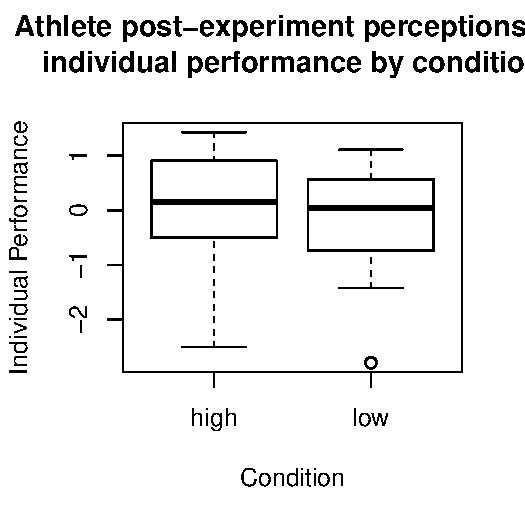
\includegraphics[width=\maxwidth]{figure/indComponentPerformancePostBoxPlot-1} 

}

\end{figure}


\end{knitrout}


\begin{knitrout}
\definecolor{shadecolor}{rgb}{0.969, 0.969, 0.969}\color{fgcolor}\begin{kframe}
\begin{alltt}
\hlstd{groupPerfExpPostBoxPlot} \hlkwb{<-} \hlkwd{boxplot}\hlstd{(groupPerformance_3} \hlopt{~} \hlstd{condition,}
                                        \hlkwc{varwidth} \hlstd{=} \hlnum{TRUE}\hlstd{,}
                                        \hlkwc{width} \hlstd{=} \hlkwd{c}\hlstd{(}\hlnum{.5}\hlstd{,}\hlnum{.5}\hlstd{),}
                                        \hlkwc{notch} \hlstd{= F,}
                                        \hlkwc{main} \hlstd{=} \hlstr{"Athlete post-experiment perceptions of \textbackslash{}n group performance relative to expectations \textbackslash{}n by condition"}\hlstd{,}
                                        \hlkwc{xlab} \hlstd{=} \hlstr{"Condition"}\hlstd{,}
                                        \hlkwc{ylab} \hlstd{=} \hlstr{"Group Performance vs. Expectations"}\hlstd{,}
                                        \hlkwc{data} \hlstd{= twc)}
\end{alltt}
\end{kframe}\begin{figure}

{\centering 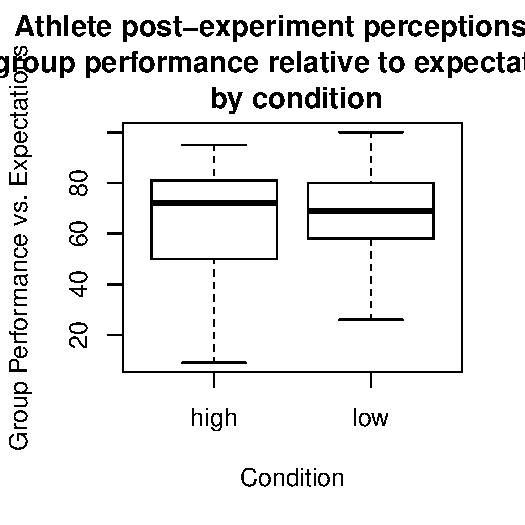
\includegraphics[width=\maxwidth]{figure/groupPerfExpPostBoxPlot-1} 

}

\end{figure}


\end{knitrout}

\begin{knitrout}
\definecolor{shadecolor}{rgb}{0.969, 0.969, 0.969}\color{fgcolor}\begin{kframe}
\begin{alltt}
\hlstd{indPerfExpPostBoxPlot} \hlkwb{<-} \hlkwd{boxplot}\hlstd{(indPerformance_3} \hlopt{~} \hlstd{condition,}
                                        \hlkwc{varwidth} \hlstd{=} \hlnum{TRUE}\hlstd{,}
                                        \hlkwc{width} \hlstd{=} \hlkwd{c}\hlstd{(}\hlnum{.5}\hlstd{,}\hlnum{.5}\hlstd{),}
                                        \hlkwc{notch} \hlstd{= F,}
                                        \hlkwc{main} \hlstd{=} \hlstr{"Athlete post-experiment perceptions of \textbackslash{}n individual performance relative to expectations \textbackslash{}n by condition"}\hlstd{,}
                                        \hlkwc{xlab} \hlstd{=} \hlstr{"Condition"}\hlstd{,}
                                        \hlkwc{ylab} \hlstd{=} \hlstr{"Individual Performance vs. Expectations"}\hlstd{,}
                                        \hlkwc{data} \hlstd{= twc)}
\end{alltt}
\end{kframe}\begin{figure}

{\centering 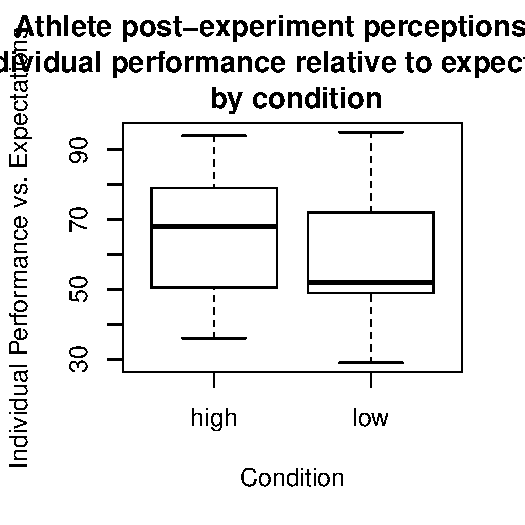
\includegraphics[width=\maxwidth]{figure/indPerfExpPostBoxPlot-1} 

}

\end{figure}

\begin{kframe}\begin{alltt}
\hlcom{# t.test(high$indPerformance_3, low$indPerformance_3)}
\end{alltt}
\end{kframe}
\end{knitrout}


As Table ~\ref{tab:performanceConditionPost} shows, there were no observable significant differences between conditions in athlete perceptions of joint action success, individual component performance, group performance relative to prior expectations, or individual performance relative to prior expectations (see also box plots comparing these factors by condition, Figures ~\ref{fig:groupJointActionSuccessPostBoxPlot}\nobreakdash~\ref{fig:indPerfExpPostBoxPlot}).These results hold when controlling for an athlete's confidence in individual and group performance reported at time 2 prior to the experiment (see APPENDIX for detailed results).













% latex table generated in R 3.3.0 by xtable 1.8-2 package
% Mon Oct 16 10:48:05 2017
\begin{table}[ht]
\centering
\begin{tabular}{rllll}
  \hline
 & high & low & p & test \\ 
  \hline
n &    29 &    29 &  &  \\ 
  GroupClickPost (mean (sd)) & -0.05 (1.07) &  0.05 (0.78) &  0.697 &  \\ 
  GroupBondingPost (mean (sd)) & -0.18 (0.92) & -0.06 (0.79) &  0.616 &  \\ 
  TeamBondingPost (mean (sd)) & -0.12 (0.95) &  0.08 (0.71) &  0.384 &  \\ 
   \hline
\end{tabular}
\caption{Athlete perceptions of click and bonding 
 post-experiment} 
\label{tab:clickBondConditionPost}
\end{table}

%%
%%Table of all factors of interest by condition:
% Performance: individual & group
% group click
% group bonding
% other?
%
\begin{knitrout}
\definecolor{shadecolor}{rgb}{0.969, 0.969, 0.969}\color{fgcolor}\begin{kframe}


{\ttfamily\noindent\color{warningcolor}{\#\# Warning in min(x, na.rm = TRUE): no non-missing arguments to min; returning Inf}}

{\ttfamily\noindent\color{warningcolor}{\#\# Warning in min(x, na.rm = TRUE): no non-missing arguments to min; returning Inf}}

{\ttfamily\noindent\color{warningcolor}{\#\# Warning in min(x, na.rm = TRUE): no non-missing arguments to min; returning Inf}}

{\ttfamily\noindent\color{warningcolor}{\#\# Warning in min(x, na.rm = TRUE): no non-missing arguments to min; returning Inf}}

{\ttfamily\noindent\color{warningcolor}{\#\# Warning in min(x, na.rm = TRUE): no non-missing arguments to min; returning Inf}}

{\ttfamily\noindent\color{warningcolor}{\#\# Warning in min(x, na.rm = TRUE): no non-missing arguments to min; returning Inf}}

{\ttfamily\noindent\color{warningcolor}{\#\# Warning in min(x, na.rm = TRUE): no non-missing arguments to min; returning Inf}}

{\ttfamily\noindent\color{warningcolor}{\#\# Warning in max(x, na.rm = TRUE): no non-missing arguments to max; returning -Inf}}

{\ttfamily\noindent\color{warningcolor}{\#\# Warning in max(x, na.rm = TRUE): no non-missing arguments to max; returning -Inf}}

{\ttfamily\noindent\color{warningcolor}{\#\# Warning in max(x, na.rm = TRUE): no non-missing arguments to max; returning -Inf}}

{\ttfamily\noindent\color{warningcolor}{\#\# Warning in max(x, na.rm = TRUE): no non-missing arguments to max; returning -Inf}}

{\ttfamily\noindent\color{warningcolor}{\#\# Warning in max(x, na.rm = TRUE): no non-missing arguments to max; returning -Inf}}

{\ttfamily\noindent\color{warningcolor}{\#\# Warning in max(x, na.rm = TRUE): no non-missing arguments to max; returning -Inf}}

{\ttfamily\noindent\color{warningcolor}{\#\# Warning in max(x, na.rm = TRUE): no non-missing arguments to max; returning -Inf}}

{\ttfamily\noindent\color{warningcolor}{\#\# Warning in min(x, na.rm = TRUE): no non-missing arguments to min; returning Inf}}

{\ttfamily\noindent\color{warningcolor}{\#\# Warning in min(x, na.rm = TRUE): no non-missing arguments to min; returning Inf}}

{\ttfamily\noindent\color{warningcolor}{\#\# Warning in min(x, na.rm = TRUE): no non-missing arguments to min; returning Inf}}

{\ttfamily\noindent\color{warningcolor}{\#\# Warning in min(x, na.rm = TRUE): no non-missing arguments to min; returning Inf}}

{\ttfamily\noindent\color{warningcolor}{\#\# Warning in max(x, na.rm = TRUE): no non-missing arguments to max; returning -Inf}}

{\ttfamily\noindent\color{warningcolor}{\#\# Warning in max(x, na.rm = TRUE): no non-missing arguments to max; returning -Inf}}

{\ttfamily\noindent\color{warningcolor}{\#\# Warning in max(x, na.rm = TRUE): no non-missing arguments to max; returning -Inf}}

{\ttfamily\noindent\color{warningcolor}{\#\# Warning in max(x, na.rm = TRUE): no non-missing arguments to max; returning -Inf}}

{\ttfamily\noindent\color{warningcolor}{\#\# Warning in StdDiff(variable = var, group = strataVar): Variable has only NA's in at least one stratum. na.rm turned off.}}

{\ttfamily\noindent\color{warningcolor}{\#\# Warning in StdDiff(variable = var, group = strataVar): Variable has only NA's in at least one stratum. na.rm turned off.}}

{\ttfamily\noindent\color{warningcolor}{\#\# Warning in StdDiff(variable = var, group = strataVar): Variable has only NA's in at least one stratum. na.rm turned off.}}

{\ttfamily\noindent\color{warningcolor}{\#\# Warning in StdDiff(variable = var, group = strataVar): Variable has only NA's in at least one stratum. na.rm turned off.}}

{\ttfamily\noindent\color{warningcolor}{\#\# Warning in StdDiff(variable = var, group = strataVar): Variable has only NA's in at least one stratum. na.rm turned off.}}

{\ttfamily\noindent\color{warningcolor}{\#\# Warning in StdDiff(variable = var, group = strataVar): Variable has only NA's in at least one stratum. na.rm turned off.}}

{\ttfamily\noindent\color{warningcolor}{\#\# Warning in StdDiff(variable = var, group = strataVar): Variable has only NA's in at least one stratum. na.rm turned off.}}

{\ttfamily\noindent\color{warningcolor}{\#\# Warning in StdDiff(variable = var, group = strataVar): Variable has only NA's in at least one stratum. na.rm turned off.}}

{\ttfamily\noindent\color{warningcolor}{\#\# Warning in min(x, na.rm = TRUE): no non-missing arguments to min; returning Inf}}

{\ttfamily\noindent\color{warningcolor}{\#\# Warning in min(x, na.rm = TRUE): no non-missing arguments to min; returning Inf}}

{\ttfamily\noindent\color{warningcolor}{\#\# Warning in min(x, na.rm = TRUE): no non-missing arguments to min; returning Inf}}

{\ttfamily\noindent\color{warningcolor}{\#\# Warning in min(x, na.rm = TRUE): no non-missing arguments to min; returning Inf}}

{\ttfamily\noindent\color{warningcolor}{\#\# Warning in min(x, na.rm = TRUE): no non-missing arguments to min; returning Inf}}

{\ttfamily\noindent\color{warningcolor}{\#\# Warning in min(x, na.rm = TRUE): no non-missing arguments to min; returning Inf}}

{\ttfamily\noindent\color{warningcolor}{\#\# Warning in min(x, na.rm = TRUE): no non-missing arguments to min; returning Inf}}

{\ttfamily\noindent\color{warningcolor}{\#\# Warning in max(x, na.rm = TRUE): no non-missing arguments to max; returning -Inf}}

{\ttfamily\noindent\color{warningcolor}{\#\# Warning in max(x, na.rm = TRUE): no non-missing arguments to max; returning -Inf}}

{\ttfamily\noindent\color{warningcolor}{\#\# Warning in max(x, na.rm = TRUE): no non-missing arguments to max; returning -Inf}}

{\ttfamily\noindent\color{warningcolor}{\#\# Warning in max(x, na.rm = TRUE): no non-missing arguments to max; returning -Inf}}

{\ttfamily\noindent\color{warningcolor}{\#\# Warning in max(x, na.rm = TRUE): no non-missing arguments to max; returning -Inf}}

{\ttfamily\noindent\color{warningcolor}{\#\# Warning in max(x, na.rm = TRUE): no non-missing arguments to max; returning -Inf}}

{\ttfamily\noindent\color{warningcolor}{\#\# Warning in max(x, na.rm = TRUE): no non-missing arguments to max; returning -Inf}}

{\ttfamily\noindent\color{warningcolor}{\#\# Warning in min(x, na.rm = TRUE): no non-missing arguments to min; returning Inf}}

{\ttfamily\noindent\color{warningcolor}{\#\# Warning in min(x, na.rm = TRUE): no non-missing arguments to min; returning Inf}}

{\ttfamily\noindent\color{warningcolor}{\#\# Warning in min(x, na.rm = TRUE): no non-missing arguments to min; returning Inf}}

{\ttfamily\noindent\color{warningcolor}{\#\# Warning in min(x, na.rm = TRUE): no non-missing arguments to min; returning Inf}}

{\ttfamily\noindent\color{warningcolor}{\#\# Warning in max(x, na.rm = TRUE): no non-missing arguments to max; returning -Inf}}

{\ttfamily\noindent\color{warningcolor}{\#\# Warning in max(x, na.rm = TRUE): no non-missing arguments to max; returning -Inf}}

{\ttfamily\noindent\color{warningcolor}{\#\# Warning in max(x, na.rm = TRUE): no non-missing arguments to max; returning -Inf}}

{\ttfamily\noindent\color{warningcolor}{\#\# Warning in max(x, na.rm = TRUE): no non-missing arguments to max; returning -Inf}}

{\ttfamily\noindent\color{warningcolor}{\#\# Warning in StdDiff(variable = var, group = strataVar): Variable has only NA's in at least one stratum. na.rm turned off.}}

{\ttfamily\noindent\color{warningcolor}{\#\# Warning in StdDiff(variable = var, group = strataVar): Variable has only NA's in at least one stratum. na.rm turned off.}}

{\ttfamily\noindent\color{warningcolor}{\#\# Warning in StdDiff(variable = var, group = strataVar): Variable has only NA's in at least one stratum. na.rm turned off.}}

{\ttfamily\noindent\color{warningcolor}{\#\# Warning in StdDiff(variable = var, group = strataVar): Variable has only NA's in at least one stratum. na.rm turned off.}}

{\ttfamily\noindent\color{warningcolor}{\#\# Warning in StdDiff(variable = var, group = strataVar): Variable has only NA's in at least one stratum. na.rm turned off.}}

{\ttfamily\noindent\color{warningcolor}{\#\# Warning in StdDiff(variable = var, group = strataVar): Variable has only NA's in at least one stratum. na.rm turned off.}}

{\ttfamily\noindent\color{warningcolor}{\#\# Warning in StdDiff(variable = var, group = strataVar): Variable has only NA's in at least one stratum. na.rm turned off.}}

{\ttfamily\noindent\color{warningcolor}{\#\# Warning in StdDiff(variable = var, group = strataVar): Variable has only NA's in at least one stratum. na.rm turned off.}}\end{kframe}
\end{knitrout}


% latex table generated in R 3.3.0 by xtable 1.8-2 package
% Wed Oct 11 10:01:35 2017
\begin{table}[ht]
\centering
\begin{tabular}{rlllll}
  \hline
 & Baseline & Pre & Post & p & test \\ 
  \hline
n &    29 &    29 &    29 &  &  \\ 
  JointActionSuccess (mean (sd)) &   NaN (NA) &  0.25 (1.00) & -0.40 (1.22) &  0.033 &  \\ 
  IndividualComponentPerformance (mean (sd)) &  0.01 (1.11) &  0.11 (1.06) & -0.02 (1.06) &  0.886 &  \\ 
  GroupPerformanceVsExpectations (mean (sd)) &   NaN (NA) &   NaN (NA) & 66.50 (20.64) &  NA &  \\ 
  IndividualPerformanceExpectations (mean (sd)) &   NaN (NA) &   NaN (NA) & 64.79 (16.83) &  NA &  \\ 
  GroupClick (mean (sd)) &   NaN (NA) &  0.17 (0.82) & -0.28 (1.15) &  0.097 &  \\ 
  GroupBonding (mean (sd)) &   NaN (NA) & -0.01 (0.84) & -0.18 (0.92) &  0.475 &  \\ 
  GroupClickPost (mean (sd)) &   NaN (NA) &   NaN (NA) & -0.05 (1.07) &  NA &  \\ 
  TeamBondingFactor (mean (sd)) & -0.13 (1.04) &   NaN (NA) & -0.12 (0.95) &  0.964 &  \\ 
  Arousal (mean (sd)) &   NaN (NA) & -0.14 (1.00) &  0.12 (1.03) &  0.340 &  \\ 
   \hline
\end{tabular}
\caption{Variables of interest 
 high difficulty condition} 
\label{tab:factorsTimeHigh}
\end{table}

% latex table generated in R 3.5.0 by xtable 1.8-2 package
% Mon Aug 27 19:27:29 2018
\begin{table}[ht]
\centering
\begin{tabular}{rlll}
  \hline
 & Baseline & Pre & Post \\ 
  \hline
n &    29 &    29 &    29 \\ 
  JointActionSuccess (mean (sd)) &   NaN (NA) &  0.30 (0.71) & -0.16 (0.74) \\ 
  IndividualComponentPerformance (mean (sd)) & -0.10 (0.84) &  0.09 (0.79) & -0.10 (0.90) \\ 
  GroupPerformVsExpected (mean (sd)) &   NaN (NA) &   NaN (NA) & 63.55 (20.13) \\ 
  IndividualPerformanceExpectations (mean (sd)) &   NaN (NA) &   NaN (NA) & 58.31 (17.71) \\ 
  GroupClick (mean (sd)) &   NaN (NA) &  0.21 (0.89) & -0.11 (0.77) \\ 
  GroupBonding (mean (sd)) &   NaN (NA) &  0.24 (0.78) & -0.06 (0.79) \\ 
  GroupClickPost (mean (sd)) &   NaN (NA) &   NaN (NA) &  0.05 (0.78) \\ 
  TeamBondingFactor (mean (sd)) &  0.16 (0.80) &   NaN (NA) &  0.08 (0.71) \\ 
  Arousal (mean (sd)) &   NaN (NA) & -0.32 (0.88) &  0.34 (0.79) \\ 
   \hline
\end{tabular}
\caption{Variables of interest 
 low difficulty condition} 
\label{tab:factorsTimeLow}
\end{table}






There were also no observable differences in group click, group bonding, or bonding to team following the experiment (see Tables ~\ref{tab:clickBondConditionPost}\nobreakdash~\ref{tab:factorsTimeLow}).  These results suggest that there was no observable variaiton in athlete self-report according to condition.  Given these results, the entire experiment sample was collapsed into one group and study predictions were tested in this group as a whole.


\begin{knitrout}
\definecolor{shadecolor}{rgb}{0.969, 0.969, 0.969}\color{fgcolor}\begin{kframe}


{\ttfamily\noindent\color{warningcolor}{\#\# Warning in min(x, na.rm = TRUE): no non-missing arguments to min; returning Inf}}

{\ttfamily\noindent\color{warningcolor}{\#\# Warning in min(x, na.rm = TRUE): no non-missing arguments to min; returning Inf}}

{\ttfamily\noindent\color{warningcolor}{\#\# Warning in min(x, na.rm = TRUE): no non-missing arguments to min; returning Inf}}

{\ttfamily\noindent\color{warningcolor}{\#\# Warning in min(x, na.rm = TRUE): no non-missing arguments to min; returning Inf}}

{\ttfamily\noindent\color{warningcolor}{\#\# Warning in min(x, na.rm = TRUE): no non-missing arguments to min; returning Inf}}

{\ttfamily\noindent\color{warningcolor}{\#\# Warning in min(x, na.rm = TRUE): no non-missing arguments to min; returning Inf}}

{\ttfamily\noindent\color{warningcolor}{\#\# Warning in min(x, na.rm = TRUE): no non-missing arguments to min; returning Inf}}

{\ttfamily\noindent\color{warningcolor}{\#\# Warning in max(x, na.rm = TRUE): no non-missing arguments to max; returning -Inf}}

{\ttfamily\noindent\color{warningcolor}{\#\# Warning in max(x, na.rm = TRUE): no non-missing arguments to max; returning -Inf}}

{\ttfamily\noindent\color{warningcolor}{\#\# Warning in max(x, na.rm = TRUE): no non-missing arguments to max; returning -Inf}}

{\ttfamily\noindent\color{warningcolor}{\#\# Warning in max(x, na.rm = TRUE): no non-missing arguments to max; returning -Inf}}

{\ttfamily\noindent\color{warningcolor}{\#\# Warning in max(x, na.rm = TRUE): no non-missing arguments to max; returning -Inf}}

{\ttfamily\noindent\color{warningcolor}{\#\# Warning in max(x, na.rm = TRUE): no non-missing arguments to max; returning -Inf}}

{\ttfamily\noindent\color{warningcolor}{\#\# Warning in max(x, na.rm = TRUE): no non-missing arguments to max; returning -Inf}}

{\ttfamily\noindent\color{warningcolor}{\#\# Warning in min(x, na.rm = TRUE): no non-missing arguments to min; returning Inf}}

{\ttfamily\noindent\color{warningcolor}{\#\# Warning in min(x, na.rm = TRUE): no non-missing arguments to min; returning Inf}}

{\ttfamily\noindent\color{warningcolor}{\#\# Warning in min(x, na.rm = TRUE): no non-missing arguments to min; returning Inf}}

{\ttfamily\noindent\color{warningcolor}{\#\# Warning in min(x, na.rm = TRUE): no non-missing arguments to min; returning Inf}}

{\ttfamily\noindent\color{warningcolor}{\#\# Warning in max(x, na.rm = TRUE): no non-missing arguments to max; returning -Inf}}

{\ttfamily\noindent\color{warningcolor}{\#\# Warning in max(x, na.rm = TRUE): no non-missing arguments to max; returning -Inf}}

{\ttfamily\noindent\color{warningcolor}{\#\# Warning in max(x, na.rm = TRUE): no non-missing arguments to max; returning -Inf}}

{\ttfamily\noindent\color{warningcolor}{\#\# Warning in max(x, na.rm = TRUE): no non-missing arguments to max; returning -Inf}}

{\ttfamily\noindent\color{warningcolor}{\#\# Warning in StdDiff(variable = var, group = strataVar): Variable has only NA's in at least one stratum. na.rm turned off.}}

{\ttfamily\noindent\color{warningcolor}{\#\# Warning in StdDiff(variable = var, group = strataVar): Variable has only NA's in at least one stratum. na.rm turned off.}}

{\ttfamily\noindent\color{warningcolor}{\#\# Warning in StdDiff(variable = var, group = strataVar): Variable has only NA's in at least one stratum. na.rm turned off.}}

{\ttfamily\noindent\color{warningcolor}{\#\# Warning in StdDiff(variable = var, group = strataVar): Variable has only NA's in at least one stratum. na.rm turned off.}}

{\ttfamily\noindent\color{warningcolor}{\#\# Warning in StdDiff(variable = var, group = strataVar): Variable has only NA's in at least one stratum. na.rm turned off.}}

{\ttfamily\noindent\color{warningcolor}{\#\# Warning in StdDiff(variable = var, group = strataVar): Variable has only NA's in at least one stratum. na.rm turned off.}}

{\ttfamily\noindent\color{warningcolor}{\#\# Warning in StdDiff(variable = var, group = strataVar): Variable has only NA's in at least one stratum. na.rm turned off.}}

{\ttfamily\noindent\color{warningcolor}{\#\# Warning in StdDiff(variable = var, group = strataVar): Variable has only NA's in at least one stratum. na.rm turned off.}}\end{kframe}
\end{knitrout}

% latex table generated in R 3.5.0 by xtable 1.8-2 package
% Mon Aug 27 19:27:29 2018
\begin{table}[ht]
\centering
\begin{tabular}{rlll}
  \hline
 & Baseline & Pre & Post \\ 
  \hline
n &    58 &    58 &    58 \\ 
  JointActionSuccess (mean (sd)) &   NaN (NA) &  0.27 (0.86) & -0.28 (1.01) \\ 
  IndividualComponentPerformance (mean (sd)) & -0.05 (0.98) &  0.10 (0.93) & -0.06 (0.97) \\ 
  GroupPerformVsExpected (mean (sd)) &   NaN (NA) &   NaN (NA) & 63.37 (21.23) \\ 
  IndividualPerformanceExpectations (mean (sd)) &   NaN (NA) &   NaN (NA) & 61.49 (17.44) \\ 
  GroupClick (mean (sd)) &   NaN (NA) &  0.19 (0.85) & -0.19 (0.97) \\ 
  GroupBonding (mean (sd)) &   NaN (NA) &  0.12 (0.81) & -0.12 (0.85) \\ 
  GroupClickPost (mean (sd)) &   NaN (NA) &   NaN (NA) & -0.00 (0.93) \\ 
  TeamBondingFactor (mean (sd)) &  0.02 (0.93) &   NaN (NA) & -0.02 (0.84) \\ 
  Arousal (mean (sd)) &   NaN (NA) & -0.23 (0.94) &  0.23 (0.92) \\ 
   \hline
\end{tabular}
\caption{Variables of interest over time 
 for entire sample} 
\label{tab:factorsTime}
\end{table}


Table ~\ref{tab:factorsTime} shows that factors relating to group Joint Action Success, Group Click reduced between pre- and post-Experiment measurements.  Group Bonding also appeared to reduce, but this change was not significant.  Athlete reports of arousal significantly increased following the experiment, as would be expected due to the moderate to high levels of physiological exertion associated with the training drill.  Athlete perceptions of components of individual performance and bonding to the team as a whole did not vary significantly acrross time points.


\subsubsection{post-Experiment Survey Data}

Study predictions were first tested using the post-Experiment survey data.

\myparagraph{Prediction 1.a: higher perceptions of Joint Action Success will correlate with higher feelings of team click with the training group}

\begin{knitrout}
\definecolor{shadecolor}{rgb}{0.969, 0.969, 0.969}\color{fgcolor}\begin{kframe}
\begin{alltt}
\hlstd{apatheme}\hlkwb{=}\hlkwd{theme_bw}\hlstd{()}\hlopt{+}
  \hlkwd{theme}\hlstd{(}\hlkwc{panel.grid.major}\hlstd{=}\hlkwd{element_blank}\hlstd{(),}
        \hlkwc{panel.grid.minor}\hlstd{=}\hlkwd{element_blank}\hlstd{(),}
        \hlkwc{panel.border}\hlstd{=}\hlkwd{element_blank}\hlstd{(),}
        \hlkwc{axis.line}\hlstd{=}\hlkwd{element_line}\hlstd{(),}
        \hlkwc{text}\hlstd{=}\hlkwd{element_text}\hlstd{(}\hlkwc{family}\hlstd{=}\hlstr{'Times'}\hlstd{))}

\hlstd{jASClickScatter} \hlkwb{<-} \hlkwd{ggplot}\hlstd{(twc,} \hlkwd{aes}\hlstd{(}\hlkwc{x}\hlstd{=jointActionSuccessPost,} \hlkwc{y}\hlstd{=groupClickPostFactor,}
                            \hlkwc{color}\hlstd{=condition))} \hlopt{+} \hlkwd{geom_point}\hlstd{(}\hlkwc{shape} \hlstd{=} \hlnum{1}\hlstd{)} \hlopt{+}
                            \hlkwd{geom_smooth}\hlstd{(}\hlkwc{method}\hlstd{=lm,} \hlkwc{se}\hlstd{=}\hlnum{FALSE}\hlstd{)}   \hlcom{# Don't add shaded confidence region}
\hlstd{jASClickScatter} \hlopt{+}
            \hlkwd{ggtitle}\hlstd{(}\hlstr{"Joint Action Success predicts Group Click"}\hlstd{)} \hlopt{+}
            \hlkwd{theme}\hlstd{(}\hlkwc{plot.title} \hlstd{=} \hlkwd{element_text}\hlstd{(}\hlkwc{hjust}\hlstd{=}\hlnum{0}\hlstd{,} \hlkwc{size}\hlstd{=}\hlnum{12}\hlstd{))} \hlopt{+}
            \hlkwd{xlab}\hlstd{(}\hlstr{"Joing Action Success"}\hlstd{)} \hlopt{+}
            \hlkwd{ylab}\hlstd{(}\hlstr{"Group Click"}\hlstd{)} \hlopt{+}
            \hlstd{apatheme}
\end{alltt}


{\ttfamily\noindent\color{warningcolor}{\#\# Warning: Removed 1 rows containing non-finite values (stat\_smooth).}}

{\ttfamily\noindent\color{warningcolor}{\#\# Warning: Removed 1 rows containing missing values (geom\_point).}}\end{kframe}\begin{figure}

{\centering 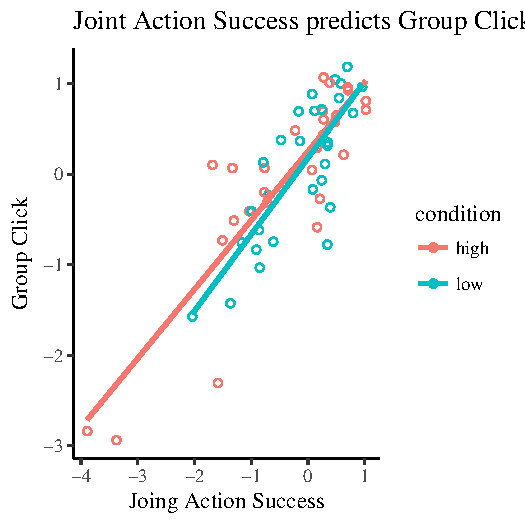
\includegraphics[width=\maxwidth]{figure/jASClickScatter-1} 

}

\end{figure}


\end{knitrout}

Figure ~\ref{fig:jASClickScatter} shows a strong positive correlation between perceived joint action success and feelings of ``team click'' with the training group post-Experiment.

MODEL:


\myparagraph{Prediction 1.b: More positive violations of expectations around team performance will correlate with higer feelings of team click with the training group}

\begin{knitrout}
\definecolor{shadecolor}{rgb}{0.969, 0.969, 0.969}\color{fgcolor}\begin{kframe}
\begin{alltt}
\hlstd{groupPerfExpClickScatter} \hlkwb{<-} \hlkwd{ggplot}\hlstd{(twc,} \hlkwd{aes}\hlstd{(}\hlkwc{x}\hlstd{=groupPerformance_3,} \hlkwc{y}\hlstd{=groupClickPostFactor,}
                            \hlkwc{color}\hlstd{=condition))} \hlopt{+} \hlkwd{geom_point}\hlstd{(}\hlkwc{shape} \hlstd{=} \hlnum{1}\hlstd{)} \hlopt{+}
                            \hlkwd{geom_smooth}\hlstd{(}\hlkwc{method}\hlstd{=lm,} \hlkwc{se}\hlstd{=}\hlnum{FALSE}\hlstd{)}   \hlcom{# Don't add shaded confidence region}
\hlstd{groupPerfExpClickScatter} \hlopt{+}
            \hlkwd{ggtitle}\hlstd{(}\hlstr{"Positive violation of Team Performance Expectations \textbackslash{}n predicts Group Click"}\hlstd{)} \hlopt{+}
            \hlkwd{theme}\hlstd{(}\hlkwc{plot.title} \hlstd{=} \hlkwd{element_text}\hlstd{(}\hlkwc{size}\hlstd{=}\hlnum{12}\hlstd{))} \hlopt{+}
            \hlkwd{xlab}\hlstd{(}\hlstr{"Team Performance vs Expectations"}\hlstd{)} \hlopt{+}
            \hlkwd{ylab}\hlstd{(}\hlstr{"Group Click"}\hlstd{)} \hlopt{+}
            \hlstd{apatheme}
\end{alltt}


{\ttfamily\noindent\color{warningcolor}{\#\# Warning: Removed 1 rows containing non-finite values (stat\_smooth).}}

{\ttfamily\noindent\color{warningcolor}{\#\# Warning: Removed 1 rows containing missing values (geom\_point).}}\end{kframe}\begin{figure}

{\centering 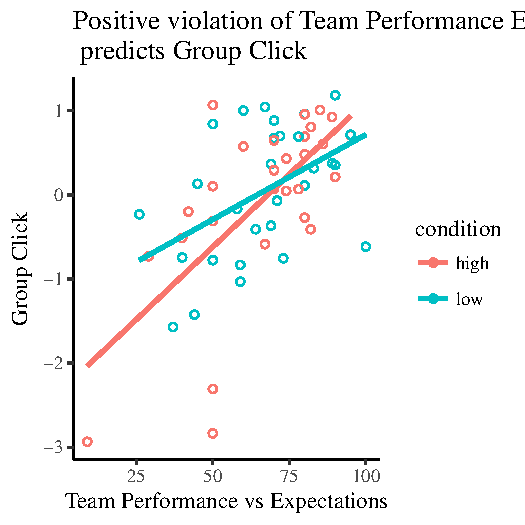
\includegraphics[width=\maxwidth]{figure/teamPerfExpClickScatter-1} 

}

\end{figure}


\end{knitrout}

Figure ~\ref{fig:teamPerfExpClickScatter} shows a strong positive correlation between violations of expectations around team performance and feelings of ``team click'' with the training group post-Experiment.

MODEL:



\myparagraph{Prediction 1.c: More positive violations of expectations around team performance will correlate with higer feelings of team click with the training group}

\begin{knitrout}
\definecolor{shadecolor}{rgb}{0.969, 0.969, 0.969}\color{fgcolor}\begin{kframe}
\begin{alltt}
\hlstd{twc}\hlopt{$}\hlstd{groupPerformance_3} \hlkwb{<-} \hlkwd{scale}\hlstd{(twc}\hlopt{$}\hlstd{groupPerformance_3)}
\hlstd{jASPerfExpCLick} \hlkwb{<-} \hlkwd{lm}\hlstd{(groupClickPostFactor} \hlopt{~} \hlstd{jointActionSuccessPost}\hlopt{*}\hlstd{groupPerformance_3,} \hlkwc{data} \hlstd{= twc)}
\hlcom{## use vcov() to get parameter variances and covariances for Kris’s interaction utility}
\hlkwd{vcov}\hlstd{(jASPerfExpCLick)}
\hlcom{## degrees of freedom for the model from the summary of the regression model}
\hlkwd{summary}\hlstd{(jASPerfExpCLick)}
\hlcom{## used the psych package’s describe function to get the mean and standard deviation of groupClick}
\hlstd{psych}\hlopt{::}\hlkwd{describe}\hlstd{(twc}\hlopt{$}\hlstd{groupClickPostFactor)}
\hlkwd{min}\hlstd{(twc}\hlopt{$}\hlstd{jointActionSuccessPost,} \hlkwc{na.rm}\hlstd{=T)}
\hlkwd{max}\hlstd{(twc}\hlopt{$}\hlstd{jointActionSuccessPost,} \hlkwc{na.rm}\hlstd{=T)}
\hlcom{##OUTPUT##}
\hlcom{#Simple Intercepts and Slopes at Conditional Values of Z}
\hlcom{#=======================================================}
\hlcom{#At Z = cv1... (-1SD)}
\hlcom{#  simple intercept = 0.16(0.1267), t=1.2626, p=0.2123}
\hlcom{#  simple slope     = 0.7371(0.0851), t=8.6581, p=0}
\hlcom{#At Z = cv2... (Mean)}
\hlcom{#  simple intercept = 0.2242(0.0737), t=3.0419, p=0.0037}
\hlcom{#  simple slope     = 0.6815(0.0894), t=7.6199, p=0}
\hlcom{#At Z = cv3... (+1SD)}
\hlcom{#  simple intercept = 0.2885(0.0931), t=3.0988, p=0.0031}
\hlcom{#  simple slope     = 0.6259(0.12), t=5.2164, p=0}
\hlstd{jASGroupPerfExpClickScatter} \hlkwb{<-} \hlkwd{ggplot}\hlstd{(twc,} \hlkwd{aes}\hlstd{(}\hlkwc{x}\hlstd{=jointActionSuccessPost,}
                                      \hlkwc{y}\hlstd{=groupClickPostFactor,} \hlkwc{size}\hlstd{=groupPerformance_3))} \hlopt{+} \hlkwd{geom_point}\hlstd{()}
\hlstd{jASGroupPerfExpClickScatter} \hlopt{+}
            \hlkwd{ggtitle}\hlstd{(}\hlstr{"Positive violation of Team Performance Expectations \textbackslash{}n predicts Group Click"}\hlstd{)} \hlopt{+}
            \hlkwd{theme}\hlstd{(}\hlkwc{plot.title} \hlstd{=} \hlkwd{element_text}\hlstd{(}\hlkwc{size}\hlstd{=}\hlnum{12}\hlstd{))} \hlopt{+}
            \hlkwd{xlab}\hlstd{(}\hlstr{"Joint Action Success"}\hlstd{)} \hlopt{+}
            \hlkwd{ylab}\hlstd{(}\hlstr{"Group Click"}\hlstd{)} \hlopt{+}
            \hlkwd{scale_size_continuous}\hlstd{(}\hlkwc{guide} \hlstd{=} \hlnum{FALSE}\hlstd{)}\hlopt{+}
            \hlkwd{geom_abline}\hlstd{(}\hlkwd{aes}\hlstd{(}\hlkwc{intercept}\hlstd{=}\hlnum{0.16}\hlstd{,} \hlkwc{slope}\hlstd{=}\hlnum{0.7371}\hlstd{,} \hlkwc{linetype}\hlstd{=}\hlstr{'-1SD TeamPerformanceExpectation'}\hlstd{))}\hlopt{+}
            \hlkwd{geom_abline}\hlstd{(}\hlkwd{aes}\hlstd{(}\hlkwc{intercept}\hlstd{=}\hlnum{0.2242}\hlstd{,} \hlkwc{slope}\hlstd{=}\hlnum{0.6815}\hlstd{,} \hlkwc{linetype}\hlstd{=}\hlstr{'Mean TeamPerformanceExpectation'}\hlstd{))}\hlopt{+}
            \hlkwd{geom_abline}\hlstd{(}\hlkwd{aes}\hlstd{(}\hlkwc{intercept}\hlstd{=}\hlnum{0.2885}\hlstd{,} \hlkwc{slope}\hlstd{=}\hlnum{0.6259}\hlstd{,} \hlkwc{linetype}\hlstd{=}\hlstr{'+1SDTeamPerformanceExpectation'}\hlstd{))}\hlopt{+}
            \hlkwd{scale_linetype_manual}\hlstd{(}\hlkwc{values}\hlstd{=}\hlkwd{c}\hlstd{(}\hlstr{'dotted'}\hlstd{,}\hlstr{'dashed'}\hlstd{,}\hlstr{'solid'}\hlstd{),}
            \hlkwc{breaks}\hlstd{=}\hlkwd{c}\hlstd{(}\hlstr{'-1SD Gear'}\hlstd{,}\hlstr{'Mean Gear'}\hlstd{,}\hlstr{'+1SD Gear'}\hlstd{),}\hlkwc{name}\hlstd{=}\hlstr{'Simple\textbackslash{}nSlope'}\hlstd{)}\hlopt{+}
            \hlstd{apatheme}
\end{alltt}


{\ttfamily\noindent\color{warningcolor}{\#\# Warning: Removed 1 rows containing missing values (geom\_point).}}\end{kframe}\begin{figure}

{\centering 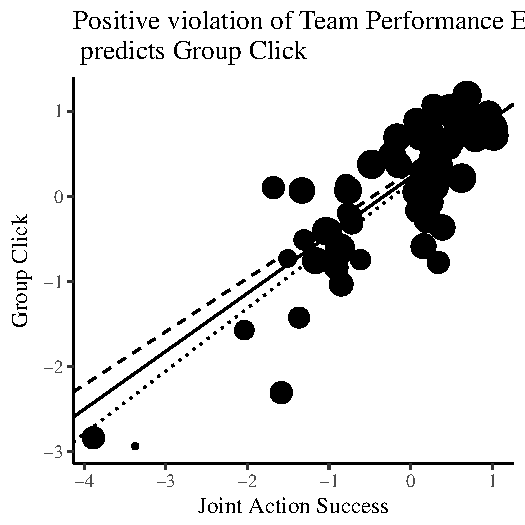
\includegraphics[width=\maxwidth]{figure/jASGroupPerfExpClickScatter-1} 

}

\end{figure}


\end{knitrout}

Figure ~\ref{fig:jASGroupPerfExpClickScatter} displays the relationship between perceptions of Joint Action Success and Group Click, moderated by perceptions of Team Performance expectations.  There does not appear to be a strong moderating effect of team performance expectation violation on the relationship between these two variables.

MODEL:

\myparagraph{Prediction 2.a: Feelings of group click will positively correlate with feelings of social bonding to the group}

\begin{knitrout}
\definecolor{shadecolor}{rgb}{0.969, 0.969, 0.969}\color{fgcolor}\begin{kframe}
\begin{alltt}
\hlstd{groupClickBondScatter} \hlkwb{<-} \hlkwd{ggplot}\hlstd{(twc,} \hlkwd{aes}\hlstd{(}\hlkwc{x}\hlstd{=groupClickPostFactor,} \hlkwc{y}\hlstd{=groupBondingFactorPost,}
                            \hlkwc{color}\hlstd{=condition))} \hlopt{+} \hlkwd{geom_point}\hlstd{(}\hlkwc{shape} \hlstd{=} \hlnum{1}\hlstd{)} \hlopt{+}
                            \hlkwd{geom_smooth}\hlstd{(}\hlkwc{method}\hlstd{=lm,} \hlkwc{se}\hlstd{=}\hlnum{FALSE}\hlstd{)}   \hlcom{# Don't add shaded confidence region}
\hlstd{groupClickBondScatter} \hlopt{+}
            \hlkwd{ggtitle}\hlstd{(}\hlstr{"Perceptions of Group Click \textbackslash{}n predict feelings of Social Bonding to training group"}\hlstd{)} \hlopt{+}
            \hlkwd{theme}\hlstd{(}\hlkwc{plot.title} \hlstd{=} \hlkwd{element_text}\hlstd{(}\hlkwc{size}\hlstd{=}\hlnum{12}\hlstd{))} \hlopt{+}
            \hlkwd{xlab}\hlstd{(}\hlstr{"Group Click"}\hlstd{)} \hlopt{+}
            \hlkwd{ylab}\hlstd{(}\hlstr{"Social Bonding"}\hlstd{)} \hlopt{+}
            \hlstd{apatheme}
\end{alltt}


{\ttfamily\noindent\color{warningcolor}{\#\# Warning: Removed 1 rows containing non-finite values (stat\_smooth).}}

{\ttfamily\noindent\color{warningcolor}{\#\# Warning: Removed 1 rows containing missing values (geom\_point).}}\end{kframe}\begin{figure}

{\centering 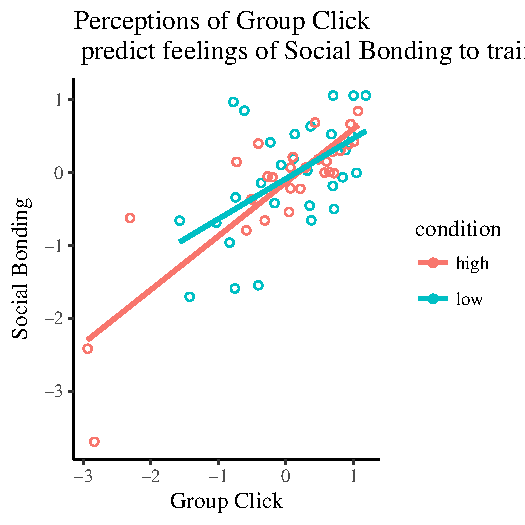
\includegraphics[width=\maxwidth]{figure/groupClickBondScatter-1} 

}

\end{figure}


\end{knitrout}

Figure ~\ref{fig:groupClickBondScatter} shows a clear relationship between Group Click and Social Bonding to the training group following the training group.


MODEL:



\myparagraph{Prediction 3.a: Perceptions of higher Joint Action Success will predict higher levels of Social Bonding to the training group}


\begin{knitrout}
\definecolor{shadecolor}{rgb}{0.969, 0.969, 0.969}\color{fgcolor}\begin{kframe}
\begin{alltt}
\hlstd{jASBondScatter} \hlkwb{<-} \hlkwd{ggplot}\hlstd{(twc,} \hlkwd{aes}\hlstd{(}\hlkwc{x}\hlstd{=jointActionSuccessPost,} \hlkwc{y}\hlstd{=groupBondingFactorPost,}
                            \hlkwc{color}\hlstd{=condition))} \hlopt{+} \hlkwd{geom_point}\hlstd{(}\hlkwc{shape} \hlstd{=} \hlnum{1}\hlstd{)} \hlopt{+}
                            \hlkwd{geom_smooth}\hlstd{(}\hlkwc{method}\hlstd{=lm,} \hlkwc{se}\hlstd{=}\hlnum{FALSE}\hlstd{)}
\hlstd{jASBondScatter} \hlopt{+}
            \hlkwd{ggtitle}\hlstd{(}\hlstr{"Perceptions of Joint Action Success \textbackslash{}n predict feelings of Social Bonding to training group"}\hlstd{)} \hlopt{+}
            \hlkwd{theme}\hlstd{(}\hlkwc{plot.title} \hlstd{=} \hlkwd{element_text}\hlstd{(}\hlkwc{size}\hlstd{=}\hlnum{12}\hlstd{))} \hlopt{+}
            \hlkwd{xlab}\hlstd{(}\hlstr{"Joint Action Success"}\hlstd{)} \hlopt{+}
            \hlkwd{ylab}\hlstd{(}\hlstr{"Social Bonding"}\hlstd{)} \hlopt{+}
            \hlstd{apatheme}
\end{alltt}


{\ttfamily\noindent\color{warningcolor}{\#\# Warning: Removed 1 rows containing non-finite values (stat\_smooth).}}

{\ttfamily\noindent\color{warningcolor}{\#\# Warning: Removed 1 rows containing missing values (geom\_point).}}\end{kframe}\begin{figure}

{\centering 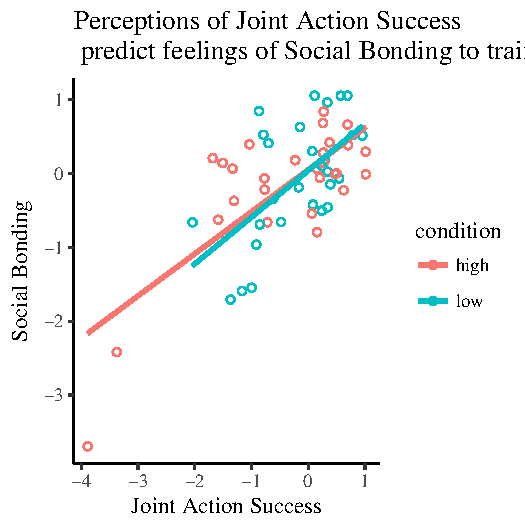
\includegraphics[width=\maxwidth]{figure/jASBondScatter-1} 

}

\end{figure}


\end{knitrout}

Figure ~\ref{fig:jASBondScatter} shows a strong positive relationship between Joint Action Success and Social Bonding to the training group, suggesting that athletes who perceived greater success in components of joint action also felt higher levels of social bonding to their co-actors in the training drill.

MODEL:



\myparagraph{Prediction 3.a: Perceptions of higher Joint Action Success will predict higher levels of Social Bonding to the training group}


\begin{knitrout}
\definecolor{shadecolor}{rgb}{0.969, 0.969, 0.969}\color{fgcolor}\begin{kframe}
\begin{alltt}
\hlstd{teamPerfExpBondScatter} \hlkwb{<-} \hlkwd{ggplot}\hlstd{(twc,} \hlkwd{aes}\hlstd{(}\hlkwc{x}\hlstd{=groupPerformance_3,} \hlkwc{y}\hlstd{=groupBondingFactorPost,}
                            \hlkwc{color}\hlstd{=condition))} \hlopt{+} \hlkwd{geom_point}\hlstd{(}\hlkwc{shape} \hlstd{=} \hlnum{1}\hlstd{)} \hlopt{+}
                            \hlkwd{geom_smooth}\hlstd{(}\hlkwc{method}\hlstd{=lm,} \hlkwc{se}\hlstd{=}\hlnum{FALSE}\hlstd{)}
\hlstd{teamPerfExpBondScatter} \hlopt{+}
            \hlkwd{ggtitle}\hlstd{(}\hlstr{"Perceptions of Team Performance (vs prior expectations) \textbackslash{}n predict feelings of Social Bonding to training group"}\hlstd{)} \hlopt{+}
            \hlkwd{theme}\hlstd{(}\hlkwc{plot.title} \hlstd{=} \hlkwd{element_text}\hlstd{(}\hlkwc{size}\hlstd{=}\hlnum{12}\hlstd{))} \hlopt{+}
            \hlkwd{xlab}\hlstd{(}\hlstr{"Team Performance vs Prior Expectations"}\hlstd{)} \hlopt{+}
            \hlkwd{ylab}\hlstd{(}\hlstr{"Social Bonding"}\hlstd{)} \hlopt{+}
            \hlstd{apatheme}
\end{alltt}


{\ttfamily\noindent\color{warningcolor}{\#\# Warning: Removed 1 rows containing non-finite values (stat\_smooth).}}

{\ttfamily\noindent\color{warningcolor}{\#\# Warning: Removed 1 rows containing missing values (geom\_point).}}\end{kframe}\begin{figure}

{\centering 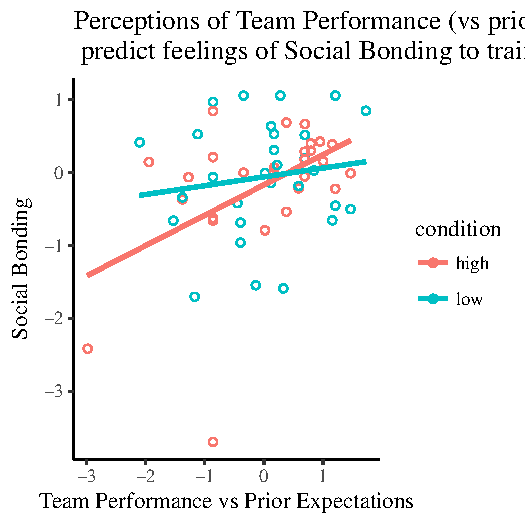
\includegraphics[width=\maxwidth]{figure/teamPerfExpBondScatter-1} 

}

\end{figure}


\end{knitrout}

\begin{knitrout}
\definecolor{shadecolor}{rgb}{0.969, 0.969, 0.969}\color{fgcolor}\begin{kframe}
\begin{alltt}
\hlstd{teamPerfExpBondScatter1} \hlkwb{<-} \hlkwd{ggplot}\hlstd{(twc,} \hlkwd{aes}\hlstd{(}\hlkwc{x}\hlstd{=groupPerformance_3,} \hlkwc{y}\hlstd{=groupBondingFactorPost))} \hlopt{+} \hlkwd{geom_point}\hlstd{(}\hlkwc{shape} \hlstd{=} \hlnum{1}\hlstd{)} \hlopt{+}
                            \hlkwd{geom_smooth}\hlstd{(}\hlkwc{method}\hlstd{=lm,} \hlkwc{se}\hlstd{=}\hlnum{FALSE}\hlstd{)}
\hlstd{teamPerfExpBondScatter1} \hlopt{+}
            \hlkwd{ggtitle}\hlstd{(}\hlstr{"Perceptions of Team Performance (vs prior expectations) \textbackslash{}n predict feelings of Social Bonding to training group"}\hlstd{)} \hlopt{+}
            \hlkwd{theme}\hlstd{(}\hlkwc{plot.title} \hlstd{=} \hlkwd{element_text}\hlstd{(}\hlkwc{size}\hlstd{=}\hlnum{12}\hlstd{))} \hlopt{+}
            \hlkwd{xlab}\hlstd{(}\hlstr{"Team Performance vs Prior Expectations"}\hlstd{)} \hlopt{+}
            \hlkwd{ylab}\hlstd{(}\hlstr{"Social Bonding"}\hlstd{)} \hlopt{+}
            \hlstd{apatheme}
\end{alltt}


{\ttfamily\noindent\color{warningcolor}{\#\# Warning: Removed 1 rows containing non-finite values (stat\_smooth).}}

{\ttfamily\noindent\color{warningcolor}{\#\# Warning: Removed 1 rows containing missing values (geom\_point).}}\end{kframe}\begin{figure}

{\centering 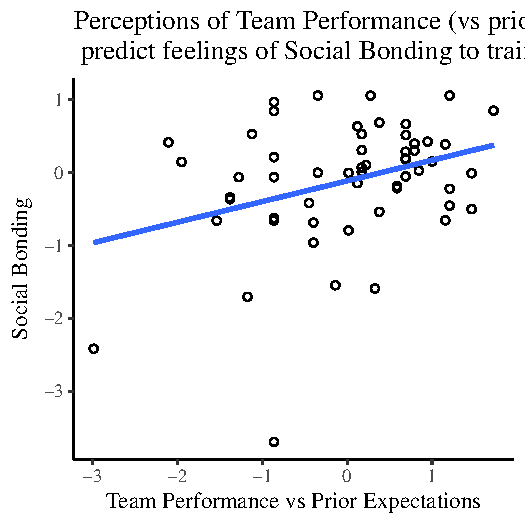
\includegraphics[width=\maxwidth]{figure/teamPerfExpBondScatter1-1} 

}

\end{figure}


\end{knitrout}


Figure ~\ref{fig:teamPerfExpBondScatter1} shows an overall positive correlation between perceptions of Joint Action Success and Social Bonding to the training group.  When this relationship is moderated by condition, as shown in Figure ~\ref{fig:teamPerfExpBondScatter}, it appears that the positive relationship is being driven by results in the high difficulty condition.

MODEL: the interaction between group performance and condition was not significant.
















\begin{knitrout}
\definecolor{shadecolor}{rgb}{0.969, 0.969, 0.969}\color{fgcolor}\begin{kframe}


{\ttfamily\noindent\color{warningcolor}{\#\# Warning: package 'lme4' was built under R version 3.3.2}}

{\ttfamily\noindent\itshape\color{messagecolor}{\#\# Loading required package: Matrix}}

{\ttfamily\noindent\bfseries\color{errorcolor}{\#\# Error: 'data' not found, and some variables missing from formula environment}}

{\ttfamily\noindent\bfseries\color{errorcolor}{\#\# Error: 'data' not found, and some variables missing from formula environment}}

{\ttfamily\noindent\bfseries\color{errorcolor}{\#\# Error in summary(bondingCondTime.lmer): object 'bondingCondTime.lmer' not found}}

{\ttfamily\noindent\bfseries\color{errorcolor}{\#\# Error: 'data' not found, and some variables missing from formula environment}}\end{kframe}
\end{knitrout}




\begin{knitrout}
\definecolor{shadecolor}{rgb}{0.969, 0.969, 0.969}\color{fgcolor}

{\centering 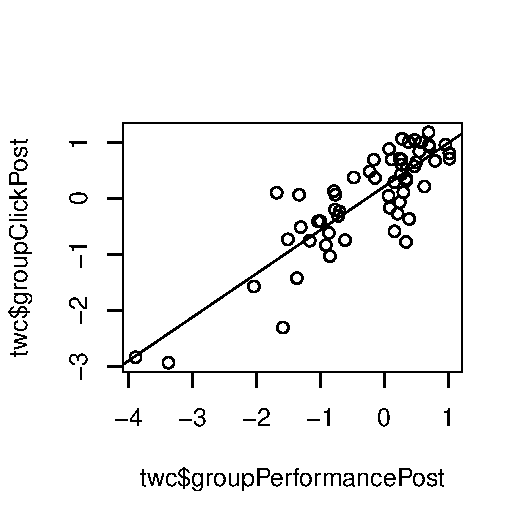
\includegraphics[width=\maxwidth]{figure/predictionsTest-1} 

}




{\centering 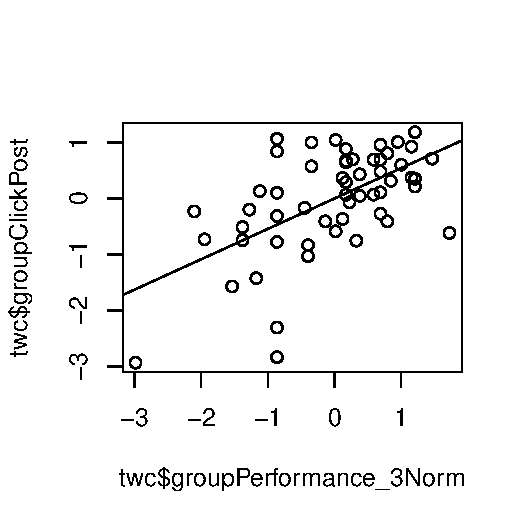
\includegraphics[width=\maxwidth]{figure/predictionsTest-2} 

}




{\centering 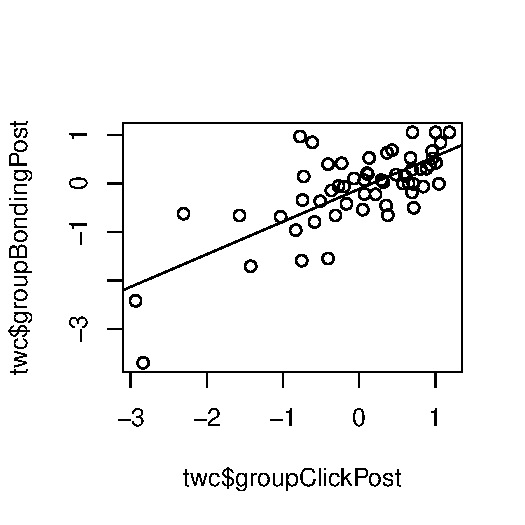
\includegraphics[width=\maxwidth]{figure/predictionsTest-3} 

}




{\centering 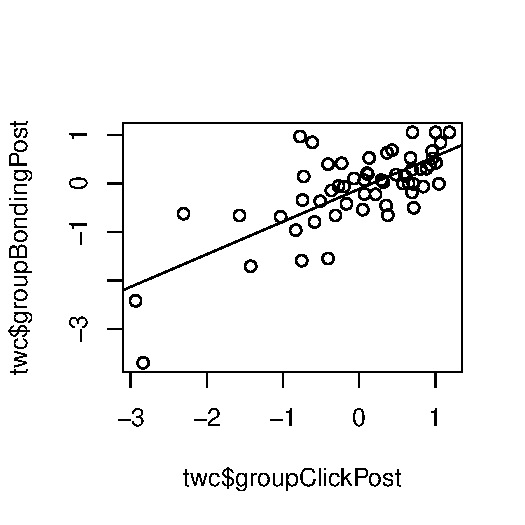
\includegraphics[width=\maxwidth]{figure/predictionsTest-4} 

}



\end{knitrout}


























%\section{Discussion}
%1.Summary of the research:


{\renewcommand*\MakeUppercase[1]{#1}%
\printbibliography[heading=bibintoc,title={\bibtitle}]}



\end{document}
